\documentclass
[
    twoside,                 % The thesis is formatted like a book. That is, odd and even pages are handled differently.
    openright,               % Starts a new chapter on an odd page number (right side).
    cleardoublepage = empty, % Clear pages inserted in order to have new chapters appear on odd pages are formatted with an empty style.
    fontsize = 12 pt,        % The size of the font.
    british,                 % Support for British English.
    captions = tableheading, % Places the correct amount of space when the caption of a table is above the table.
    numbers = noenddot,      % Does not use a period at the end of numbered titles, such as sections or figures.
    footheight = 35 pt,      % Defines the height of the foot. Due to the line, it needs extra height.
%    draft,                   % Only displays boxes of figures. This option is useful if compilation takes a long time.
]
{scrbook}


% This file contains all sorts of commands that are used in order to specify certain options for the document.

\newif\ifprintVersion   % Defines a binary variable that signals whether the document is prepared for physical or digital print.
\newif\ifprofessionalPrint % Defines a binary variable that signals whether the print will be done by a professional printing service that requests extra margin for page cutting and is not bound to paper formats like A4.
\newif\iffancyTheorems  % Defines a binary variable that signals whether theorems are formatted in the classical style or in a new format that better suits the overall flavor of this thesis.
\newif\ifboldNumberSets % Defines a binary variable that signals whether the variables for number sets (like N or R) should be in bold. If not, they are in blackboard bold instead.
\newif\ifbachelorThesis % Defines a binary variable that signals whether this thesis is a bachelor thesis (true) or a master thesis (false).

% Set all variables to their default values.
\printVersionfalse
\professionalPrintfalse
\fancyTheoremstrue
\boldNumberSetstrue
\bachelorThesistrue

%%%%%%%%%%%%%%%%%%%%%%%%
% The following commands define certain strings that provide important information for the document.

% The title of the thesis.
\newcommand*{\printTitle}{}
\newcommand*{\printGermanTitle}{}
\newcommand*{\myTitle}[2]{\renewcommand*{\printTitle}{#1}\renewcommand*{\printGermanTitle}{#2}}
\newcommand*{\printTitleBold}{\textbf{\printTitle}}

% The author’s name.
\newcommand*{\printAuthor}{}
\newcommand*{\myName}[1]{\renewcommand*{\printAuthor}{#1}}

% The name of the author’s program.
\newcommand*{\printProgram}{}
\newcommand*{\myProgram}[1]{\renewcommand*{\printProgram}{#1}}

% The date when the thesis was handed in.
\newcommand*{\printDateReceived}{}
\newcommand*{\dateOfHandingIn}[1]{\renewcommand*{\printDateReceived}{#1}}

% A short description of the topic of the thesis. This string will be used for the PDF metadata.
\newcommand*{\printSubject}{}
\newcommand*{\mySubject}[1]{\renewcommand*{\printSubject}{#1}}

% A short description of the topic of the thesis. This string will be used for the PDF metadata.
\newcommand*{\printKeywords}{}
\newcommand*{\myKeywords}[1]{\renewcommand*{\printKeywords}{#1}}

% The name of the author’s supervisor.
\newcommand*{\printNameOfSupervisor}{}
\newcommand*{\nameOfMySupervisor}[1]{\renewcommand*{\printNameOfSupervisor}{#1}}

% The list with the name of the additional examiners.
\newcommand*{\printAdditionalExaminers}{}
\newcommand*{\additionalExaminers}[1]{\renewcommand*{\printAdditionalExaminers}{#1}}

% Defines the extra length added to each side for the print version.
\newlength{\extraborderlength}
\newcommand*{\extraBorder}[1]{\setlength{\extraborderlength}{#1}}

% Defines the length of the binding correction. (The class ›scrbook‹ has a binding correction but it does not work due to all the other packages that are loaded.)
\newlength{\mybindingcorrection}
\newcommand*{\bindingCorrection}[1]{\setlength{\mybindingcorrection}{#1}} % Contains commands that are used for certain information that is printed.


%%%%%%%%%%%%%%%%%%%%%%%%%%%%%%%%%%%%%%
%% Please adjust your options here. %%
%%%%%%%%%%%%%%%%%%%%%%%%%%%%%%%%%%%%%%

    % This section contains commands with important data for your thesis. Please adjust them in order for the document to be printed correctly.

    % Defines the length of the amount that a printed page will be cut from EACH side (including the inner side). This option only takes effect with \printVersiontrue and \professionalPrinttrue.
    \extraBorder{3 mm}

    % Shifts the inner margin outward by the amount specified. When the book is bound, part of the page will not be seen anymore. This option compensates for this loss. It only takes effect with \printVersiontrue.
    \bindingCorrection{6 mm}

    % Use the following command if this is a master thesis.
%    \bachelorThesisfalse

%    \printVersiontrue      % Use this value if you want to prepare your thesis for physical printing. In this case, links will not be coloured. Without \professionalPrinttrue, the content will be moved outward by the binding correction, increasing the inner margin and decreasing the outer margin.
%    \professionalPrinttrue % Use this value if you want to have extra border for cutting and are not bound to paper formats (like A4). This option will increase the page size by the extra border on every side plus the binding correction once for the width. It only takes effect in combination with \printVersiontrue.
%    \fancyTheoremsfalse  % Use this value if you want to use the classical theorem style, where the text is italic. Further, with this style, the QED symbol is colourless.
%    \boldNumberSetsfalse % Use this value if you want variables for number sets (like N or R) to appear in blackboard bold rather than bold.

    % The title of the thesis. The first argument is for the English name, the second is for the German name.
    \myTitle{Monitoring of Agents for Dynamic Pricing in different (Re-)Commerce Markets}
	{Monitoring von Agenten zur dynamischen Bepreisung in unterschiedlichen (Re-)Commerce Märkten}

    % The author’s name.
    \myName{Nikkel Mollenhauer}

    % The author’s program.
    \myProgram{IT-Systems Engineering}

    % The date when the thesis will be handed in.
    \dateOfHandingIn{30. Juni 2022}

    % The name and affiliation of the author’s supervisor.
    \nameOfMySupervisor{Dr. Michael Perscheid}

    % A list with the names of the additional examiners.
    \additionalExaminers{Dr. Rainer Schlosser\newline Johannes Huegle\newline Alexander Kastius}

    % A short summary of the thesis. This information will be used for the PDF meta data.
    \mySubject{Bachelor thesis concerning the monitoring and subsequent evaluation of Reinforcement Learning Agents trained for dynamic pricing on recommerce marketplaces}

    % Some keywords of the thesis. This information will be used for the PDF meta data. Please use | as a separator and try to avoid commas.
    \myKeywords{bachelor thesis | reinforcement learning | rl | python | dynamic pricing | recommerce | monitoring | reliability | robustness}

%%%%%%%%%%%%%%%%%%%%%%%%%%%%%%%%%%%%%%
%% End of options to adjust. %%%%%%%%%
%%%%%%%%%%%%%%%%%%%%%%%%%%%%%%%%%%%%%%


% This file includes all of the code that is used to format the thesis.
% Some packages are included if they are needed. This is done in the respective part and not at the beginning of this file.
%
% This file contains the following parts:
%   • Language an Character Set
%   • Penalties
%   • Indentation
%   • Footnotes
%   • Colors
%   • Size and Position of the Text Body
%   • Position of the Head and the Foot
%   • Margin Position and Width
%   • Header and Footer Format
%   • Caption Format
%   • Part Format
%   • Chapter Format
%   • Table of Contents


%%%%%%%%%%%%%%%%%%%%%%%%%%%%%%%%
%% Language and Character Set %%
%%%%%%%%%%%%%%%%%%%%%%%%%%%%%%%%

\usepackage[utf8]{inputenc} % Allows to input UTF8 characters.
\usepackage[T1]{fontenc}    % Allows to print special characters correctly.
\usepackage
[
    ngerman,         % German is used for the German abstract.
    main = british,  % This is the main language of the thesis.
]
{babel}                     % Is responsible for sensible hyphenations.

% The following two commands make it such that the LaTeX compiler of Overleaf produces a PDF from with ligatures and mathematical symbols can be copied correctly.
% Also refer to: https://tex.stackexchange.com/questions/64188/what-are-good-ways-to-make-pdflatex-output-copy-and-pasteable
\input glyphtounicode
\pdfgentounicode=1


%%%%%%%%%%%%%%%
%% Penalties %%
%%%%%%%%%%%%%%%

\widowpenalties 2 10000 0


%%%%%%%%%%%%%%%%%
%% Indentation %%
%%%%%%%%%%%%%%%%%

\usepackage{calc} % Makes it easer to do math with TeX measurements.

\newlength{\myparindent}
\newlength{\myparskip}
\setlength{\myparindent}{1 em}
\setlength{\myparskip}{0 em}

\setlength{\parindent}{\myparindent}
\setlength{\parskip}{\myparskip}
\setlength{\parskip}{0 pt plus 1 pt minus 0 pt}


%%%%%%%%%%%%%%%
%% Footnotes %%
%%%%%%%%%%%%%%%

% Remove the footnote rule.
\setfootnoterule{0 cm}

% The footnote number is made bold and not in superscript.
\deffootnote[1.2 em]{1.2 em}{0 em}{\makebox[1.4 em][l]{\textbf{\thefootnotemark}}}

% The footnote number will not be reset after every chapter.
\makeatletter%
    \@removefromreset{footnote}{chapter}%
\makeatother


%%%%%%%%%%%%
%% Colors %%
%%%%%%%%%%%%

\usepackage[dvipsnames]{xcolor} % Allows it to define colors. The option says that common names can be used.

% Dark blue.
\definecolor{stroke1}{HTML}{2574A9} % This color is used as the standard color to highlight things.


% Coloring various different labels.
\colorlet{captionlabel}{black}
\colorlet{footerpagenr}{black}
\colorlet{footerchapter}{stroke1}
\colorlet{footerchaptername}{black}
\colorlet{footersection}{stroke1}
\colorlet{footersectionname}{black}
\colorlet{chapternumber}{stroke1}


%%%%%%%%%%%%%%%%%%%%%%%%%%%%%%%%%%%%%%%%
%% Size and Position of the Text Body %%
%%%%%%%%%%%%%%%%%%%%%%%%%%%%%%%%%%%%%%%%

% The new paper dimensions that are exclusively used.
\newlength{\mypaperwidth}
\setlength{\mypaperwidth}{210 mm}

\newlength{\mypaperheight}
\setlength{\mypaperheight}{297 mm}

% The text area uses aesthetically pleasing measurements in the same ratio as the page.
% These dimensions are always used, as the text area should be the same in the printed and digital version of the thesis.
\newlength{\mybodywidth}
\setlength{\mybodywidth}{140 mm}

\newlength{\mybodyheight}
\setlength{\mybodyheight}{198 mm}

\newlength{\myoutermargin}
\ifprintVersion
    \ifprofessionalPrint
        \setlength{\myoutermargin}{(\mypaperwidth - \mybodywidth) / \real{1.5} + \extraborderlength}
    \else
        \setlength{\myoutermargin}{(\mypaperwidth - \mybodywidth) / \real{1.5} - \mybindingcorrection}
    \fi
\else
    \setlength{\myoutermargin}{(\mypaperwidth - \mybodywidth) / \real{1.5}}
\fi

\newlength{\mytopmargin}
\setlength{\mytopmargin}{(\mypaperheight - \mybodyheight) / 3}
\ifprintVersion
    \ifprofessionalPrint
        \setlength{\mytopmargin}{(\mypaperheight - \mybodyheight) / 3 + \extraborderlength}
    \fi
\fi

\newlength{\myinnermargin}
\setlength{\myinnermargin}{\mypaperwidth - \mybodywidth - \myoutermargin}
\ifprintVersion
    \ifprofessionalPrint
        \setlength{\myinnermargin}{\mypaperwidth + \mybindingcorrection + 2\extraborderlength - \mybodywidth - \myoutermargin}
    \fi
\fi

\newlength{\mybottommargin}
\setlength{\mybottommargin}{\mypaperheight - \mybodyheight - \mytopmargin}
\ifprintVersion
    \ifprofessionalPrint
        \setlength{\mybottommargin}{\mypaperheight + 2\extraborderlength - \mybodyheight - \mytopmargin}
    \fi
\fi


%%%%%%%%%%%%%%%%%%%%%%%%%%%%%%%%%%%
%% Position of the Head And Foot %%
%%%%%%%%%%%%%%%%%%%%%%%%%%%%%%%%%%%

\newcommand{\goldenratio}{1.618}

\newlength{\myheadsep} % Distance from the header to the body.
\setlength{\myheadsep}{\mytopmargin / \real{\goldenratio} / \real{\goldenratio} - 1 ex}
\ifprintVersion
    \ifprofessionalPrint
        \setlength{\myheadsep}{(\mytopmargin - \extraborderlength) / \real{\goldenratio} / \real{\goldenratio} - 1 ex}
    \fi
\fi

\newlength{\myfootskip} % Distance from the body to the footer.
\setlength{\myfootskip}{\mybottommargin / \real{\goldenratio} - 1 ex}
\ifprintVersion
    \ifprofessionalPrint
        \setlength{\myfootskip}{(\mybottommargin - \extraborderlength) / \real{\goldenratio} - 1 ex}
    \fi
\fi


%%%%%%%%%%%%%%%%%%%%%%%%%%%%%%%
%% Margin Position And Width %%
%%%%%%%%%%%%%%%%%%%%%%%%%%%%%%%

\newlength{\mymargininnersep} % Distance between the margin and the body.
\setlength{\mymargininnersep}{7 mm}

\newlength{\mymarginoutersep} % Distance between the margin and the paper border.
\setlength{\mymarginoutersep}{12 mm}
\ifprintVersion
    \ifprofessionalPrint
        \setlength{\mymarginoutersep}{12 mm + \extraborderlength}
    \fi
\fi

\newlength{\mymarginwidth} % Width of the margin.
\setlength{\mymarginwidth}{\myoutermargin - \mymargininnersep - \mymarginoutersep}

\newlength{\mymarginwidthwithinnersep} % Width of the margin.
\setlength{\mymarginwidthwithinnersep}{\mymarginwidth + \mymargininnersep}

\usepackage
[
    % In the printed version, we add an extra border to each side as well as the binding correction for the width.
    \ifprintVersion
        \ifprofessionalPrint
            paperwidth = \mypaperwidth + 2\extraborderlength + \mybindingcorrection,
            paperheight = \mypaperheight + 2\extraborderlength,
        \else
            paperwidth = \mypaperwidth,
            paperheight = \mypaperheight,
        \fi
    \else
        paperwidth = \mypaperwidth,
        paperheight = \mypaperheight,
    \fi
    textwidth = \mybodywidth,
    textheight = \mybodyheight,
    outer = \myoutermargin,
    top = \mytopmargin,
    headsep = \myheadsep,
    footskip = \myfootskip,
    marginparsep = \mymargininnersep,
    marginparwidth = \mymarginwidth,
%    showframe, % Use this option for debugging purposes in order to the an outline of all of the different parts of the page layout.
]
{geometry} % Used in order to define the dimensions of the page and its layout.


%%%%%%%%%%%%%%%%%%%%%%%%%%%%%%
%% Header and Footer Format %%
%%%%%%%%%%%%%%%%%%%%%%%%%%%%%%

\usepackage
[
%    draft, % Shows a lot of rules denoting the dimensions of the head and foot. Use this option only for debugging.
]
{scrlayer-scrpage} % Allows to adjust the definitions of the head and foot of a page.

%%%%%%%%%%%%%%%%%%%%%%%%%%%%%%
% Dimensions and formats are defined.

% Define the dimensions of the head and the foot. Since we want some information to appear in the margin, we extend the head and the foot by the respective lengths.
\KOMAoptions
{%
    headwidth = \textwidth + \mymarginwidthwithinnersep,%
    footwidth = \myoutermargin : \textwidth,%
}

% Defines the formats for the chapter and section titles in the marks of the head.
\renewcommand*{\chaptermarkformat}{\normalfont\sffamily\small\color{footerchaptername}}
\renewcommand*{\sectionmarkformat}{\normalfont\sffamily\small\color{footersectionname}}

% Displays the chapter names in the head of both odd and even pages.
\automark[chapter]{chapter}
% Replaces the chapter name to the head of right pages with the section name if a section is present.
\automark*[section]{}

%%%%%%%%%%%%%%%%%%%%%%%%%%%%%%
% The head is defined.

% Head for even pages.
% Puts ›Chapter‹ followed by the current chapter number.
\lehead%
{%
    \begin{minipage}[b]{\mymarginwidth}%
        \small\raggedleft\normalfont\textsf{\textbf{\color{footerchapter}\chaptername\ \thechapter}}
    \end{minipage}
}
% Put the title of the current chapter/section into the center of the head but push it to the border.
\cehead{\hspace*{\mymarginwidthwithinnersep}\parbox{\textwidth}{\raggedright\leftmark}}

% Head for odd pages.
\rohead%
{%
    % Check whether a section has already started or not.
    \Ifstr{\rightmark}{\leftmark}%
    {%
        \begin{minipage}[b]{\mymarginwidth}%
            \small\raggedright\normalfont\textsf{\textbf{\color{footersection}Chapter\ \thechapter}}%
        \end{minipage}%
    }%
    {%
        \begin{minipage}[b]{\mymarginwidth}%
            \small\raggedright\normalfont\textsf{\textbf{\color{footersection}Section\ \thesection}}%
        \end{minipage}%
    }%
}
\cohead{\hspace*{-\mymarginwidthwithinnersep}\parbox{\textwidth}{\raggedleft\rightmark}}

%%%%%%%%%%%%%%%%%%%%%%%%%%%%%%
% The foot is defined.

% Displays the page number in bold in the margin, aligned toward the center. Further, a blue line is drawn above number.
% The starred variant is used, since we want the format of the foot to also apply to the pagestyle ›plain‹.
\lefoot*%
{%
    \vspace*{1 ex}%
    {\color{stroke1}\rule{\myoutermargin - \mymargininnersep}{0.5 mm}}\\
    \begin{minipage}[b]{\myoutermargin - \mymargininnersep}%
        \raggedleft\normalfont\color{footerpagenr}\textbf{\thepage}%
    \end{minipage}%
}
\rofoot*%
{%
    {\color{stroke1}\rule{\myoutermargin - \mymargininnersep}{0.5 mm}}\\
    \begin{minipage}[b]{\myoutermargin - \mymargininnersep}%
        \raggedright\normalfont\color{footerpagenr}\textbf{\thepage}%
    \end{minipage}%
}


%%%%%%%%%%%%%%%%%%%%
%% Caption Format %%
%%%%%%%%%%%%%%%%%%%%

\usepackage{caption}
\captionsetup
{
    font = small,
    labelfont = {bf, sf, color = captionlabel},
    format = plain,
    singlelinecheck = off,
}


%%%%%%%%%%%%%%%%%
%% Part Format %%
%%%%%%%%%%%%%%%%%
\usepackage{tikz} % Used in order to draw the stylistic elements.

\newlength{\mytmpa}
\setlength{\mytmpa}{1 mm}
\newlength{\mytmpb}
\newlength{\mytmpc}

%%%%%%%%%%%%%%%%%
% The following code draws the outline for a ›part‹ of the thesis.
% This command is used before the name of the part is displayed. It is void, as the part is added via \partlineswithprefixformat.
\renewcommand*{\partformat}{}
% This command calls \partformat (#2) and displays the name of the part (#3).
\renewcommand*{\partlineswithprefixformat}[3]%
{%
    #2
    \thispagestyle{empty}
    \setlength{\mytmpa}{0.618\mypaperwidth}%
    \setlength{\mytmpb}{0.382\mypaperheight}%
    \ifprintVersion
        \ifprofessionalPrint
            \setlength{\mytmpa}{0.618\mypaperwidth + \mybindingcorrection + \extraborderlength}%
            \setlength{\mytmpb}{0.382\mypaperheight + \extraborderlength}%
        \fi
    \fi
    \begin{tikzpicture}[overlay, remember picture]%
        \node [inner sep = 0, outer sep = 0, anchor = north] at (current page.north west)%
        {%
            \begin{tikzpicture}[overlay, remember picture]%
            \draw[color = stroke1, line width = 0.7 mm] (\mytmpa, 0) -- (\mytmpa, -\mytmpb);%
            \end{tikzpicture}%
        };%
        \node (align) [align = right, below = \mytmpb - 2 ex, inner sep = 0, outer sep = 0, anchor = north west] at (current page.north west)%
        {%
            \hspace{\mytmpa}\hspace{0.5 em}\partname\ \thepart\\[1 ex]
            \color{stroke1}#3%
        };%
    \end{tikzpicture}%
}
% This command defines various parameters for the ›part‹ format.
\RedeclareSectionCommand%
[%
    font = \normalfont\Huge\sffamily,
    prefixfont = \normalfont\Huge\sffamily,
]
{part}


%%%%%%%%%%%%%%%%%%%%%
%%% Chapter Format %%
%%%%%%%%%%%%%%%%%%%%%

\usepackage{etoolbox}

\newbool{chapterHasANumber}
\newbool{chapterHasAStar}
\renewcommand*{\chapterlinesformat}[3]%
{%
    % Check whether \chapter of \addchap has been used.
    \Ifnumbered{#1}{\setbool{chapterHasANumber}{true}}{\setbool{chapterHasANumber}{false}}%
    % Check whether \chapter* or \chapter has been used.
    \Ifstr{#2}{}{\setbool{chapterHasAStar}{true}}{\setbool{chapterHasAStar}{false}}%
    % Check whether a normal \chapter or something else is used.
    \ifboolexpr{bool{chapterHasANumber} and not bool{chapterHasAStar}}%
    {%
        \begin{tikzpicture}[overlay, remember picture]%
            \node [right = \myinnermargin, below = \mytopmargin, inner sep = 0, outer sep = 0, anchor = north west] (numbernode) at (current page.north west)%
            {%
                \hspace{\myinnermargin}%
                \sffamily\fontsize{60}{60}\selectfont%
                \color{chapternumber}%
                \thechapter%
            };%
            \node [inner sep = 0, outer sep = 0, anchor = north west] at (numbernode.south west)%
            {%
                \begin{tikzpicture}[overlay, remember picture]%
                    \draw[color = stroke1, line width = 0.7 mm] (\myinnermargin, -1 ex) -- (\paperwidth, -1 ex);%
                \end{tikzpicture}%
            };%
            \node (align) [text width = \textwidth - 2 cm, align = right, right = \myinnermargin + \mybodywidth, inner sep = 0, outer sep = 0, anchor = east] at (numbernode.west)%
            {%
                #3%
            };%
        \end{tikzpicture}%
    }%
    {%
        \begin{tikzpicture}[overlay, remember picture]%
            \node [right = \myinnermargin, below = \mytopmargin, inner sep = 0, outer sep = 0, anchor = north west] (numbernode) at (current page.north west)%
            {%
                \hspace{\myinnermargin}%
                \sffamily\fontsize{60}{60}\selectfont%
                \color{white}%
                \thechapter%
            };%
            \node [inner sep = 0, outer sep = 0, anchor = north west] at (numbernode.south west)%
            {%
                \begin{tikzpicture}[overlay, remember picture]%
                    \draw[color = stroke1, line width = 0.7 mm] (\myinnermargin, -1 ex) -- (\paperwidth, -1 ex);%
                \end{tikzpicture}%
            };%
            \node (align) [align = left, right = \myinnermargin, inner sep = 0, outer sep = 0, anchor = south west] at (numbernode.south west)%
            {%
                #3%
            };%
        \end{tikzpicture}%
    }%
}
\RedeclareSectionCommand%
[%
    font = \color{stroke1}\normalfont\huge\sffamily,
    afterskip = 20 pt,
]
{chapter}


%%%%%%%%%%%%%%%%%%%%%%%%
%%% Table of Contents %%
%%%%%%%%%%%%%%%%%%%%%%%%

% Format the table of contents to have a ›plain‹ page style.
\BeforeStartingTOC[toc]{\pagestyle{plain}}
\AfterStartingTOC{\thispagestyle{plain}}                        % Contains commands that define the general format and layout of the thesis.
% This file contains all of the code that formats the bibliography. Since be package ›biblatex‹ is used, the bibliography needs to be compiled with ›biber‹.
%
% This file contains the following parts:
%   • Resources
%   • Redefined Keywords
%   • Coloring
%   • Format of the Entries
%   • Format of the Own Publications

\usepackage
[
    sortcites,              % Sort multiple references when citing them together.
    style = alphabetic,     % The style of a citation mark.
    defernumbers,           % Makes sure that references always have unique numbers. This is important if you use multiple bibliographies.
    safeinputenc,           % Allows to use UTF8 characters in the bibliography and tries to translate them into TeX automatically.
    backref = true,         % Creates back references in the bibliography.
    backrefstyle = three,   % Compresses three or more consecutive pages in the back references into a range.
    hyperref = true,        % Makes links generated by biblatex clickable. If hyperref is not used, a warning is issued.
    maxbibnames = 99,       % The maximum number of names displayed in the bibliography.
    maxcitenames = 2,       % The maximum number of names displayed when using commands like ›textcite‹. The default is 3. After that, ›et al.‹ is used.
%    useprefix,              % Prints name prefixes, such as ›von‹. The default is false. This means that prefixes are not considered to be part of the last name.
]
{biblatex} % Used in order to format the bibliography.

\DeclareFieldFormat{titlecase}{\MakeSentenceCase*{#1}}

% The following command changes the space between the list of authors and the citation mark into a non-breaking space.
\renewcommand\namelabeldelim{\addnbspace}


%%%%%%%%%%%%%%%
%% Resources %%
%%%%%%%%%%%%%%%

\addbibresource{references/strings.bib}                     % Contains many strings for common conference names etc. These strings can then be used in the references.
\addbibresource{references/references.bib}                  % The file that contains the references that are used for the thesis.


%%%%%%%%%%%%%%%%%%%%%%%%
%% Redefined Keywords %%
%%%%%%%%%%%%%%%%%%%%%%%%

\renewbibmacro{in:}%
{%
    \ifentrytype{article}{}{\printtext{\bibstring{in}\intitlepunct}}%
}
% \renewcommand*{\volumenumberdelim}{\addcolon}

\renewbibmacro*{volume+number+eid}%
{%
    \printfield{volume}%
    \iffieldundef{number}{}{\addcolon}%
    %  \setunit*{\addnbthinspace}%
    \printfield{number}%
    \setunit*{\addcomma\space}%
    \printfield{eid}%
}

\DefineBibliographyStrings{english}%
{%
    backrefpage  = {\lowercase{s}ee page}, % For a single page number.
    backrefpages = {\lowercase{s}ee pages} % For multiple page numbers.
}


%%%%%%%%%%%%%%
%% Coloring %%
%%%%%%%%%%%%%%

\DeclareFieldFormat[article]{title}{\textbf{\color{stroke1}#1}}
\DeclareFieldFormat[inproceedings]{title}{\textbf{\color{stroke1}#1}}
\DeclareFieldFormat[thesis]{title}{\textbf{\color{stroke1}#1}}
\DeclareFieldFormat[book]{title}{\textbf{\color{stroke1}#1}}
\DeclareFieldFormat[unpublished]{title}{\textbf{\color{stroke1}#1}}
\DeclareFieldFormat[report]{title}{\textbf{\color{stroke1}#1}}
\DeclareFieldFormat[inbook]{chapter}{\textbf{\color{stroke1}#1}}
\DeclareFieldFormat[inbook]{title}{#1}
\DeclareFieldFormat{pages}{#1}


%%%%%%%%%%%%%%%%%%%%%%%%%%%
%% Format of the Entries %%
%%%%%%%%%%%%%%%%%%%%%%%%%%%

% The following toggle defines how the citation mark formats the author names. If this toggle is true, more information is used.
\newtoggle{authorend}
\togglefalse{authorend}

% Article
\DeclareBibliographyDriver{article}%
{%
  \usebibmacro{bibindex}%
  \usebibmacro{begentry}%
  \iftoggle{authorend}{}{\usebibmacro{author/translator+others}}%
  \setunit{\labelnamepunct}\newblock
  \usebibmacro{title}%
  \newunit
  \printlist{language}%
  \newunit\newblock
  \usebibmacro{byauthor}%
  \newunit\newblock
  \usebibmacro{bytranslator+others}%
  \newunit\newblock
  \printfield{version}%
  \newunit\newblock
  \usebibmacro{in:}%
  \usebibmacro{journal+issuetitle}%
  \newunit
  \usebibmacro{byeditor+others}%
  \newunit
  \usebibmacro{note+pages}%
  \newunit\newblock
  \iftoggle{bbx:isbn}
  {\printfield{issn}}
  {}%
  \newunit\newblock
  \usebibmacro{doi+eprint+url}%
  \newunit\newblock
  \usebibmacro{addendum+pubstate}%
  \setunit{\bibpagerefpunct}\newblock
  \usebibmacro{pageref}%
  \newunit\newblock
  \iftoggle{bbx:related}
  {\usebibmacro{related:init}%
    \usebibmacro{related}}
  {}%
  \usebibmacro{finentry}%
  \iftoggle{authorend}{\usebibmacro{author/translator+others}}{}%
}

% Book Chapter
\DeclareBibliographyDriver{inbook}%
{%
  \usebibmacro{bibindex}%
  \usebibmacro{begentry}%
  \iftoggle{authorend}{}{\usebibmacro{author/translator+others}}%
  \setunit{\labelnamepunct}\newblock
  % \usebibmacro{title}%
  \usebibmacro{chapter+pages}%
  % \printfield{chapter}%
  \newunit
  \printlist{language}%
  \newunit\newblock
  \usebibmacro{byauthor}%
  \newunit\newblock
  \usebibmacro{in:}%
  \usebibmacro{bybookauthor}%
  \newunit\newblock
  \usebibmacro{maintitle+booktitle}%
  \newunit\newblock
  \usebibmacro{byeditor+others}%
  \newunit\newblock
  \printfield{edition}%
  \newunit
  \iffieldundef{maintitle}
  {\printfield{volume}%
    \printfield{part}}
  {}%
  \newunit
  \printfield{volumes}%
  \newunit\newblock
  \usebibmacro{series+number}%
  \newunit\newblock
  \printfield{note}%
  \newunit\newblock
  \usebibmacro{publisher+location+date}%
  \newunit\newblock
  % \usebibmacro{chapter+pages}%
  \newunit\newblock
  \iftoggle{bbx:isbn}
  {\printfield{isbn}}
  {}%
  \newunit\newblock
  \usebibmacro{doi+eprint+url}%
  \newunit\newblock
  \usebibmacro{addendum+pubstate}%
  \setunit{\bibpagerefpunct}\newblock
  \usebibmacro{pageref}%
  \newunit\newblock
  \iftoggle{bbx:related}
  {\usebibmacro{related:init}%
    \usebibmacro{related}}
  {}%
  \usebibmacro{finentry}%
  \iftoggle{authorend}{\usebibmacro{author/translator+others}}{}%
}

% Proceedings Article
\DeclareBibliographyDriver{inproceedings}%
{%
  \usebibmacro{bibindex}%
  \usebibmacro{begentry}%
  \iftoggle{authorend}{}{\usebibmacro{author/translator+others}}%
  \setunit{\labelnamepunct}\newblock
  \usebibmacro{title}%
  \newunit
  \printlist{language}%
  \newunit\newblock
  \usebibmacro{byauthor}%
  \newunit\newblock
  \usebibmacro{in:}%
  \usebibmacro{maintitle+booktitle}%
  \newunit\newblock
  \usebibmacro{event+venue+date}%
  \newunit\newblock
  \usebibmacro{byeditor+others}%
  \newunit\newblock
  \iffieldundef{maintitle}
  {\printfield{volume}%
    \printfield{part}}
  {}%
  \newunit
  \printfield{volumes}%
  \newunit\newblock
  \usebibmacro{series+number}%
  \newunit\newblock
  \printfield{note}%
  \newunit\newblock
  \printlist{organization}%
  \newunit
  \usebibmacro{publisher+location+date}%
  \newunit\newblock
  \usebibmacro{chapter+pages}%
  \newunit\newblock
  \iftoggle{bbx:isbn}
  {\printfield{isbn}}
  {}%
  \newunit\newblock
  \usebibmacro{doi+eprint+url}%
  \newunit\newblock
  \usebibmacro{addendum+pubstate}%
  \setunit{\bibpagerefpunct}\newblock
  \usebibmacro{pageref}%
  \newunit\newblock
  \iftoggle{bbx:related}
  {\usebibmacro{related:init}%
    \usebibmacro{related}}
  {}%
  \usebibmacro{finentry}%
  \iftoggle{authorend}{\usebibmacro{author/translator+others}}{}%
}

% Thesis
\DeclareBibliographyDriver{thesis}%
{%
  \usebibmacro{bibindex}%
  \usebibmacro{begentry}%
  \iftoggle{authorend}{}{\usebibmacro{author}}%
  \setunit{\labelnamepunct}\newblock
  \usebibmacro{title}%
  \newunit
  \printlist{language}%
  \newunit\newblock
  \usebibmacro{byauthor}%
  \newunit\newblock
  \printfield{note}%
  \newunit\newblock
  \printfield{type}%
  \newunit
  \usebibmacro{institution+location+date}%
  \newunit\newblock
  \usebibmacro{chapter+pages}%
  \newunit
  \printfield{pagetotal}%
  \newunit\newblock
  \iftoggle{bbx:isbn}
  {\printfield{isbn}}
  {}%
  \newunit\newblock
  \usebibmacro{doi+eprint+url}%
  \newunit\newblock
  \usebibmacro{addendum+pubstate}%
  \setunit{\bibpagerefpunct}\newblock
  \usebibmacro{pageref}%
  \newunit\newblock
  \iftoggle{bbx:related}
  {\usebibmacro{related:init}%
    \usebibmacro{related}}
  {}%
  \usebibmacro{finentry}%
  \iftoggle{authorend}{\usebibmacro{author}}{}%
}


%%%%%%%%%%%%%%%%%%%%%%%%%%%%%%%%%%%%
%% Format of the Own Publications %%
%%%%%%%%%%%%%%%%%%%%%%%%%%%%%%%%%%%%

% The own publications are formatted using a numeric list, whereas the bibliography of the thesis uses an alphanumeric style.

% Copied from numeric.cbx in order to imitate numerical citations.
\providebool{bbx:subentry}
\newbibmacro*{citenum}%
{% Note: the original macro was called ›cite‹. I did not redefine ›cite‹ but instead defined a new macro ›citenum‹ because the author-year citations use the ›cite‹ macro too. Using ›\renewbibmacro*{cite}‹ would have caused all the author-year citations to become numeric too.
  \printtext[bibhyperref]{% If you ever want to use hyperref.
    \printfield{prefixnumber}%
    \printfield{labelnumber}%
    \ifbool{bbx:subentry}
    {\printfield{entrysetcount}}
    {}}%
}

% Copied from numeric.cbx to define a new numeric citation command for @online entries.
\DeclareCiteCommand{\conline}[\mkbibbrackets]
{\usebibmacro{prenote}}
{\usebibmacro{citeindex}%
  \usebibmacro{citenum}}% Note: this was originally "cite" but I changed it to "citenum" to avoid clashes with the author-year style.
{\multicitedelim}
{\usebibmacro{postnote}}       % Contains commands for the layout of the bibliography.
% This file contains most of the packages used for this document. If you want to add a package, do it here.
% Some packages are already included in other files in the ›core‹ folder if they were already necessary. Thus, make sure to go through these files too if you want to know whether a certain package is already included.
%
% This file contains the following parts:
%   • Typography
%   • Math
%   • Fonts
%   • Graphics
%   • Tables
%   • Enumerations
%   • Algorithms
%   • Spaces and Special Characters
%   • Miscellaneous
%   • Additional Packages
%   • Hyperlinks

%%%%%%%%%%%%%%%%
%% Typography %%
%%%%%%%%%%%%%%%%

\usepackage
[
    babel = true, % Enables language-specific tuning.
]
{microtype}           % Uses the text space more efficiently.
\usepackage{csquotes} % Uses the correct quotes according to the current language.


%%%%%%%%%%
%% Math %%
%%%%%%%%%%

% The following packages are the standard packages used in order to typeset math. They contain a lot of useful commands.
\usepackage{amsmath}
\usepackage{amssymb}
\usepackage{amsthm}
\usepackage{thmtools}
\usepackage{mathtools}
\usepackage{thm-restate}
\usepackage{dsfont}        % Yields far better blackboard-bold letters than \mathbb. Use \mathds in order to write such letters.
\usepackage{braceMnSymbol} % Adjusts overbraces and underbraces such that longer versions are put together seamlessly.


%%%%%%%%%%%
%% Fonts %%
%%%%%%%%%%%

\usepackage
[
    ttscale = 0.85, % Scales the typewriter font.
]
{libertine} % The main font used in this thesis.
\usepackage
[
    libertine,    % Changes the math font to libertine (the main font).
    slantedGreek, % Makes all greek letters italic by default. If you want to use an upright greek letter, use ›\up‹ immediately followed by the letter’s name. For example, \upGamma displays an upright uppercase gamma.
    vvarbb,       % Changes the \mathbb font to another font. However, \mathbb remains ugly and should not be used. Use \mathds instead.
    libaltvw,     % Uses different characters for v und w that look far better than the default ones.
]
{newtxmath} % The main math font of this thesis. It fits well with the main font.
\usepackage{url} % Responsible for URL formatting.
\usepackage{bm}  % Allows to use sensible bold letters in math mode. This package has to go after the font packages. Otherwise it does not work correctly!


%%%%%%%%%%%%%%
%% Graphics %%
%%%%%%%%%%%%%%

\usepackage{graphicx} % The standard package for including graphics into your document.
\usepackage
[
    subrefformat = simple, % Formats the label of the \subref command without parentheses.
    labelformat = simple,  % Formats the mark of a subfigure without parentheses.
]
{subcaption}         % Enables it to have subfigures inside of a single figure.
\usepackage{wrapfig} % Allows to put figures next to text.

% Changing the \columnsep adds some space next to a warpfigure.
\columnsep = \mymargininnersep
% The reference label of a subfigure is redefined to have a non-breaking space and parentheses. (Thus, the subfigures show parentheses although the package options removed parentheses; otherwise, two pairs of brackets would be seen.)
\renewcommand*{\thesubfigure}{~(\alph{subfigure})}


%%%%%%%%%%%%
%% Tables %%
%%%%%%%%%%%%

\usepackage{array}     % Improves the way that tables can be formatted.
\usepackage{booktabs}  % Adds lines (called ›rules‹) that can be used in tables and improves spacing.
\usepackage{longtable} % Allows to make tables that span multiple pages.
\usepackage{pdflscape} % Allows to change a page into landscape. This is handy if a table is very wide.


%%%%%%%%%%%%%%%%%%
%% Enumerations %%
%%%%%%%%%%%%%%%%%%

\usepackage{enumitem} % Adds tons of useful features to enumeration environments.


%%%%%%%%%%%%%%%%
%% Algorithms %%
%%%%%%%%%%%%%%%%

\usepackage
[
    ruled,         % Creates lines at the top and at the bottom. Further, the caption is now above the algorithm.
    vlined,        % Shows the scope of a statement spanning multiple lines via a small vertical bar. Thus, no closing tags are needed.
    linesnumbered, % Shows line numbers.
]
{algorithm2e} % Allows to write pseudocode.


%%%%%%%%%%%%%%%%%%%%%%%%%%%%%%%%%%%
%% Spaces and Special Characters %%
%%%%%%%%%%%%%%%%%%%%%%%%%%%%%%%%%%%

\usepackage{xspace}   % Adds the functionality that a space after a command will be shown as a space in the output.
\usepackage
[
    shortcuts, % Allows to use short symbols for non-breaking hyphens and dashes instead of lengthy commands.
]
{extdash}             % Adds non-breaking hyphens and dashes.
\usepackage{setspace} % Allows to easily chnage the spacing inside of the document.


%%%%%%%%%%%%%%%%%%%
%% Miscellaneous %%
%%%%%%%%%%%%%%%%%%%

\usepackage{xparse}    % Is used in order to define reasonable commands.
\usepackage{footnote}  % Allows it to extend the environments footnotes can be used in. It is said that this package is in conflict with ›hyperref‹. I did not note any troubles. However, if something is fishy, it is probably best to not use this package.
\usepackage{afterpage} % Adds the \afterpage command, which specifies that the provided argument shall be processed after the current page is finished.
\usepackage
[
    textsize = scriptsize, % Determines the text size of the TODO note.
]
{todonotes}            % Adds TODO notes to the document. These are small text areas inside of the margin of a page.


%%%%%%%%%%%%%%%%%%%%%%%%%
%% Additional Packages %%
%%%%%%%%%%%%%%%%%%%%%%%%%

% Add additional packages you would like to use here.
% \usepackage{listings}
\usepackage{multirow}
\usepackage{rotating}
\usepackage{colortbl}
\usepackage{makecell}


%%%%%%%%%%%%%%%%
%% Hyperlinks %%
%%%%%%%%%%%%%%%%

\usepackage
[
    bookmarks = true,                 % Generates boodmarks for the PDF.
    bookmarksopen = false,            % The bookmarks are closed by default.
    bookmarksnumbered = true,         % The bookmarks use the numbers of the corresponding headline.
    pdfstartpage = 1,                 % The first page seen when opening the PDF.
    pdftitle = {{\printTitle}},       % The PDF’s title in the meta data.
    pdfauthor = {{\printAuthor}},     % The PDF’s author name in the meta data.
    pdfsubject = {{\printSubject}},   % The PDF’s subject in the meta data.
    pdfkeywords = {{\printKeywords}}, % The PDF’s keywords in the meta data.
    breaklinks = true,                % Allows it to break links.
    \ifprintVersion
        hidelinks,                    % In the printed version, links are not highlighted, as they are not clickable.
    \else
    colorlinks = true,            % The text of hyperlinks is colored instead of having a colored box around it.
    allcolors = stroke1,          % Every hyperlink uses the same color. If you want to change specific colors, use the commands below.
    %        linkcolor = stroke1,          % The color of an in-document hyperlink.
    %        citecolor = stroke1,          % The color of a citation.
    %        filecolor = stroke1,          % The color of a file link.
    %        pagecolor = stroke1,          % The color of a reference to a page.
    %        urlcolor = stroke1,           % The color of a weblink.
    \fi
]
{hyperref} % The standard package that is used for creating hyperlinks inside of a document.

\usepackage
[
    %    capitalise, % Capitalizes the words in front of the labels. This can also be done by simply using \Cref instead of \cref. In order to have a greater variety, this option is not used.
    noabbrev,   % The words in front of the labels are not abbreviated.
    nameinlink, % Extends the link of a reference to the word in front of it.
]
{cleveref} % This package must be included after ›hyperref‹. It creates clever references that know what they refer to.     % Contains the packages that this template provides.
% This file contains all sorts of macros that are globally used. Further, certain options made available through packages are set here as well.
%
% This file contains the following parts:
%   • Type of Degree
%   • Miscellaneous
%   • Footnotes
%   • Theorem Environments
%   • Meta Commands
%   • Common Commands


%%%%%%%%%%%%%%%%%%%%
%% Type of Degree %%
%%%%%%%%%%%%%%%%%%%%

% The colloquial term of the degree.
\newcommand*{\colloquialDegreeName}{Master}
\newcommand*{\colloquialDegreeNameLowercase}{master}

% The abbreviation of the degree.
\newcommand*{\degreeAbbreviation}{M.}

% Redefine the two macors above for a bachelor thesis.
\ifbachelorThesis
    \renewcommand*{\colloquialDegreeName}{Bachelor}
    \renewcommand*{\colloquialDegreeNameLowercase}{bachelor}
    \renewcommand*{\degreeAbbreviation}{B.}
\fi


%%%%%%%%%%%%%%%%%%%
%% Miscellaneous %%
%%%%%%%%%%%%%%%%%%%

% Defines the environment used at the beginning of each chapter.
\newenvironment{jointwork}
{\itshape}
{\ignorespacesafterend\bigskip}

% Defines the IfEmptyTF command. This is useful for optional arguments provided as [].
\makeatletter
    \def\IfEmptyTF#1%
    {%
        \if\relax\detokenize{#1}\relax%
            \expandafter\@firstoftwo%
        \else%
            \expandafter\@secondoftwo%
        \fi%
    }
\makeatother

% Creates an environment that automatically uses math mode if necessary and creates a space afterward if wanted. Basically, if the command \example is defined to use this environment, you can use \example without mathe mode in normal text as if it were ordinary text.
\NewDocumentCommand{\mathOrText}{m}
{%
    \ensuremath{#1}\xspace%
}

% Reduces the space around scaling bracekts.
\let\originalleft\left
\let\originalright\right
\renewcommand{\left}{\mathopen{}\mathclose\bgroup\originalleft}
\renewcommand{\right}{\aftergroup\egroup\originalright}

% Lets math text in an environment of bold text also appear bold.
\makeatletter
    \DeclareRobustCommand{\bfseries}%
    {%
        \not@math@alphabet\bfseries\mathbf%
        \fontseries\bfdefault\selectfont%
        \boldmath%
    }
\makeatother

% Adds square and curly brackets to the exceptions for xspace such that no space is used right in front of them.
\xspaceaddexceptions{]\}}

% Formats URLs by using the normal font (not the typewriter font).
\urlstyle{rm}

% Allows large display formulas to span multiple pages.
\allowdisplaybreaks

% Defines an optional argument for labels named ›ineq‹ that signals that cleveref should name the respective reference ›inequality‹ instead of its actual name.
\crefname{ineq}{inequality}{inequalities}
\creflabelformat{ineq}{#2{\upshape(#1)}#3} 

% Defines an optional argument for labels named ›term‹ that signals that cleveref should name the respective reference ›term‹ instead of its actual name.
\crefname{term}{term}{terms}
\creflabelformat{term}{#2{\upshape(#1)}#3}


%%%%%%%%%%%%%%%
%% Footnotes %%
%%%%%%%%%%%%%%%

% In the following, the command ›footnote‹ is redefined such that the footnote mark can be more easily adjusted.
\let\oldfootnote\footnote

% The following are variables used by the command.
\newlength{\spaceBeforeFootnote} % Denotes the space before the footnote mark in em.
\newlength{\spaceAfterFootnote}  % Denotes the space after the footnote mark in em.

% The new footnote command. The first three arguments are optional, the fourth mandatory. Its arguments have the following meaning:
%   1. The amount of space before the footnote mark in em. The default is 0.
%   2. The amount of space after the footnote mark in em. The default is 0.
%   3. The number of the footnote mark.
%   4. The text of the footnote.
\RenewDocumentCommand{\footnote}{o o o m}%
{%
    \IfNoValueTF{#1}%
    {%
        \oldfootnote{#4}%
    }%
    {%
        \setlength{\spaceBeforeFootnote}{\IfEmptyTF{#1}{0}{#1} em}%
        \IfNoValueTF{#2}%
        {%
            \hspace*{\spaceBeforeFootnote}\oldfootnote{#4}%
        }%
        {%
            \setlength{\spaceAfterFootnote}{\IfEmptyTF{#2}{0}{#2} em}%
            \hspace*{\spaceBeforeFootnote}\IfNoValueTF{#3}{\oldfootnote{#4}}{\oldfootnote[#3]{#4}}\hspace*{\spaceAfterFootnote}%
        }%
    }%
}

% The following commands enable it such that footnotes can be used in various other environments other than simple text.
\makesavenoteenv{figure}
\makesavenoteenv{table}
\makesavenoteenv{tabular}


%%%%%%%%%%%%%%%%%%%%%%%%%%
%% Theorem Environments %%
%%%%%%%%%%%%%%%%%%%%%%%%%%

\iffancyTheorems
    % The following theorem style uses a bold heading for the theorem and normal (upright) text. The environment begins with a triangle of color ›stroke1‹ pointing to the right and uses a QED symbol that is a triangle of the same color pointing to the left. Thus, the environment is enclosed by triangles.
    \declaretheoremstyle
    [
        spaceabove = \topsep,
        spacebelow = \topsep,
        headfont = \bfseries,
        headformat = \textcolor{stroke1}{$\blacktriangleright$} \NAME~\NUMBER \NOTE,
        notefont = \bfseries,
        notebraces = {(}{)},
        bodyfont = \normalfont,
        postheadspace = 0.5 em,
        qed = \textcolor{stroke1}{\bfseries$\blacktriangleleft$},
    ]
    {myTheoremStyle}
    
    % The QED symbol used in proofs is a squre with color ›stroke1‹ in order to look similar to the theorem environments.
    \renewcommand*{\qedsymbol}{\textcolor{stroke1}{$\blacksquare$}}
    
    \declaretheorem
    [
        style = myTheoremStyle,
        name = Conjecture,
        numberwithin = chapter,
    ]
    {conjecture}
    \declaretheorem
    [
        style = myTheoremStyle,
        name = Proposition,
        sharenumber = conjecture,
    ]
    {proposition}
    \declaretheorem
    [
        style = myTheoremStyle,
        name = Claim,
        sharenumber = conjecture,
    ]
    {claim}
    \declaretheorem
    [
        style = myTheoremStyle,
        name = Lemma,
        sharenumber = conjecture,
    ]
    {lemma}
    \declaretheorem
    [
        style = myTheoremStyle,
        name = Corollary,
        sharenumber = conjecture,
    ]
    {corollary}
    \declaretheorem
    [
        style = myTheoremStyle,
        name = Theorem,
        sharenumber = conjecture,
    ]
    {theorem}
    \declaretheorem
    [
        style = myTheoremStyle,
        name = Definition,
        sharenumber = conjecture,
    ]
    {definition}
    \declaretheorem
    [
        style = myTheoremStyle,
        name = Example,
        sharenumber = conjecture,
    ]
    {example}
    \declaretheorem
    [
        style = myTheoremStyle,
        name = Remark,
        sharenumber = conjecture,
    ]
    {remark}
\else
    % This is the default style. That is, the head is bold, the rest is italic, and there is no symbol to denote the end of the environment.
    \theoremstyle{plain}
    
    \newtheorem{conjecture}{Conjecture}[chapter]
    \newtheorem{proposition}[conjecture]{Proposition}
    \newtheorem{claim}[conjecture]{Claim}
    \newtheorem{lemma}[conjecture]{Lemma}
    \newtheorem{corollary}[conjecture]{Corollary}
    \newtheorem{theorem}[conjecture]{Theorem}
    \newtheorem{definition}[conjecture]{Definition}
    \newtheorem{example}[conjecture]{Example}
    \newtheorem{remark}[conjecture]{Remark}
\fi


%%%%%%%%%%%%%%%%%%%
%% Meta Commands %%
%%%%%%%%%%%%%%%%%%%

% A template for a function that can use an optional variable bracket size. Its arguments have the following meaning:
%   1. The name of the function.
%   2. The type of the left bracket. This should be a bracket symbol, as it will be forwarded to the command \left.
%   3. The type of the right bracket. The same restrictions as with parameter 2 hold here.
%   4. The arguments that the function takes, that is, the things that are enclosed by the brackets.
%   5. The size of the brackets. This should be a value like \big or similar, as it will be forwarded to the command \left.
\NewDocumentCommand{\functionTemplate}{m m m m o}%
{%
    \IfNoValueTF{#5}%
    {%
        \mathOrText{#1\left#2{#4}\right#3}%
    }%
    {%
        \mathOrText{#1#5#2{#4}#5#3}%
    }%
}

% The following two commands are used as variables for the following command.
\newcommand*{\leftBracketType}{(}
\newcommand*{\rightBracketType}{)}

% This is a command that creates a command that is a function as defined by the command \functionTemplate. Its arguments have the following meaning:
%   1. The name of the function command.
%   2. The name of the function itself.
%   3. The type of the left bracket. This will be forwarded to parameter 2 of \functionTemplate. The default is (. Use \lbrack for [ and \{ for }.
%   4. The type of the right bracket. This will be forwarded to parameter 3 of \functionTemplate. The default is ). The rest is similar to parameter 3.
% The command created has two optional arguments, which are as follows:
%   1. The arguments of the function. If this is empty, only the name of the function will be used.
%   2. The size of the brackets. This will be forwarded to parameter 5 of \functionTemplate.
\NewDocumentCommand{\createFunction}{m m o o}%
{%
    \renewcommand*{\leftBracketType}{\IfNoValueTF{#3}{(}{#3}}%
    \renewcommand*{\rightBracketType}{\IfNoValueTF{#4}{)}{#4}}%
    \NewDocumentCommand{#1}{o o}%
    {%
        \IfNoValueTF{##1}%
        {%
            \mathOrText{#2}%
        }%
        {%
            \functionTemplate{#2}{\leftBracketType}{\rightBracketType}{##1}[##2]%
        }%
    }%
}

% A template for a probabilistic symbol, which can make use of a condition denoted by |. Its arguments have the following meaning:
%   1. The name of the function.
%   2. The argument of the function.
%   3. The condition of the function. The default is that there is no condition.
%   4. The size of the brackets. This will be forwarded to parameter 5 of \functionTemplate.
\DeclareDocumentCommand{\probabilisticFunctionTemplate}{m m O{} o}
{%
    \functionTemplate{#1}%
    {\lbrack}%
    {\rbrack}%
    {#2\IfEmptyTF{#3}{}{\ \IfNoValueTF{#4}{\left}{#4}\vert\ \vphantom{#2}#3\IfNoValueTF{#4}{\right.}{}}}%
    [#4]%
}


%%%%%%%%%%%%%%%%%%%%%
%% Common Commands %%
%%%%%%%%%%%%%%%%%%%%%

%%%%%%%%%%%%%%%%%%%%%
% Number Sets

% Number sets appear in bold by default. The other option is to make them appear in blackboard bold.
\ifboldNumberSets
    \newcommand*{\N}{\mathOrText{\mathbf{N}}}
    \newcommand*{\Z}{\mathOrText{\mathbf{Z}}}
    \newcommand*{\Q}{\mathOrText{\mathbf{Q}}}
    \newcommand*{\R}{\mathOrText{\mathbf{R}}}
    \newcommand*{\C}{\mathOrText{\mathbf{C}}}
    \newcommand*{\indicatorFunctionSymbol}{\mathbf{1}}
\else
    \newcommand*{\N}{\mathOrText{\mathds{N}}}
    \newcommand*{\Z}{\mathOrText{\mathds{Z}}}
    \newcommand*{\Q}{\mathOrText{\mathds{Q}}}
    \newcommand*{\R}{\mathOrText{\mathds{R}}}
    \newcommand*{\C}{\mathOrText{\mathds{C}}}
    \newcommand*{\indicatorFunctionSymbol}{\mathds{1}}
\fi

%%%%%%%%%%%%%%%%%%%%%
% Probabilistic Functions
% All of these functions follow the outline of \probabilisticFunctionTemplate. That is, the syntax is, for example, \Pr{A}[B][\big], which would be shown as Pr[A | B] with \big brackets.

% Probability measure
\RenewDocumentCommand{\Pr}{m O{} o}%
{%
    \probabilisticFunctionTemplate{\mathrm{Pr}}{#1}[#2][#3]%
}

% Expected value
\NewDocumentCommand{\E}{m O{} o}%
{%
    \probabilisticFunctionTemplate{\mathrm{E}}{#1}[#2][#3]%
}

% Variance
\NewDocumentCommand{\Var}{m O{} o}%
{%
    \probabilisticFunctionTemplate{\mathrm{Var}}{#1}[#2][#3]%
}

%%%%%%%%%%%%%%%%%%%%%
% Landau Notation
% The following commands all take a mandatory argument, which is the term of the Landau notation, as well as an optional argument, which determines the size of the brackets.

% Big O
\DeclareDocumentCommand{\bigO}{m o}%
{%
    \functionTemplate{\mathrm{O}}{(}{)}{#1}[#2]%
}

% Small O
\DeclareDocumentCommand{\smallO}{m o}%
{%
    \functionTemplate{\mathrm{o}}{(}{)}{#1}[#2]%
}

% Big Theta
\DeclareDocumentCommand{\bigTheta}{m o}%
{%
    \functionTemplate{\upTheta}{(}{)}{#1}[#2]%
}

% Big Omega
\DeclareDocumentCommand{\bigOmega}{m o}%
{%
    \functionTemplate{\upOmega}{(}{)}{#1}[#2]%
}

% Small Omega
\DeclareDocumentCommand{\smallOmega}{m o}%
{%
    \functionTemplate{\upomega}{(}{)}{#1}[#2]%
}

%%%%%%%%%%%%%%%%%%%%%
% Constants

% Pi; ratio of a circle’s circumference to its diameter
\newcommand*{\circlePi}{\mathOrText{\uppi}}

% Euler’s constant. This command takes an optional parameter, which becomes the exponent of this constant.
\DeclareDocumentCommand{\eulerE}{o}%
{%
    \mathOrText{\mathrm{e}\IfNoValueTF{#1}{}{^{#1}}}%
}

% i; the imaginary unit
\newcommand*{\imaginaryUnit}{\mathOrText{\mathrm{i}}}

%%%%%%%%%%%%%%%%%%%%%
% Other

% A polynomial function. The mandatory parameter is the argument of the function, the optional one is the size of the brackets.
\DeclareDocumentCommand{\poly}{m o}%
{%
    \functionTemplate{\mathrm{poly}}{(}{)}{#1}[#2]%
}

% The identity function
\createFunction{\id}{\mathrm{id}}

% An indicator function. The first parameter is set as an index, the second is the argument of the function, and the third is the size of the brackets.
\NewDocumentCommand{\ind}{m o o}%
{%
    \IfNoValueTF{#2}%
    {%
        \mathOrText{\indicatorFunctionSymbol_{#1}}%
    }%
    {%
        \functionTemplate{\indicatorFunctionSymbol_{#1}}{(}{)}{#2}[#3]%
    }%
}

% The domain of a function. Its parameters are the same as for \poly.
\DeclareDocumentCommand{\dom}{m o}%
{%
    \functionTemplate{\mathrm{dom}}{(}{)}{#1}[#2]%
}

% The range of a function. Its parameters are the same as for \poly.
\DeclareDocumentCommand{\rng}{m o}%
{%
    \functionTemplate{\mathrm{rng}}{(}{)}{#1}[#2]%
}

% The d for an integral. The optional parameter becomes the exponent/degree of the operator.
\DeclareDocumentCommand{\d}{o}%
{%
    \mathrm{d}\IfNoValueTF{#1}{}{^{#1}}%
}

% A command that creates sets. The first parameter is the left-hand side, the second is the right-hand side, and the third (optional) parameter is the size of the brackets.
\DeclareDocumentCommand{\set}{m m o}%
{
    \mathOrText{\IfNoValueTF{#3}{\left}{#3}\{#1\ \IfNoValueTF{#3}{\left}{#3}\vert\
    \vphantom{#1}#2\IfNoValueTF{#3}{\right.}{}\IfNoValueTF{#3}{\right}{#3}\}}
}      % Contains newly defined commands useful for mathematics.
% This is where all the commands should go that you want to define yourself.
\newcommand*{\fullref}[1]{\textbf{\hyperref[{#1}]{\ref*{#1} \nameref*{#1}}}}
\newcommand*{\bfref}[1]{\textbf{Section \ref{#1}}}
\newcommand*{\cbfref}[1]{\textbf{Chapter \ref{#1}}}

%%%%%%%%%
%% Code styling
%%%%%%%%%
% \lstset{basicstyle=\linespread{1}\ttfamily\small,floatplacement=htbp,captionpos=t,abovecaptionskip=.5\baselineskip,belowcaptionskip=.5\baselineskip,upquote=true,showstringspaces=false,inputencoding=utf8,tabsize=4}
% \lstset{literate={á}{{\'a}}1 {é}{{\'e}}1 {í}{{\'i}}1 {ó}{{\'o}}1 {ú}{{\'u}}1 {Á}{{\'A}}1 {É}{{\'E}}1 {Í}{{\'I}}1 {Ó}{{\'O}}1 {Ú}{{\'U}}1 {à}{{\`a}}1 {è}{{\`e}}1 {ì}{{\`i}}1 {ò}{{\`o}}1 {ù}{{\`u}}1 {À}{{\`A}}1 {È}{{\'E}}1 {Ì}{{\`I}}1 {Ò}{{\`O}}1 {Ù}{{\`U}}1 {ä}{{\"a}}1 {ë}{{\"e}}1 {ï}{{\"i}}1 {ö}{{\"o}}1 {ü}{{\"u}}1 {Ä}{{\"A}}1 {Ë}{{\"E}}1 {Ï}{{\"I}}1 {Ö}{{\"O}}1 {Ü}{{\"U}}1 {â}{{\^a}}1 {ê}{{\^e}}1 {î}{{\^i}}1 {ô}{{\^o}}1 {û}{{\^u}}1 {Â}{{\^A}}1 {Ê}{{\^E}}1 {Î}{{\^I}}1 {Ô}{{\^O}}1 {Û}{{\^U}}1 {œ}{{\oe}}1 {Œ}{{\OE}}1 {æ}{{\ae}}1 {Æ}{{\AE}}1 {ß}{{\ss}}1 {ű}{{\H{u}}}1 {Ű}{{\H{U}}}1 {ő}{{\H{o}}}1 {Ő}{{\H{O}}}1 {ç}{{\c c}}1 {Ç}{{\c C}}1 {ø}{{\o}}1 {å}{{\r a}}1 {Å}{{\r A}}1 {€}{{\EUR}}1 {£}{{\pounds}}1 {~}{{\textasciitilde}}1 {-}{{-}}1 }
% \makeatletter\renewcommand\verbatim@font{\ttfamily}\makeatother
% \makeatletter\renewcommand\lstinline[1][]{ \errmessage{In diesem Template bitte die 'code'-Umgebung nutzen (an Stelle von 'lstinline').} }\makeatother
% % \code-Umgebung mit Silbentrennung (Alternative für lstinline)
% \newcommand{\code}[1]{\texttt{\selectlanguage{english}#1}}

% % normalfont comment boxes (for listings)
% \lstset{escapeinside={(*@}{@*)}}
% \newcommand{\commentbox}[2][,] { %
% 	\begin{tikzpicture}[overlay,auto,>=latex] %
% 	\normalfont %
% 	\node[anchor=south] (target) {}; %
% 	\node[right=of target,align=left,anchor=west,#1] (box) { #2 }; %
% 	\draw[thin] (box.south west) |- (box.north west); %
% 	\draw[->,thin] (box.south west) |- (target.east); %
% 	\end{tikzpicture} %
% }

% \colorlet{punct}{red!60!black}
% \definecolor{background}{HTML}{EEEEEE}
% \definecolor{delim}{RGB}{20,105,176}
% \colorlet{numb}{magenta!60!black}

%%%%%%%%%%%%%%

% do not insert empty pages in front of chapters
% \let\cleardoublepage\clearpage % This is where user-defined commands should go.


% This is the thesis. The front matter as well as the references should not be changed. The main matter can be edited freely.
\begin{document}


\frontmatter
% This file contains the layout of the title page. It is a generous interpretation of the demo page provided by the MNF of the University of Potsdam.

% This page uses a different geometry, as the content will be centered (not including the binding correction).
\ifprintVersion
	\ifprofessionalPrint
		\newgeometry
		{
			textwidth = 134 mm,
			textheight = 220 mm,
			top = 38 mm + \extraborderlength,
			inner = 38 mm + \mybindingcorrection + \extraborderlength,
		}
	\else
		\newgeometry
		{
			textwidth = 134 mm,
			textheight = 220 mm,
			top = 38 mm,
			inner = 38 mm + \mybindingcorrection,
		}
	\fi
\else
	\newgeometry
	{
		textwidth = 134 mm,
		textheight = 220 mm,
		top = 38 mm,
		inner = 38 mm,
	}
\fi

% The format of the title page.
\begin{titlepage}
	\sffamily
	\begin{center}
		
\includegraphics[height = 3.2 cm]{core/title_page/logo_UP.pdf} \hfill 
\includegraphics[height = 3 cm]{core/title_page/logo_HPI.pdf}\\
		\vfil
		{\LARGE
			\rule[1 ex]{\textwidth}{1.5 pt}
			\onehalfspacing\printTitleBold\\[1 ex]
			% {\vspace*{-1 ex}\Large \printGermanTitle}\\
			\rule[-1 ex]{\textwidth}{1 pt}
		}
		\vfil
		{\Large\textbf{\printAuthor}}
		\vfil
		{\large \colloquialDegreeName{} thesis\\[0.25 ex]
			submitted for the degree of}\\[0.25 ex]
		\bigskip
		{\Large \colloquialDegreeName{} of Science}\\[0.5 ex]
		{\large\emph{(\degreeAbbreviation\,Sc.)}}\\
		\bigskip
		{\large in
			\printProgram}
		\vfil
		{\large on \printDateReceived{} to the\\[0.25 ex]
			Enterprise Platform and Integration Concepts\\[0.25 ex]
			research group of the Digital-Engineering faculty\\[0.25 ex]
			of the University of Potsdam}
	\end{center}

	\vfil
	\begin{table}[h]
		\centering
		\large
		\sffamily
		{\def\arraystretch{1.2}
			\begin{tabular}{>{\bfseries}p{3.8 cm}p{5.3 cm}}
				% Gutachter               & \printNameOfSupervisor\\
				Supervisors & \printAdditionalExaminers
			\end{tabular}
		}
	\end{table}
\end{titlepage}

\restoregeometry

\pagestyle{plain}

\addchap{Abstract}
Sustainable recommerce markets are growing faster than ever. In such markets, customers are incentiviced to re-sell their used products to businesses, which then refurbish and re-sell them on the secondary market. However, businesses now face the challenge of having to price the same item three times: One price for the new item, one for its refurbished version and the price at which items are bought back from customers. Since these prices are heavily influenced by each other, traditional pricing methods become less effective. To solve this dynamic pricing problem, a simulation framework was built which can be used to train artificial vendors to set optimized prices using Reinforcement-Learning algorithms.
Before employing these trained agents in real markets, their fitness must be monitored and evaluated, as prices that are too high or too low can lead to high costs for the business. This thesis introduces a number of ways that such dynamic pricing agents can be monitored. We come to the conclusion that using a wide range of tools, from running large-scale simulations to monitoring policy changes following shifting market states, is best when evaluating different aspects of an agent's performance.

\selectlanguage{ngerman}
\addchap{Zusammenfassung}
Nachhaltige Recommerce-Märkte befinden sich in stetigem Wachstum. Dies stellt Unternehmen jedoch vor die neuartige Herausforderung, dasselbe Produkt mehrfach bepreisen zu müssen: Preise sowohl für die neue und generalüberholte Version sowie ein Ankaufpreis für gebrauchte Ware müssen gesetzt werden. Da diese Preise voneinander abhängig sind, greifen traditionelle Methoden der Preissetzung schlechter. Zur Lösung dieses dynamischen Bepreisungsproblems wurde eine Simulationsplattform gebaut, auf der mithilfe von Reinforcement-Learning-Algorithmen maschinelle Verkäufer für den Einsatz in realen Märkten trainiert werden können. Bevor dies jedoch geschehen kann müssen die trainierten Modelle bezüglich ihrer Eignung überprüft und bewertet werden, da bereits der kleinste Fehler zu hohen Verlusten aufseiten des Unternehmens führen kann. Diese Arbeit führt Tools ein, die für ein Monitoring solcher Modelle verwendet werden können. Wir stellen fest, dass die Nutzung möglichst diversifizierter Methoden, von der Simulation großangelegter Märkte bis zum Monitoring kleinster Verhaltensänderung aufgrund geänderter Marktzustände, die besten Ergebnisse bei der Bewertung einer Bepreisungsmethode liefert.
\selectlanguage{british}

% \addchap{Acknowledgments}
% % Here you can write whom you want to thank.



\setuptoc{toc}{totoc}
\tableofcontents

\pagestyle{headings}
\mainmatter

%%%%%%%%%%%%%%%%%%%%%%%%%%%%%%%%%%%%%%%%%%%%%%%%%
%% Please add the content of your thesis here. %%
%%%%%%%%%%%%%%%%%%%%%%%%%%%%%%%%%%%%%%%%%%%%%%%%%

% \chapter*{Demo Chapter}
% \begin{jointwork}
    This is where you can write some meta information about your chapter. For example, this chapter is based on one of my publications~\cite{firstDemoReference}, and I just blindly copied everything without adjusting it. Just a heads-up warning.
    
    Sadly, if you cite your own publications, they will appear in the bibliography. Thus, make sure to cite your papers with yourself as one of the authors.
\end{jointwork}

This chapter shows off some of the basic formats of this thesis. Many packages are included in order for you to be able to start immediately without having to manually add all of the important things. The features deemed most important are now presented.

Here is just some filler text.\footnote[-0.2][][15]{Here is a footnote with a strange number (if that floats your boat). Note how the footnote mark is \emph{above} the period at the end of the sentence.} The following citations use the command \textsf{textcite}: \textcite{firstDemoReference}; \textcite{secondDemoReference}. The first reference has a short list of authors, the second one a long list.\todo{Also note that you can include to-do notes if necessary. Delete this chapter!}

\newcommand*{\filtration}{\mathOrText{\mathcal{F}}}
\newcommand*{\randomProcess}{\mathOrText{X}}
\newcommand*{\timePoint}{\mathOrText{t}}
\newcommand*{\target}{\mathOrText{x_{\min}}}
\newcommand*{\firstHittingTime}{\mathOrText{T}}
\createFunction{\driftFunction}{h}
\newcommand*{\functionDomain}{\mathOrText{D}}
We now state a theorem and restate it later on again. Have a look at the source code in order to see how the theorem is written. Many macros are used, and all of them can be used without using math mode explicitly. Note that we can refer to \cref{eq:variableDrift} as an inequality through the magic of an option in its label.
\begin{restatable}[Variable Drift]{theorem}{variableDrift}
    \label{thm:variableDrift}
    Let $(\filtration_\timePoint)_{\timePoint \in \N}$ be a filtration, $(\randomProcess_\timePoint)_{\timePoint \in \N}$ be a random process over~$\R^+_0$ adapted to~\filtration\!\!, $\target > 0$, and let $\firstHittingTime = \inf\set{\timePoint}{\randomProcess_\timePoint < \target}$. Additionally, let~\functionDomain denote the smallest real interval that contains at least all values $x \geq \target$ that, for all $\timePoint \leq \firstHittingTime$, any $\randomProcess_\timePoint$ can take. Furthermore, suppose that
    \begin{enumerate}
        \item $\randomProcess_0 \geq \target$ and that
        
        \item there is a monotonically increasing function $\driftFunction\colon \functionDomain \to \R^+$ such that, for all $\timePoint < \firstHittingTime$, we have $\randomProcess_t - \E{\randomProcess_{\timePoint + 1}}[\filtration_\timePoint] \geq \driftFunction[\randomProcess_\timePoint]$.
    \end{enumerate}
    Then
    \begin{equation}
        \E{\firstHittingTime}[\filtration_0] \leq \frac{\target}{\driftFunction[\target]} + \int^{\randomProcess_0}_{\target} \frac{1}{\driftFunction[z]} \d z\ .\label[ineq]{eq:variableDrift}\qedhere
    \end{equation}
\end{restatable}

Please shift your attention to \Cref{fig:logos}. This reference was created using the package \textsf{cleveref}, which knows in what environment the label is defined in. This way, you can easily change a theorem into a lemma, and the name of the reference will be adjusted automatically. A wrapfigure like \Cref{fig:HPIwrap} is referenced just like a normal figure.

\begin{figure}
    \centering
    \begin{subfigure}[b]{0.45\textwidth}
        \centering
        
\includegraphics[height = 2.5 cm]{core/title_page/logo_HPI.pdf}\\[1 ex]
        \caption{This is the caption of the subfigure that displays the logo of the \textsc{HPI}.}
        \label{fig:HPI}
    \end{subfigure}
    \hfil
    \begin{subfigure}[b]{0.45\textwidth}
        \centering
        
\includegraphics[height = 2.5 cm]{core/title_page/logo_UP.pdf}\\[1 ex]
        \caption{This is the caption of the subfigure that displays the logo of the UP.}
        \label{fig:UP}
    \end{subfigure}
    \caption{These are the two logos featured on the title page. \Cref{fig:HPI} belongs to the HPI, whereas \Cref{fig:UP} belongs to the UP.}
    \label{fig:logos}
\end{figure}

Of course, you can also use tables in a fancy style. See, for example, \Cref{tab:textAndNumbers}. This document already contains packages in order to also handle larger tables. Hence, it is possible to use tables spanning multiple pages or to rotate a page into landscape in order to fit in a wider table.

Before we continue, consider the following obvious theorem. We conjecture that it also holds for $n = 2$.
\begin{theorem}
    \label{thm:fermatsTheorem}
    Let $a, b, c, n \in \mathbf{N}^+$ with $n > 2$. Then
    \[
        a^n + b^n \neq c^n\ .\qedhere
    \]
\end{theorem}

Since the proof is straightforward, it is omitted. Nonetheless, we present a proof in order to show off the proof environment.

\begin{proof}[Proof of \Cref{thm:fermatsTheorem}]
    Unfortunately, there is too little space in this PDF for the proof.
\end{proof}

You can have very expressive and fancy enumerations from the package \textsf{enumitem}. Again, we can easily reference an item like \cref{item:talkingAboutLabels}.
\begin{enumerate}[label = (\roman*), align = left, labelwidth = 2 em, labelsep = 0 em]
    \item The labels of the items can be nicely chosen.\label{item:talkingAboutLabels}
    
    \item Note how the labels are left-aligned. This does not look good but should demonstrate what is easily possible.
\end{enumerate}
We can even interrupt this enumeration and easily resume it immediately.
\begin{enumerate}[resume*]
    \item We continue where we left off.
\end{enumerate}

\begin{table}[t]
    \centering
    \caption{This is a nicely formatted table. Thus, the caption is \emph{above} the content. If not, the data could not be interpreted meaningfully. As a rule of thumb, never use vertical lines\footnote[0][-0.2]{Except you know what you are doing.}, and use horizontal lines sparingly. If you think that a table is illegible and thus needs vertical lines, then your spacing between columns is wrong and should be increased. Always use some whitespace first before you use some additional lines.}
    \label{tab:textAndNumbers}
    \begin{tabular}{p{0.75\textwidth}>{\bfseries}r}
        \toprule
        Text                                                                & Number\\\midrule
        This is some text. Thus, it is left-aligned.                        & 0\\
        Numbers are right-aligned.                                          & 1\\
        The numbers are formatted in bold using the package \textsf{array}. & 2\\\bottomrule
    \end{tabular}
\end{table}

Recall that \Cref{thm:variableDrift} was as follows:

\variableDrift*

Note that the reference above still refers to the first occurrence of the theorem. However, the theorem is repeated without any noise. That is, it is identical to the other occurrence.

From the next page on, other than a warp figure and some filler text, there is not much more to see. Thank you very much for taking your time and reading so far. I hope you got an impression of what this template is capable of. Have fun using it, and create a great thesis!

\section{Senseless Section}

Lorem ipsum dolor sit amet, consetetur sadipscing elitr, sed diam nonumy eirmod tempor invidunt ut labore et dolore magna aliquyam erat, sed diam voluptua. At vero eos et accusam et justo duo dolores et ea rebum. Stet clita kasd gubergren, no sea takimata sanctus est Lorem ipsum dolor sit amet. Lorem ipsum dolor sit amet, consetetur sadipscing elitr, sed diam nonumy eirmod tempor invidunt ut labore et dolore magna aliquyam erat, sed diam voluptua. At vero eos et accusam et justo duo dolores et ea rebum. Stet clita kasd gubergren, no sea takimata sanctus est Lorem ipsum dolor sit amet. Lorem ipsum dolor sit amet, consetetur sadipscing elitr, sed diam nonumy eirmod tempor invidunt ut labore et dolore magna aliquyam erat, sed diam voluptua. At vero eos et accusam et justo duo dolores et ea rebum. Stet clita kasd gubergren, no sea takimata sanctus est Lorem ipsum dolor sit amet.

\begin{wrapfigure}{r}{0.25\textwidth}
    \vspace*{-4 ex}
    
\includegraphics[width = 0.25\textwidth]{core/title_page/logo_HPI.pdf}
    \caption{The HPI logo is sneaked in between text.}
    \label{fig:HPIwrap}
\end{wrapfigure}

Duis autem vel eum iriure dolor in hendrerit in vulputate velit esse molestie consequat, vel illum dolore eu feugiat nulla facilisis at vero eros et accumsan et iusto odio dignissim qui blandit praesent luptatum zzril delenit augue duis dolore te feugait nulla facilisi. Lorem ipsum dolor sit amet, consectetuer adipiscing elit, sed diam nonummy nibh euismod tincidunt ut laoreet dolore magna aliquam erat volutpat.

Ut wisi enim ad minim veniam, quis nostrud exerci tation ullamcorper suscipit lobortis nisl ut aliquip ex ea commodo consequat. Duis autem vel eum iriure dolor in hendrerit in vulputate velit esse molestie consequat, vel illum dolore eu feugiat nulla facilisis at vero eros et accumsan et iusto odio dignissim qui blandit praesent luptatum zzril delenit augue duis dolore te feugait nulla facilisi.

Nam liber tempor cum soluta nobis eleifend option congue nihil imperdiet doming id quod mazim placerat facer possim assum. Lorem ipsum dolor sit amet, consectetuer adipiscing elit, sed diam nonummy nibh euismod tincidunt ut laoreet dolore magna aliquam erat volutpat. Ut wisi enim ad minim veniam, quis nostrud exerci tation ullamcorper suscipit lobortis nisl ut aliquip ex ea commodo consequat.

Duis autem vel eum iriure dolor in hendrerit in vulputate velit esse molestie consequat, vel illum dolore eu feugiat nulla facilisis.

At vero eos et accusam et justo duo dolores et ea rebum. Stet clita kasd gubergren, no sea takimata sanctus est Lorem ipsum dolor sit amet. Lorem ipsum dolor sit amet, consetetur sadipscing elitr, sed diam nonumy eirmod tempor invidunt ut labore et dolore magna aliquyam erat, sed diam voluptua. At vero eos et accusam et justo duo dolores et ea rebum. Stet clita kasd gubergren, no sea takimata sanctus est Lorem ipsum dolor sit amet. Lorem ipsum dolor sit amet, consetetur sadipscing elitr, At accusam aliquyam diam diam dolore dolores duo eirmod eos erat, et nonumy sed tempor et et invidunt justo labore Stet clita ea et gubergren, kasd magna no rebum. sanctus sea sed takimata ut vero voluptua. est Lorem ipsum dolor sit amet. Lorem ipsum dolor sit amet, consetetur sadipscing elitr, sed diam nonumy eirmod tempor invidunt ut labore et dolore magna aliquyam erat.

Consetetur sadipscing elitr, sed diam nonumy eirmod tempor invidunt ut labore et dolore magna aliquyam erat, sed diam voluptua. At vero eos et accusam et justo duo dolores et ea rebum. Stet clita kasd gubergren, no sea takimata sanctus est Lorem ipsum dolor sit amet. Lorem ipsum dolor sit amet, consetetur sadipscing elitr, sed diam nonumy eirmod tempor invidunt ut labore et dolore magna aliquyam erat, sed diam voluptua. At vero eos et accusam et justo duo dolores et ea rebum. Stet clita kasd gubergren, no sea takimata sanctus est Lorem ipsum dolor sit amet. Lorem ipsum dolor sit amet, consetetur sadipscing elitr, sed diam nonumy eirmod tempor invidunt ut labore et dolore magna aliquyam erat, sed diam voluptua. At vero eos et accusam et justo duo dolores et ea rebum. Stet clita kasd gubergren, no sea takimata sanctus.

Lorem ipsum dolor sit amet, consetetur sadipscing elitr, sed diam nonumy eirmod tempor invidunt ut labore et dolore magna aliquyam erat, sed diam voluptua. At vero eos et accusam et justo duo dolores et ea rebum. Stet clita kasd gubergren, no sea takimata sanctus est Lorem ipsum dolor sit amet. Lorem ipsum dolor sit amet, consetetur sadipscing elitr, sed diam nonumy eirmod tempor invidunt ut labore et dolore magna aliquyam erat, sed diam voluptua. At vero eos et accusam et justo duo dolores et ea rebum. Stet clita kasd gubergren, no sea takimata sanctus est Lorem ipsum dolor sit amet. Lorem ipsum dolor sit amet, consetetur sadipscing elitr, sed diam nonumy eirmod tempor invidunt ut labore et dolore magna aliquyam erat, sed diam voluptua. At vero eos et accusam et justo duo dolores et ea rebum. Stet clita kasd gubergren, no sea takimata sanctus est Lorem ipsum dolor sit amet.

Duis autem vel eum iriure dolor in hendrerit in vulputate velit esse molestie consequat, vel illum dolore eu feugiat nulla facilisis at vero eros et accumsan et iusto odio dignissim qui blandit praesent luptatum zzril delenit augue duis dolore te feugait nulla facilisi. Lorem ipsum dolor sit amet, consectetuer adipiscing elit, sed diam nonummy nibh euismod tincidunt ut laoreet dolore magna aliquam erat volutpat.

Ut wisi enim ad minim veniam, quis nostrud exerci tation ullamcorper suscipit lobortis nisl ut aliquip ex ea commodo consequat. Duis autem vel eum iriure dolor in hendrerit in vulputate velit esse molestie consequat, vel illum dolore eu feugiat nulla facilisis at vero eros et accumsan et iusto odio dignissim qui blandit praesent luptatum zzril delenit augue duis dolore te feugait nulla facilisi.

Nam liber tempor cum soluta nobis eleifend option congue nihil imperdiet doming id quod mazim placerat facer possim assum. Lorem ipsum dolor sit amet, consectetuer adipiscing elit, sed diam nonummy nibh euismod tincidunt ut laoreet dolore magna aliquam erat volutpat. Ut wisi enim ad minim veniam, quis nostrud exerci tation ullamcorper suscipit lobortis nisl ut aliquip ex ea commodo.

% Adding a * removes it from toc 
% Using \addchap adds it to ToC without numbering
\chapter{Introduction}
\begin{jointwork}
	This thesis builds upon the bachelors project "Online Marketplace Simulation: A Testbed for Self-Learning Agents" of the Enterprise Platform and Integration Concepts research group at the Hasso-Plattner-Institute. Therefore, the project will be referenced and all examples and experiments will have been conducted using its framework.
\end{jointwork}

\section{Objective of the Thesis}

This thesis introduces ways to monitor the \emph{Reliability} and \emph{Robustness} of different agents (rule-based as well as trained using various Reinforcement-Learning (RL) approaches) tasked with dynamically pricing products in a Circular Economy marketplace. Since the terms \emph{Reliability} and \emph{Robustness} can be interpreted differently depending on context and personal experience, we will define our usage in the \nameref{subsec:ReliabilityAndRobustness} section.
Following the term definitions, we will give a short introduction ans explanation of what a Circular Economy market is (\nameref{sec:CircularEconomy}) as well as what Reinforcement Learning is and how we employ the technique in our framework (\nameref{subsec:ReinforcementLearningIntroduction}).

\subsection*{Reliability and Robustness}\label{subsec:ReliabilityAndRobustness}

\begin{enumerate}
	\item \emph{Reliability}: With \emph{Reliability}, we describe the ability of an agent to be able to transfer knowledge of a certain type of marketplace and/or against a certain opponent over to a different scenario. If Agent A performs well against Agent B on marketplace M, does it perform the same against Agent C on marketplace M, or against Agent B on marketplace N?

	\item \emph{Robustness}: \emph{Robustness} is the property that describes how well an agent performs over a longer period of time. In a real-world marketplace, consistency is key to success, so finding profitability outliers and their causes are a central part of evaluating an agent's Robustness.
\end{enumerate}

\section{The Circular Economy model}\label{sec:CircularEconomy}
The main goal of the aforementioned bachelors project was to develop a realistic online marketplace that simulates a Circular Economy. A market is most commonly referred to as being a "Circular Economy" if it includes the three activities of reduce, reuse and recycle \cite{circularEconomyDefinition}. This means that while in a classical Linear Economy market each product is being sold once at its \emph{new price} and after use being thrown away, in a Circular Economy, recycling and thereby waste reduction is a major focus. In our project, we modelled this by adding two additional price channels, \emph{re-buy price} and \emph{used price}, to the pre-existing \emph{new price} of a product.

The \emph{re-buy price} is defined as the price a vendor is willing to pay a customer to buy back a used product, while the \emph{used price} is defined as the price the vendor sets for products they previously bought back and now want to sell alongside new products (whose price is defined by the \emph{new price}). We will go into more detail of how we modelled different market scenarios in \nameref{sec:MarketScenarios}.

In the context of e-commerce, Circular Economy markets are also referred to as \emph{recommerce} markets.

From now on, when mentioning the general \emph{market} or \emph{marketplace}, we are referencing the Circular Economy marketplace with re-buy prices.

\subsection*{Using the simulated marketplace to train agents}\label{subsec:ReinforcementLearningIntroduction}

After the initial market was modelled the goal was to train agents using different reinforcement-learning algorithms to dynamically set prices on this marketplace, both in monopolistic scenarios as well as in competition with rule-based vendors which set prices following a strict set of pre-defined rules. These rules can range from simply undercutting the lowest competitor's price to more advanced techniques such as smart inventory management and reliance on previous sales data, which can in some cases and combinations even lead to price-fixing and -gouging between competing vendors (see \nameref{bullet:GameTheory} for a more in-depth analysis). Furthermore, functionality was added that allows for different Reinforcement learning algorithms to be trained against each other on the same marketplace, as well as functionality for so-called \emph{self-play}, where an agent plays against itself, or more precisely, against its own policy.

% [hbt!] tells Latex to not put the figure at the top/bottom/newpage but exactly where defined
\begin{figure}
	\centering
	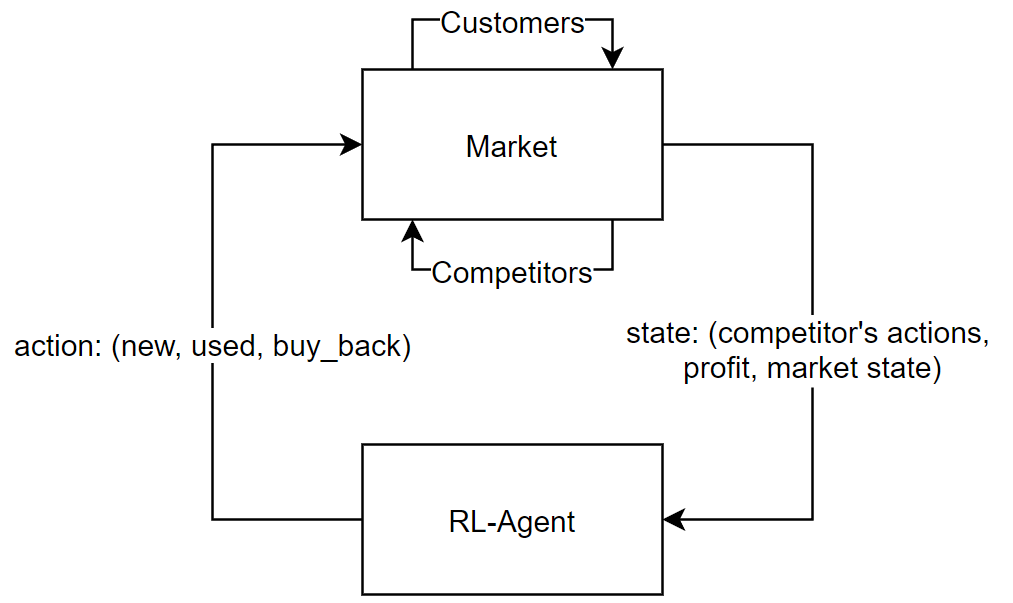
\includegraphics[height = 7 cm]{images/RL-Overview.png}\\[1 ex]
	\caption{The standard reinforcement-learning model in the context of our market.}
	\label{fig:IntroRLDiagram}
\end{figure}

Reinforcement-learning agents are trained through a process of trial-and-error. They interact with the market through an observable state and an action which influences the following state. \Cref{fig:IntroRLDiagram} illustrates the RL-model in the context of our market.\todo{re-buy instead of buy-back in the diagram}\todo{Create a \emph{nicer} diagram with the three prices} The goal of the agent is to maximize its reinforcement signal, which in our case is the profit the agent made during the last episode, since we want to train agents to maximize profits on real markets. An episode consists of a fixed, configurable number of timesteps, where in each step each vendor (agent) sets their prices and customers make purchasing decisions. By observing which prices lead to which profits (reinforcement signal), the agents get more effective in their pricing decisions over the course of training.

\chapter{Related Work}
\begin{jointwork}\label{ch:RelatedWork}
	This chapter will outline approaches to modelling and simulating recommerce marketplaces. Additionally, traditional and novel approaches to monitoring and evaluation RL agents on these marketplaces will be presented.
\end{jointwork}

\section{Dynamic Pricing Simulations}

The topic of dynamic pricing techniques is well explored, with the earliest mathematical models having been developed over a century ago \cite{DynamicPricingHistory}. With the emergence of e-commerce and the ability to cheaply and quickly change prices, as well as the freedom of information, including being able to know competitor's prices in real time, the topic has gained importance even further. However, research concerning dynamic pricing in e-commerce, especially in highly competitive markets, has not grown at the same pace~\cite{PricingEcommerceGrowth}. On the other hand, the role that autonomous agents will play in this new market environment, both in the form of vendors and customers, has for a long time been a topic of discussion and speculation alike~\cite{PricingBySoftwareAgents}. Dynamic pricing methods come in many different shapes and forms, from simple greedy algorithms over customer-choice methodology to machine-learning models \cite{deGeerPricing}. Due to this high number of options to choose from, and to enable researchers to evaluate their algorithms' performance, a unified platform for comparison is needed. The real market is not really an option for this, as it is near impossible to create equal opportunities for each pricing method to be able to reliably compare them to each other. This is one of the major reasons for simulating the real market - development, testing and comparison of new pricing methods.

% Nowadays, another market dimension is creating new challenges for businesses: Circular Economy models (see \bfref{sec:CircularEconomy}) which include two or more prices per product make it hard to price items manually using pricing experts or even regular dynamic pricing models, which may not be able to correctly adapt to interdependencies between prices. This is creating a demand for dynamic pricing methods using self-learning technologies, such as RL. And again, to train, test and evaluate such pricing agents, simulated environments are needed. In the case of RL, this is not only optional but required, as RL agents need to learn how a market environment works and how to interact with it before they become viable for use on the real market, as the pricing decision they take early on in the training process lack any experience and are therefore taken randomly, until enough knowledge about the market was collected.\todo{Judith: `Diesen letzten Absatz verstehe ich nicht so ganz. Hast Du das mit der CE nicht in dem 1.2 Genauso erklärt? Dann könntest Du hier den ersten Satz des Absatzes deutlich kürzen, bzw. Den kannst Du sowieso nochmal Teilen. Warum motivierst Du hier RL? Würde das nicht besser in das RL Kapitel passen? '}

\section{Visualization - State-of-the-art}

The process of training RL agents for any kind of task comes with the requirement for visualizing the data collected during training. This allows for an analysis of an algorithm's performance and gives insights into its strengths and weaknesses.

For the past years, going back as far as 2018, one of the most used frameworks overall and the most used for machine learning was TensorFlow~\cite{StackOverflowSurvey}. Aside from its API for model building, TensorFlow also provides a front-end visualization toolkit called TensorBoard, which can be used independent of other TensorFlow tools. TensorBoard provides an API for tracking and visualizing important metrics such as loss and accuracy, and allows developers to easily integrate their own metrics as well. During an experiment, data can be visualized live during the training process, allowing developers to quickly gain insights into the performance of the algorithms. In our recommerce market simulation framework, we use the TensorBoard in conjunction with our own tools for data visualization, see \cbfref{ch:Approaches}.

\section{Visualization - Novel approaches}

\subsection{Model visualization}

Aside from visualizing results of a training run, developers may also want to visualize the model itself. Tools such as the \emph{Graph Visualizer}~\cite{GraphVisualizer} are a step in the right direction, but the study found that while developers are satisfied with the visualization tool itself, they would prefer to be able to edit and influence the graph model directly. The \emph{SimTF} tool developed by Leung et al.~\cite{NeuralNetworkVisualization} attempts to solve this problem. The same as the \emph{Graph Visualizer}, the \emph{SimTF} tool is based on TensorFlow. The authors describe it as a \emph{library for neural network model building}. \emph{SimTF} acts as a middleman between the visually constructed neural network graph model and the TensorFlow API, allowing developers to modify the visualized model to influence the training network.

In our simulation framework, the used neural network model itself is quite static, users can only choose from a pre-set selection of network sizes, and all changes to hyperparameters must be done through configuration files ahead of a training run.

\subsection{Evaluation}

On the other side of the visualization tools we have those which provide insights into currently running or completed training runs, such as the previously mentioned \emph{TensorBoard}. Besides simply visualizing different collected data, the goal of most of these tools is to allow the developers to get a sense of the trained algorithm's performance, and to evaluate and compare it against previously trained agents using the same algorithm or other algorithm's completely.

When developing new algorithms, the most common barrier to proper comparison with current state-of-the-art algorithms is a lack in reproducibility of results. Benchmark environments such as those provided by OpenAI Gym \cite{OpenAIGym} lower this barrier by providing unified interfaces against which many algorithms have already been tested. However, the effects of extrinsic factors (such as hyperparameters) and intrinsic factors (such as random seeds for environment initialization) make proper, reliable reproducibility a challenge, something for which current evaluation practices do not account for~\cite{DRLThatMatters}. Jordan et al.~\cite{EvaluatingPerformance} propose a new, \emph{comprehensive evaluation methodology for reinforcement learning algorithms that produces reliable measurements of performance}. The authors describe the goal of their new evaluation technique as not trying to find methods (algorithms) that maximize performance with optimal hyperparameters, but rather to find those that do not require extensive hyperparameter tuning and can therefore easily be applied to new problems. This leads to a preference for algorithms that are not aimed at being the best at problems which are already solved (which applies to the aforementioned benchmark environments), but instead those which are most likely to succeed in new, unexplored environments.

\chapter{Simulating the marketplace}
\begin{jointwork}\label{ch:SimulatingMarketplace}
	In this section we will outline the requirements and challenges of transferring the vast amount of features and parameters that influence vendor and customer decisions in real recommerce markets to our simulated market environment. We will take a brief look at different market scenarios as well as how our customers work, with a focus on the unique feature of recommerce markets; the buyback of used items by the vendors. The focus of this chapter will however lie on the vendors, the Rule-Based as well as the ones trained using Reinforcement-Learning, comparing their features and how they fare against each other. These comparisons will be done using our various monitoring tools, which will be explained in the following chapter, \fullref{ch:Approaches} and put to use in \fullref{ch:AnalysingGraphs}. For further information on the overall framework structure refer to \cite{LeoThesis}, for detailed insights into our market processes, see \cite{NickThesis}.\todo{Rework start of this parapgraph}
\end{jointwork}

\section{Market scenarios}\label{sec:MarketScenarios}

In our framework, we implemented a number of `market blueprints' for classic Linear Economy markets as well as for Circular Economy markets both with and without rebuy prices enabled. There are marketplaces available for each combination of the following two features:
\begin{enumerate}
	\item Marketplace type: Linear Economy, Circular Economy, Circular Economy with rebuy prices
	\item Market environment: Monopoly, Duopoly, Oligopoly
\end{enumerate}
The marketplace type defines the number of prices the vendor has to set. In a Linear Economy, vendors only set prices for new items, in a Circular Economy prices for refurbished items need to be set as well. In order to simulate a recommerce market, the user can choose a Circular Economy with rebuy prices. The market environment defines the number of competing vendors in the simulation: Monopolistic and competitive markets are available, where the Duopoly is simply a particular version of an Oligopoly. Depending on the chosen market environment, one, two, or any number of vendors can be chosen to be used in the experiment. \Cref{fig:OverviewDiagram} shows a reduced overview of the classes in our framework which concern themselves with the market simulation, and how they interact with each other during the simulation.

In the most common use case of our framework, the training of Reinforcement-Learning agents, only the agent (or multiple agents in the case of training multiple Reinforcement-Learning agents against each other) that is to be trained needs to be configured by the user, as each market environment is equipped with a pre-defined set of competitors that will play against the agent defined by the user. To allow for more control over the simulation, users are however also able to change these competitors to use any vendors they want - as long as they are a valid fit for the marketplace type and the number of competitors chosen matches the market environment.

\begin{figure}[t]
	\centering
	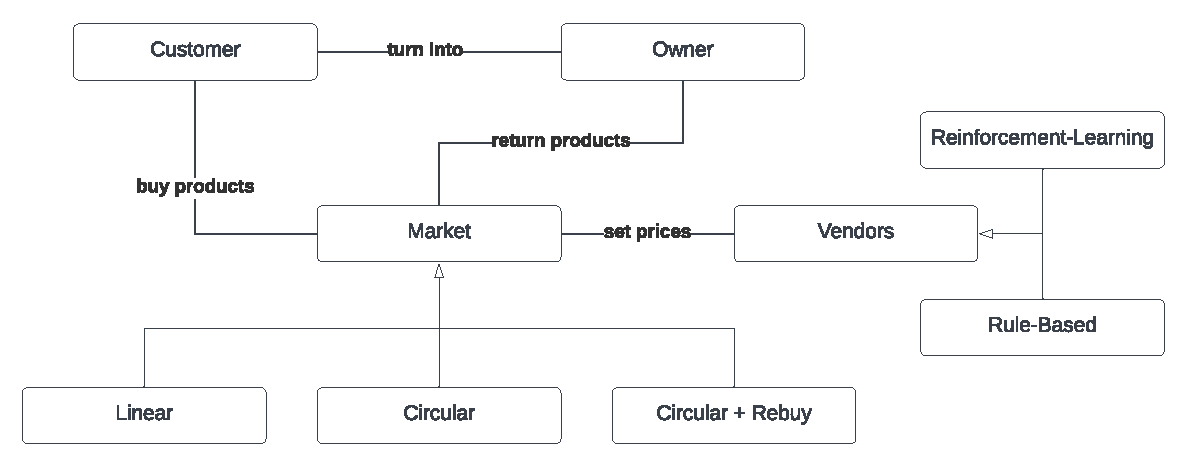
\includegraphics[width = \textwidth]{images/overview_diagram.pdf}\\
	\caption{Class diagram outlining interactions between classes concerning the market simulation.}\label{fig:OverviewDiagram}
\end{figure}

\section{Customers}\label{sec:Customers}

Customers are at the centre of every type of marketplace, which makes them an integral part of our market simulation. However, since each customer in the real market is an individual with different backgrounds and makes purchase decisions based on personal preferences, modelling a realistic depiction of real-world customers proves to be very difficult and time-consuming. For this reason we decided to keep our initial implementation of the customers as simple as possible, taking into account future extension and scalability concerns.

Most customers' behaviour can be classified into one of a (non-exhaustive) number of categories, such as \emph{Perfectionistic} or \emph{Impulsive} consumers, proposed in~\cite{ShoppingStyles} (also see \Cref{tab:shoppingStyles}). As we are focussing on dynamic pricing and our vendors can only change/influence the prices of their products, we decided on primarily building customers that value price over any other features a product may have, thereby incentivizing our vendors to make the most of their pricing power. This behaviour coincides with the shopping style of the \emph{Price Conscious} or\emph{Value for money} consumer.

\todo{Number of pages: I could remove this next paragraph, since we focus on Circular Economies}To make Linear markets a little more complex and add another dimension than just the \emph{new price} of a product for vendors to consider, random quality values are assigned to each vendor's products. Customers in this economy model were modelled to take this quality value into account when making their purchasing decisions, further reinforcing the shopping style mentioned above. As Circular Economy markets are inherently more complex than their linear counterparts (through the addition of two new price channels, which influence each other through their effect on customers), it was decided to remove the additional layer of quality values from these markets.

Within each simulated step, after the various vendors have set their prices, purchase decisions are made by the customers. To save on computational time, probability distributions are used to determine what part of the total number of customers will decide to take which action. See below for the way these distributions are calculated for an exemplary Circular Economy marketplace, for further information also see \cite{NickThesis}.

\begin{definition}\label{def:customerDecisions}
	Let \(P_{in}\) be the price of the new and \(P_{ir}\) the price of the refurbished product of vendor \(i\). Using these prices, for each vendor, we define \(R_{in}\) as the \emph{preference ratio} regarding \(P_{in}\):
	\[
		R_{in} := \frac{10}{P_{in}} - e^{P_{in} - 8}
	\]
	and similarly, \(R_{ir}\) as the \emph{preference ratio} regarding \(P_{ir}\):
	\[
		R_{ir} := \frac{5.5}{P_{ir}} - e^{P_{ir} - 5}
	\]
\end{definition}\todo{@Rainer @Alex: Should I add a graph for the preference ratios in the Appendix? AFAIK, Nick has one in his thesis, so I could also just leave it, as I already cited him.}

In order to be usable as a probability distribution, the different ratios need to add up to \(1\). We use \emph{softmax} to normalize our values, after which each \emph{preference ratio} will be within the interval \((0,1)\), with all ratios adding up to \(1\) as needed.

Following this, the market uses a \emph{multinomial} distribution to draw \(n\) samples, with \(n\) being the number of customers making a pruchasing decision in this step of the simulation.

As mentioned above, the current decisionmaking process of customers in our simulation is still quite basic. \fullref{sec:DivergingFromRealMarket} introduces a number of parameters and circumstances that can be used to make customer behaviour more realistic. Through the modular approach when building the framework, any customer behaviour implemented in the future can easily be added to the pool of available options, as long as it manifests in the form of a probability distribution, at which point the number of customers can be split between different distributions when drawing from the \emph{multinomial} distribution (or any other distribution if so desired).

\subsection*{3.2.1 Owners}

Once a customer has decided to buy a product from any of the available vendors, they turn into an \emph{owner}. In the next step of the simulation, they are offered the option of selling their now used product back to one of the vendors. If they decide to do so, the vendor pays them the advertised \emph{rebuy price} and adds the used product to their inventory, from where it can then be sold as a refurbished product in the next step.

In our simulation, all owners are memoryless, meaning that they do not remember the original price they paid for the product. Additionally, each vendor in the market is obligated to buy back any product, independent of the original vendor. In each step, every owner has the option to either keep the product for another step, discard it (meaning it is removed from circulation and not sold back to a vendor), or sell it to any one of the vendors in the market. Similarly to the way we compute customer purchasing decisions, the decisions owners take are also represented through probability distributions. When deciding if and to which vendor a product should be sold, the following formula is used:

\begin{definition}\label{def:ownerDecisions}
	We keep the variables defined in \Cref{def:customerDecisions}. Additionally, let \(P_{ib}\) be the price at which vendor \(i\) is willing to buy back an owner's product. For each vendor, we define \(P_{im}\) as the purchase option with the lowest price:
	\[
		P_{im} := \min(P_{in}, P_{ir})
	\]
	We define the likelihood \(R_{ib}\) that the owner will return their product to vendor \(i\) as follows:
	\[
		R_{ib} := 2 \cdot e^{(P_{ib} - P_{im}) / P_{im}}
	\]
	Additionally, the owner's \emph{discard preference} \(R_{d}\) is updated for each vendor as follows:
	\[
		R_{d} := \min({R_{d}, \frac{2}{P_{ib}+1}})
	\]
	Meaning the owner is more likely to discard their product if rebuy prices are low across the board.
\end{definition}

\section{Vendors}\label{sec:ExplainVendors}

Vendors are the main focus of our market simulation. While our framework will not be able to reproduce all types of pricing models used in the real market, we strive to model as many different models as possible (and feasible in the scope of the project). Due to the modular nature of the framework, it is possible for users to easily create and add their own pricing strategies in the form of a vendor that can play on a market. This allows users to not only add other Reinforcement-Learning algorithms, but also to define new Rule-Based strategies. For this reason, we also do not restrict the usage of our monitoring tools to just Reinforcement-Learning agents, but allow users to monitor any combination of vendors.\todo{@Rainer @Alex: Do I need to further motivate \emph{why} we allow this?}

We will use four types of dynamic pricing models, as defined in `Dynamic pricing models for electronic business'~\cite{dynamicPricingModels}, to describe the different models we implemented in our framework. These categories are not mutually exclusive, and many agents belong to more than one category.

\subsection*{3.3.1 Inventory-based models}\label{subsec:InventoryBasedModels}

These are pricing models which are based on inventory levels and similar parameters, such as the number of items in circulation (items which are currently in use by customers). In our framework, almost all Rule-Based agents consider their inventory levels when deciding which prices to set. The only exception to this rule are the simplest of our agents, the \emph{FixedPriceAgents}, which will always set the same prices, no matter the current market state and competitor actions. The prices these agents will set are pre-determined through the user's configuration of the experiment, and will not change over the course of the market simulation.

Inventory-based models are comparatively easy to implement, as they only depend on data immediately available to the vendor. This has the advantage that Rule-Based agents which fall into this category are relatively simple to create and modify. Examples of \emph{Inventory-based agents} in our framework can be found in the \emph{RuleBasedCERebuyAgent}, one of the first Rule-Based agents we created. This agent does not take pricing decisions of its competitors in the market into account, but simply acts according to its own storage costs, always trying to keep a balance between having enough (refurbished) products to sell back to customers and keeping storage costs low. It does this by checking into which of four possible ranges the current number of stored products falls. The more products the agent already has in storage, the lower it sets the rebuy price (to `prevent' customers from returning more products), and the lower it sets the price for refurbished products, to empty the storage more quickly and prevent high storage costs. While its performance is not necessarily bad, it is still one of the weakest competitors currently available in the framework. For the full implementation logic of the agent's policy, see \Cref{fig:PolicyRuleBasedCERebuy}. For a comparison of the \emph{RuleBasedCERebuyAgent} with a more sophisticated \emph{Data-driven model} see \Cref{fig:RulebasedAgentMonitoring}.

\subsection*{3.3.2 Data-driven models}\label{subsec:DataDrivenModels}

\emph{Data-driven} models take dynamic pricing decision-making one level further. They utilize their knowledge of the market, such as customer preferences, past sales data or competitor prices, to derive optimal pricing decisions. Aside from the aforementioned \emph{FixedPriceAgents} and the basic \emph{RuleBasedCERebuyAgent}, all of our other Rule-Based agents fall into this category. One of the most prominent examples of a \emph{Data-driven model} is the \emph{RuleBasedCERebuyAgentCompetitive}, an agent whose basic goal is to always try and undercut competitor prices, while also keeping track of the current amount of items in storage. In its policy, this agent first always undercuts the new price of all other competitors. Then, similar to the \emph{RuleBasedCERebuyAgent}, the agent looks at the current amount of stored products and depending on the range, sets lower prices for refurbished items and higher rebuy prices, while always trying to give customers a better deal than any of the competitors. Again, the full implementation logic of this vendor's policy is available in the Appendix, under \Cref{fig:PolicyRuleBasedCompetitive}.

Notably, all of our \emph{Data-driven models} are also \emph{Inventory-based} to a certain extent, as handling storage plays a big part in a Circular Economy market setting, where used products need to be bought back from customers and subsequently undergo refurbishment while in inventory of the company. \emph{Data-driven models} have proven to be the most competent Rule-Based agents in our recommerce market scenario, in particular the above described \emph{RuleBasedCERebuyAgentCompetitive}, which is able to outperform most other Rule-Based agents, both \emph{Inventory-based} and \emph{Data-driven models} (please refer to e.g. \Cref{fig:PPOOligopolyLineProfitsAll}).

\subsection*{3.3.3 Game theory models}\label{subsec:GameTheory}\todo{Number of pages: If any section needs to be removed here (e.g. for page length), this should be the one}

Game theory concerns itself with the study of models for conflict and cooperation between rational, intelligent entities~\cite{GameTheory}. It is therefore often applicable in situations where competing individuals, acting rationally and selfishly, interact with each other. In our framework, most competitors in the market are influenced in their decision-making processes by the actions of other participants of the scenario. This is especially true for the Reinforcement-Learning agents, which base their policy on the received market states, which include their competitor's actions. While none of our Rule-Based agents have been specifically designed to act according to game theoretic strategies, due to the fact that almost all of them consider their competitors prices in their pricing decision, and due to the nature of Reinforcement-Learning trying to maximize their own profits without regard to their competitors performance, behaviour according to Game theory can sometimes be observed. This can be observed especially well in the beginning of training sessions, where Rule-Based competitors often struggle to achieve high profits while the Reinforcement-Learning agent is making great losses, but are then able to increase their profits as the trained agent starts to make better decisions as well. Many examples of such behaviour can be found in the diagrams shown in \fullref{ch:AnalysingGraphs}, such as in \Cref{fig:SACDuopolyProfitsMean}.

During training, Reinforcement-Learning agents observe the market state, which includes prices and sales data not only of themselves but also the other vendors in the market. Using this data, the algorithms try to predict how their prices will influence customer behaviour as well as the competing vendors. In some cases, depending on the concrete behaviour of the competitors, vendors may cooperate in driving prices higher together, in other cases the agents may act seemingly irrationally, lowering prices in order to force their opponents to lower theirs as well. An example of such behaviour can be seen in the development of prices for new items set by the two competing vendors in \Cref{fig:SACDuopolyMixedGraphs4}.

\subsection*{3.3.4 Machine learning models}\label{subsec:MachineLearningModels}

All of our Reinforcement-Learning agents fall into this category. As they are not the focus of this thesis, we will not go into detailed explanations of the various models used. For a comparison of the performance of different Reinforcement-Learning algorithms in the context of our simulation framework, please refer to~\cite{JanThesis} The following will give a short overview over the different algorithms used in our framework.

There are two `origins' of the algorithms in our framework. In the earlier phases, \hyperref[item:QLearning]{Q-Learning} and \hyperref[item:ActorCritic]{Actor-Critic} algorithms were custom implemented by us. Later on, we used the \hyperref[item:StableBaselines]{Stable-Baselines} library to incorporate a greater number of pre-implemented algorithms into our framework. While these are not as easily configurable, they can quickly be used without much additional work.

\begin{itemize}
	\item \phantomsection\emph{Q-Learning}:\label{item:QLearning} \emph{Q-Learning} agents were the first Reinforcement-Learning agents we introduced in our framework, as its algorithm is one of the easier ones to implement~\cite{reinforcementLearningOverview}. The \emph{Q-Learning} algorithm used in our framework is implemented using the \emph{pytorch} framework (see \cite{Pytorch}). However, the drawback of using \emph{Q-Learning} in our framework is that it can only be applied to discrete action and state spaces. This means that when using \emph{Q-Learning}, only `whole' prices can be set by our vendors, and any decimal places must be omitted. This of course limits the framework in its realism, as the fine-tuning of prices using decimal places can be critical in influencing customer decisions. In the initial exploration-phase of our simulation framework this was not a problem, as relatively small action spaces were used, adapted to this limitation. But by now, our simulation framework also supports continuous action and state spaces, to allow more complex algorithms such as those introduced in the sections below to function. While approaches for \emph{Q-Learning} algorithms that can work with continuous action and state spaces have been presented in the past (\cite{QLearningContinuous},~\cite{QLearningContinuous2}), we have chosen not to implement such an algorithm in our framework, but rather explore approaches other than \emph{Q-Learning}, such as \emph{Actor-Critic} algorithms, introduced below.

	\item \phantomsection\emph{Actor-Critic}:\label{item:ActorCritic} \emph{Actor-Critic} algorithms are more complex than Q-Learning algorithms, and have therefore been implemented later in the process. They are structured different then Q-Learning algorithms in the way that they are `split' into two parts: The \emph{actor} is responsible for selecting actions, while the \emph{critic} is responsible for critiquing  the actions taken by the \emph{actor}, thereby improving its performance~\cite{ActorCritic}. Similar to the \emph{Q-Learning} agents, the \emph{Actor-Critic} algorithms have also been implemented by us. In total, one discrete and two continuous \emph{Actor-Critic} agents can be used, in addition to those provided through \emph{Stable-Baselines}, see the next section.

	\item \phantomsection\emph{Stable-Baselines}:\label{item:StableBaselines} Stable-Baselines provides a number of open-source implementations for various Reinforcement-Learning algorithms. In our framework, we use the latest version of these algorithms, through \emph{Stable-Baselines3} \cite{StableBaselines3}. The advantage when using algorithms provided through Stable-Baselines lies in the fact that they need close to no custom implementation from our end, we can instead interact with them through very simple interfaces. This cuts down on the amount of time and effort that needs to be spent developing, implementing and maintaining these powerful algorithms, and allows us to introduce a higher number of algorithms than would otherwise be possible. Currently, five different \emph{Stable-Baselines3} algorithms are used in our simulation framework, see the \emph{Stable-Baselines3} documentation~\cite{StableBaselines3Algorithms} and the referenced papers for more information about the different algorithms:
	      \begin{itemize}
		      \item \emph{A2C}: Advantage-Actor-Critic (\cite{StableBaselines3A2C})
		      \item \emph{DDPG}: Deep deterministic policy gradient (\cite{StableBaselines3DDPG})
		      \item \emph{PPO}: Proximal Policy Optimization (\cite{StableBaselines3PPO})
		      \item \emph{SAC}: Soft Actor-Critic (\cite{StableBaselines3SAC})
		      \item \emph{TD3}: Twin-delayed deep deterministic policy gradient (\cite{StableBaselines3TD3})
	      \end{itemize}
	      We will be using some of these algorithms in our experiments and briefly compare them with our Rule-Based approaches using our various monitoring tools, which are introduced in the next chapter, \fullref{ch:Approaches}.
\end{itemize}


\chapter{Approaches to monitoring agents}
\begin{jointwork}\label{ch:Approaches}
	In this chapter, we will take a look at the different approaches we took to monitoring agents in our framework, explaining the reasons why we chose to implement specific features and how they help us in determining an agents strengths and weaknesses.
\end{jointwork}

\section{When to monitor what}\label{sec:WhenToMonitorWhat}

Our \emph{workflow} (which will be explained in more detail in \cbfref{ch:OurWorkflow}) can generally be split into two parts when it comes to monitoring and evaluating agents: \emph{during} and \emph{after} training. When talking about the \emph{workflow} we refer to the process of configuring and starting a training session, where an RL agent is being trained on a specific marketplace against competitors. The \emph{workflow} also includes the subsequent collection of data used to evaluate an agent's performance. We are also introducing the term of the \emph{complete agent} in this section, which will be used to refer to both RL agents that have completed a training run, and rule-based agents which do not need training.

As mentioned above, we split our monitoring tools into the following two categories:

\begin{enumerate}
	\item \textbf{During training} (\bfref{sec:DuringTraining}): Having data available as soon as possible without having to wait for a long training session to end is crucial to an efficient workflow. Our framework enables us to collect and visualise data while a training session is still running. This allows users to always be well-informed about the currently running experiments. In some cases, when an agent's performance is severely lacking, users may want to stop a training session before it has finished, which is enabled through these monitoring tools. We also include the \emph{Live-monitoring} tool in this category, which runs directly after a training session has finished, see \bfref{subsec:LiveMonitoring}.

	\item \textbf{On complete agents} (\bfref{sec:CompleteAgents}): After a training session has finished we have a complete and final set of data available for an agent, which enables us to perform more thorough and reliable tests. These can include simulating runs of a marketplace to gather data on the agent's performance in different scenarios and against different competitors, or running a static analysis of the agent's policy in different market states. The tools available for trained agents are in the same way also usable on rule-based agents.
\end{enumerate}

In the following sections, we will take a look at the tools our framework provides for monitoring agents, distinguishing between the two general types of monitoring mentioned above. The goal of these sections is to give a short overview of each tool, how and why they were implemented and what value they offer to the framework as a whole. We will also discuss some features that are not yet available, explaining how they could benefit the entire workflow and enrich the overall experience.

\section{Monitoring during training}\label{sec:DuringTraining}

When talking about monitoring agents during a training session, we are always referring to RL agents, as rule-based agents always perform the same and cannot be trained. But even though they cannot be trained, our monitoring tools listed in the next section, \bfref{sec:CompleteAgents}, can still be applied to rule-based agents as well, as users may want to compare different rule-based strategies against each other, or measure the strategy's performance on a market before training an RL agent.

Monitoring agents while they are still being trained enables us to be more closely connected to the training process. Ultimately, the goal of such monitoring tools is to be able to predict the estimated `quality' of the final trained agent as reliably as possible while the training is still going.

\subsection{TensorBoard}\label{subsec:TensorBoard}

The \emph{TensorBoard} is an external tool from the RL library \emph{TensorFlow}~\cite{TensorFlow}. With just a few lines of code a training session can be connected to a TensorBoard instance. We are then able to pass any number of parameters and metrics we deem interesting or useful to the TensorBoard, which then offers visualisations for each of them, updating live as the training progresses. In addition to metrics specific to our market simulation, which can be found in \Cref{tab:AllMetrics}, the TensorBoard also visualises a number of specifically training-related data points, such as the number of episodes simulated per second. To access these web-based visualisations, a local server needs to be started. The diagrams created using the TensorBoard are an immensely useful tool for quickly and easily recording data and offering a first rough comparison of competitors in the market. Aside from simple visualisations, TensorBoard also offers many plugins, and even enables users to write their own~\cite{TensorBoardPlugins}. Plugins such as the \emph{What-If Tool} \cite{WhatIfTool},~\cite{WhatIfToolWeb}, which allows users to feed trained models with hypothetical situations to study their behaviour, can have a great influence on the way users interact with the TensorBoard and their machine learning models.

\subsection{Live-monitoring}\label{subsec:LiveMonitoring}

Unlike the TensorBoard, the monitoring tools summarized under the term \emph{Live-monitoring} were completely and from the ground up built by our team. For most of the visualisations, the \emph{matplotlib}~\cite{Matplotlib} library was used. The Live-monitoring tool combines two use cases: First, it creates visualisations for all data recorded during the training, similar to those provided through the TensorBoard. This needs to be done to be able to access the visualisations even after the training has concluded, as the TensorBoard relies on abstract data files for its visualisations. By taking the data we have at the end of the training and using our own visualisation tool, we create two types of diagrams: Scatterplots, which contain all samples for a certain parameter (see for example \Cref{fig:SACDuopolyMixedGraphs3}) and lineplots, which show smoothed data, such as it would be available in the TensorBoard (see for example \Cref{fig:SACDuopolyProfitsMean}). Secondly, the tool simulates a market scenario identical to the one used during training an additional time. To understand why we do this, we need some additional information: During a training session, `intermediate' models, as we will call them, are being saved in regular intervals. These models contain the current policy of the agent and can be used the same as any other model of complete agents, the only difference being the quality of the agent, which can change over the course of a training run, both for the better and worse. These intermediate models can then be used by a range of monitoring tools available to us. Since the models only contain the current policy of an agent but not the history of states and actions preceding the model, we need to run separate simulations on these models to be able to analyse and evaluate them. For this, we utilize our \emph{Agent-monitoring} toolset (explained in detail in \bfref{subsec:AgentMonitoring}). In \bfref{subsec:LiveMonitoringResults} we will discuss the results of a training session using the Live- and Agent-monitoring tools.

\section{Monitoring complete agents}\label{sec:CompleteAgents}

For monitoring trained RL and rule-based agents, we offer three major tools: The Agent-monitoring tool allows users to simulate a large number of episodes to visualise bigger trends, the Exampleprinter simulates a single episode, offering detailed insights into market states using an overview diagram, and the Policyanalyser is a static tool which can be used to analyse a vendor's reaction to different market states and competitor actions.

\subsection{Agent-monitoring}\label{subsec:AgentMonitoring}

\begin{figure}
	\centering
	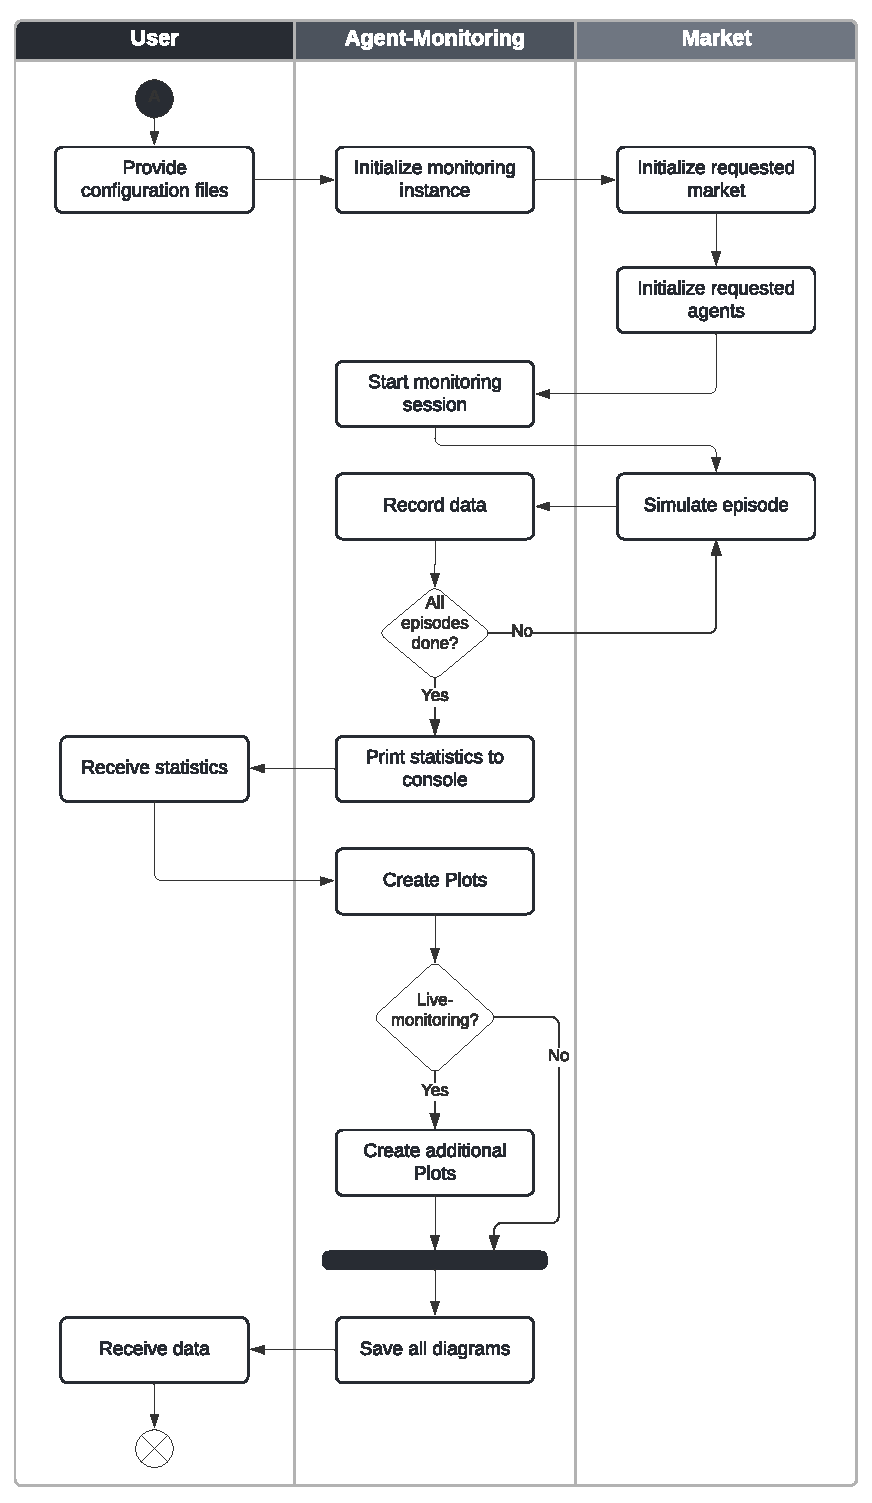
\includegraphics[height = 0.9\textheight]{images/swimlane_monitoring.pdf}\\
	\caption{The internal workflow when running an Agent-monitoring session. \Cref{tab:AllMetrics} lists the different types of diagrams created by both the Live- and Agent-Monitoring, and which of the recorded metrics they visualise.}\label{fig:SwimlaneMonitoring}
\end{figure}

The \emph{Agent-monitoring} is a highly configurable tool for monitoring and evaluating different combinations of agents and marketplaces. \Cref{fig:SwimlaneMonitoring} shows how the tool works internally.

In addition to parameters provided to the marketplace and monitored agents, the following parameters can be used to configure the \emph{Agent-monitoring} tool itself:

\medskip
\noindent\textbf{Episodes}: This parameter decides how many independent simulations are run in sequence. At the start of each episode, the market state will be reset and randomized. Within an episode, the vendors run through a configurable amount of time steps, during each of which they set prices (depending on the chosen economy type, this can range from only one price for new items to three prices, including a rebuy price for used items) and a set number of customers interact with them.

\medskip
\noindent\textbf{Plot interval}: A number of diagram types enable the user to view averaged or aggregated data over a period of time. The plot interval parameter decides the size of these intervals. Smaller intervals mean more accurate but also more convoluted data points. Computational time also increases with a smaller interval size.

\medskip
\noindent\textbf{Marketplace}: Using this parameter, the user can set the marketplace on which the monitoring session will be run. Refer to \bfref{sec:MarketScenarios} for an explanation of the different available marketplaces.

\medskip
\noindent\textbf{Separate markets}: This parameter is a boolean flag that determines the way in which the monitoring session will handle the agents given by the user. If the flag is enabled, each agent will be initialized on a separate instance of the chosen marketplace, meaning that the agents will be monitored independent of each other. This functionality takes a lot longer than if the flag were disabled, as the whole marketplace is simulated once for each agent. While it may seem like the same results could be reached by simply starting multiple monitoring sessions with a different agent each, this is not the case. Using this flag instead, it is ensured that all agents get the exact same market states for each episode. By running multiple marketplaces in parallel using the \emph{separate markets} flag, we can match the simulations as closely as possible. The most prominent use case where this flag is enabled is during the Live-monitoring after a training session, where all intermediate models are being monitored on separate markets.

If the flag is disabled, the monitoring tool will initialize only one marketplace and set the passed agents to directly compete against each other on this marketplace. This functionality is most useful when monitoring only a single agent, trying to determine its specific strengths and weaknesses against certain opponents, as it will complete a lot faster than if the flag were enabled.

\medskip
\noindent\textbf{Agents}: Depending on the chosen marketplace, only a select number of agents can be chosen to be monitored, as each agent is built to interact with a specific type of marketplace. First off, all agents belong to one of the two major categories: \emph{RL agent} or \emph{rule-based agent} (for a more detailed overview see \bfref{sec:ExplainVendors}). RL agents can only be monitored on the marketplace type and market environment they were trained on, as these define the number of inputs and outputs the agent expects. Rule-based agents can only be used on the marketplace type they were built for, as each of them makes assumptions about the number of prices they will need to set, but the market environment may be freely chosen. This leads to not all marketplace types having the same amount of rule-based vendors available. Following their importance for our simulation framework, the Linear Economy has the least and most often weakest vendors available, while the more refined competitors are most of the times only available as a version compatible with the Circular Economy with rebuy prices.

\medskip
During each episode and for each vendor, all market events are being recorded. At the end of the monitoring session, the collected data is evaluated in different visual formats. First of all, all data that would be available to see in the \emph{TensorBoard} during a training session is visualised using density plots. These plots can be used to compare the vendors in a more granular way, if for example the effect of a parameter on the customer's sell-back behaviour of used items should be tested. Another visualisation that is created is a histogram containing the cumulative profits per episode for each agent, plotted against each other (see for example \Cref{fig:PPOOligopolyCumulativeRewards}). This allows for a quick overview to see which agent had an overall better performance. One additional type of diagram is only created if the Agent-monitoring is run through the Live-monitoring tool: Violinplots. These plots, which are created for all data points available through TensorBoard (also see \Cref{tab:AllMetrics}), depict distributions using density curves, accentuating the minimum, maximum and median values. Violinplots are used by us to compare different training stages of an agent, as small policy changes can have great impact on these values. For exemplary Violinplots created after training, see \Cref{fig:SACDuopolyViolinPlots}.

Aside from monitoring after a training session, a common use case of the \emph{Agent-monitoring} tool is to test trained agents against competitors other than the ones it was trained against. This is done to test the agent's capacity to adapt to different circumstances, an important factor in deciding an agent's quality, as its competitors in the real market will differ from any it has encountered in training, due to the sheer vastness of options when it comes to dynamic pricing models available nowadays. %, see \bfref{sec:ExplainVendors}.

\subsection{Exampleprinter}\label{subsec:Exampleprinter}

The \emph{Exampleprinter} is a tool meant for quickly evaluating a market scenario in-depth. When run, each action taken by the monitored agents is being recorded, in addition to market states and events such as the number of customers arriving and the amount of products thrown away. At the end of this quick simulation an animated overview diagram is created, which shows all actions and their consequences for each step in the simulation, see for example \Cref{fig:SACDuopolyExampleprinter17}. Due to the large amount of data that is being collected and visualised and the overhead would come with doing so for hundreds of episodes, we chose to disconnect this functionality from large-scale tools such as the Agent-monitoring. While the Agent-monitoring tool could be seen as a tool that imitates Macro-economic behaviour, simulating hundreds of days through hundreds of episodes, the Exampleprinter instead simulates only one day, recording and visualising all data collected during that time.

\subsection{Policyanalyser}\label{subsec:Policyanalyser}

The last tool we want to introduce is the \emph{Policyanalyser}. The \emph{Policyanalyser} is our only tool which does not simulate a market. Instead, the tool can be used to monitor an agent's reaction to different market states. The user can decide on up to two different features to give as an input, such as a competitor's new and refurbished prices, and the Policyanalyser will feed all possible input combinations to the agent and record its reactions. When initializing the \emph{Policyanalyser}, the user defines a number of parameters: The agent whose policy should be analysed, as well as the marketplace and the competitors that should be used, just as is done for all the other tools. Additionally, the user defines a \textbf{template market state}, a market state containing all values that are passed to the analysed agent, such as the number of items currently in circulation and the prices of competitors. Lastly, a list of \textbf{analysed features} needs to be provided, which defines one or two features of the template market state that should be varied. When the \emph{Policyanalyser} is run, these features are inserted into the template market state, overwriting the initial values and creating a new combination. This new market state is then passed on to the \texttt{policy}-method of the analysed agent (example policies of some of our rule-based agents can be found in \bfref{sec:AppendixPolicies}), and its reactions are recorded and visualised. See \bfref{subsec:ResultsPolicyanalyser} for use cases of this tool.

The \emph{Policyanalyser} is the monitoring tool which operates on the smallest scale out of all the tools we built for our framework. It allows users to define any market state they want and to then accurately monitor a vendor's reactions to changes to this specific state. While the tool can just as well be utilized to test new rule-based strategies, it is very much meant to be used as a way to understand RL agents better, as their policies are not immediately visible to the end-user and must therefore be discovered through tools such as the one's we built.


\chapter{The \emph{recommerce} workflow}
\begin{jointwork}\label{ch:OurWorkflow}
	The main goal of the market simulation framework is to provide a simple-to-use but powerful tool for training Reinforcement-Learning algorithms on highly configurable markets for users in both a research and a business context. To achieve this, multiple components had to be developed and connected to create the workflow we now provide. This section will introduce the most important parts of the workflow.
\end{jointwork}

When working with our simulation framework, users can choose from two options: First, it is possible to use our tool via a custom Command line interface (CLI). Alternatively, users can interact with the framework through a web-interface, which utilizes Docker for remote-deployment of tasks issued by the user. For detailed insights into our web-interface and remote deployment, see \cite{JudithThesis}.

\Cref{fig:WorkflowSwimlanes} depicts the common workflow activities in our framework. For all possible tasks, the user needs to provide configuration files, which define both the task to be worked on and parameters which influence market and agent behaviour (see \fullref{sec:ConfigureRun}). After the configuration files have been validated, the simulation framework initialized the requested marketplace and agents, and then starts the requested task, for which there are currently three options provided through the CLI or web-interface: \emph{Training}, \emph{Agent-monitoring} and \emph{Exampleprinter}. You may have noticed that one of our monitoring tools is missing from this list, the \emph{Policyanalyser}. As is mentioned in \bfref{subsec:FuturePolicyAnalyser}, this tool must unfortunately still be started manually by the user, as it has not been integrated into the rest of the workflow yet.

At the end of the respective task, the user is always provided with the various diagrams and data (e.g. trained Reinforcement-Learning models) collected during the respective task, which can then be used in subsequent tasks.

\section{Configuring the run}\label{sec:ConfigureRun}

\begin{figure}[t]
	\centering
	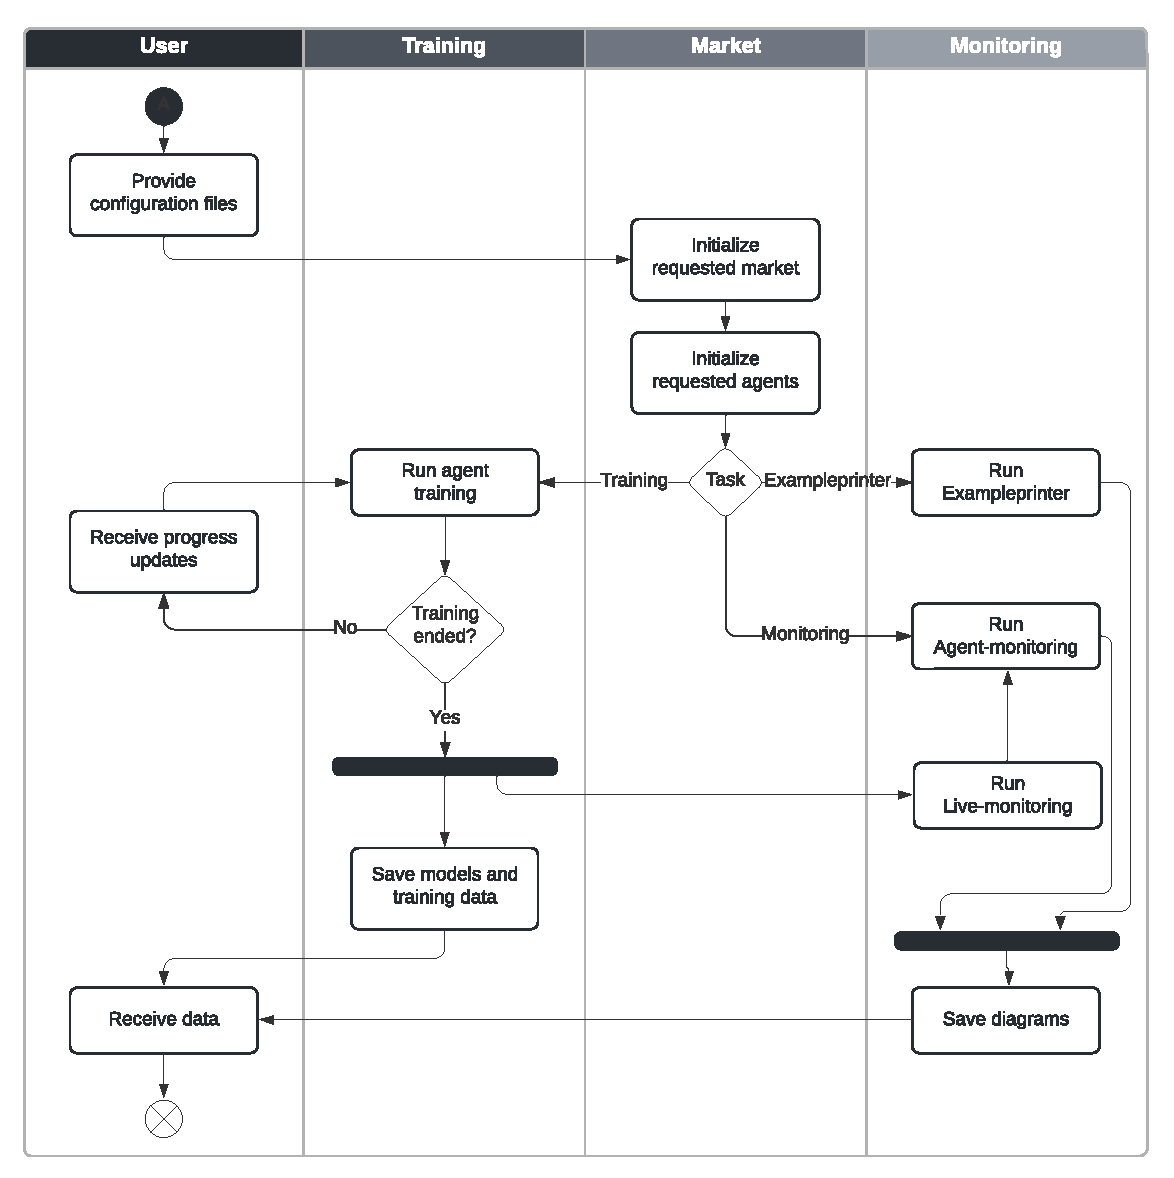
\includegraphics[width = \textwidth]{images/workflow_swimlanes.pdf}\\
	\caption{Diagram depicting possible workflows without webserver interaction.}\label{fig:WorkflowSwimlanes}
\end{figure}

Configuration is one of the most important aspects of the workflow. Without it, each simulation and training session would produce similar, if not the same results. By tweaking different parameters of a run, market dynamics can be changed and agent behaviour and thereby performance be influenced. The goal of our monitoring tools is to enable users to assess the extent to which each parameter influences certain characteristics of the training and/or monitoring session, and to enable them to make informed decisions for subsequent experiments.

Ultimately, all configuration is done using various \texttt{.json} files which contain key-value pairs of the different configurable items. We further differentiate between different groups of configurations, which means that hyperparameters influencing the market, such as maximum possible prices or storage costs, are being handled separate from parameters needed for Reinforcement-Learning agents, such as their learning rates, allowing users to easily change and tweak parameters involving different parts of the framework. Examples of such configuration files can be found in \Cref{fig:SACDuopolyConfigEnvironment} and \Cref{fig:SACDuopolyConfigMarket}.\todo{Just mention the seciton in Appendix}

% Our main goals when building our configuration tools were to make sure that users are able to quickly and safely configure their experiments in a way that is also easily reproducible. To be as user-friendly as possible, a lot of validation logic has been implemented to be able to catch invalid configurations as early as possible, making sure that whenever a training session is started, it is confirmed that the configuration is valid and the training will not fail due to wrongly set parameters at any point. Since our project has also been deployed to a remotely accessible, high-performant machine, we decided on creating an approachable web-interface for our configuration tools, which can now be used for both configuring, starting and evaluating experiments.

% \subsection*{The webserver/Docker-API}\todo{Judith: `Das ganze wie nutze ich die Konfiguration auf dem Webserver könntest Du meiner Meinung nach kürzer fassen'}

% \todo{Example screenshot of the webserver. Configuration and running page?}
% On our webserver, users can upload .json files containing any number of (valid) key-value pairs, or create configurations using a self-validating form, always making sure that it contains only valid values. For example, if the user chooses a Circular Economy market scenario with rebuy prices enabled, the user will not be able to configure agents that cannot operate on such a market.

% Aside from uploading or configuring complete, ready-to-go configurations, users can also choose to upload or create partial configurations, which can then be combined with other configuration objects to create a complete, valid configuration. This allows users to create multiple incomplete configurations containing only select parameters and then test all permutations of these configurations to observe the effect the different parameter combinations have on the experiment. \todo{Mention that this currently needs to be done manually, future work section?}

% An example of one such approach can be found below:
% \todo{Example of a mix and match of parameters}

% After having configured the experiment, the webserver also offers the option of starting multiple runs of the same configuration simultaneously. Most of the times this is recommended, as singular runs are prone to misleading results due to the trained agents training with specific market states, which in some cases may lead to behaviour unique to this starting configuration\todo{Example: Two completely different runs with the same configuration}. By running the same configuration multiple times using different starting circumstances for both the agent that is to be trained as well as its competitors, a configuration's effect on the agent's performance can be disconnected from the pseudo-random market states which influence the vendor's decision making processes.

%% This is regarding Reliability. Maybe I can re-use this in the Interpretation-Chapter, but since I removed it from the title/thesis focus, it is sort of too much for this section
% \todo{Is this perhaps too much interpretation for this section?}\todo{Alex: `Zu deiner Anmerkung: Du hast 2 Optionen um so etwas zu betrachten, entweder Mean + Standardabweichung oder Median + Quantile/Dezile bei sehr stark asymmetrischen Verteilungen. Was für deinen Use Case besser ist kann ich nicht ausm Stehgreif sagen ohne die Daten gesehen zu haben'} A configuration can be interpreted as producing `reliable' agents if any number of simulations all converge on similar agent performances (meaning similar mean rewards). The more singular runs diverge from the mean, \todo{mean or median? What do I use?}the more the agent's performance is dependent on the initial market state, meaning that its performance is less stable, as it will produce unpredictable results on new, unknown market scenarios. A higher number of runs that produce agents which perform on similar levels of performance means that the specific configuration, to be exact the parameters responsible for the Reinforcement-Learning algorithm, produces `reliable' agents: No matter the state of the market, the agent can always be expected to perform on the same level that was observed during the training process, setting prices that lead to similar profits. Reliability is therefore one of the most important factors in determing an agent's overall quality, as the ultimate goal is always to be able to deploy the agent onto the real market, which will always differ from the simulated environments the agent experienced during training, simply due to the fact that real markets are being influenced by so many more parameters than one could model in our, or for that matter any simulation framework. It should be noted that the chosen Reinforcement-Learning algorithm drives the reliability of a configuration, as many of the other hyperparameters most often have no impact on this aspect of an experiments results.

%% This section is very long but doesn't really add any useful information
% \section{Choosing what to show the user during training}\todo{Alex: `Die Struktur von 5.2 ist mir noch nicht ganz klar, aber da hört dein Draft ja auch auf, insofern ist das wohl harmlos'}

% During the training process, we of course record all actions the different vendors take, both for the training agent and its competitors, be they Reinforcement-Learning agents as well, or Rule-Based agents. Market states and events are also being recorded, to be able to match them to the agent's actions later on. Users of course want to have an indicator of how the training run is going so far, both to inform themselves about the total progress of the training, but also about the quality of the agent they are training. We now have to decide what information is shown to the user, making sure that the user is well informed, whilst also holding back on displaying too much information at once to prevent confusion, as the underlying data and states are ever-evolving, leading to many datapoints being invalidated shortly after their creation. This potential overflow of information is the reason why we decided on displaying minimal information to the user while the training session is still running: Training progress and current performance, in the form of the current overall mean profit.

% The first choice and a save bet when looking at datapoints that will be shown to users is the current training progress. Each training run is defined in its length by a parameter that sets the number of episodes that should be simulated. Each episode consists of an independently initialized market state on which a configurable amount of steps is run. Within each step, the vendors take turns in observing the current market state and then setting their prices for the new and refurbished products and depending on the chosen marketplace, a rebuy price.\todo{Should episodes and steps be defined/explained earlier than this? In the introduction? Specific section/Chapter for important terms and phrases?} We use the training progress to drive the frequency with which data is being shown to the user using the console: Every 10 episodes, we output the current progress, containing both the current number of steps and episodes completed, as well as the mean reward over all episodes the agent has completed. Additionally, to give a more visual component to the training progress a progress bar is displayed, which also tries to estimate the training-time remaining, based on the previous length the simulation of an episode took.

% Using only these two datapoints, the user knows the two most important things: How far along in the training process they are, and how the agent is currently performing.

% \todo{Small paragraph for rl-vs-rl and self-training having different output}

\section{The monitoring workflow}

Within the recommerce workflow, there are two points in time when our monitoring tools are or can be used. While a training session is running, the TensorBoard tool is automatically used to record metrics and give insights into the current training run, by creating visualizations of current market states. By saving intermediate models, the Live-monitoring enables the user to compare agent models saved at different times within the training process, after it has concluded. This can be especially useful when trying to determine the most effective amount of training steps after which a model does not improve further, to optimize future runs. After the training has finished, or at any point disconnected from a training session, our tools described in \fullref{sec:CompleteAgents} can be used to further analyse the trained models. If a training session is terminated by the user before it has completed, the Live-monitoring tool will not be run, but all intermediate models saved up to that point can still be used to monitor the agent's policy at that point in time. The next chapter, \fullref{ch:AnalysingGraphs}, is dedicated to the monitoring workflow, where we will first run a training session, and then monitor and evaluate the results we get from it.

% \subsection*{After training}

% As has been mentioned before, the end-goal of users using the simulation framework is to be able to deploy trained agents into real markets to set prices independent of human input or guidance. Starting from this premise, the goal of the training process is therefore to model the marketplace as realistically as possible, so that the trained agents can transfer the knowledge from their training to the real market `without noticing a difference'. Before deploying agents to the real market, they need to be tested on their reliability and robustness, to make sure that their policies are not just effective under certain circumstances, but that they are also able to adapt to different market scenarios and behave accordingly.

\chapter{Analyzing Graphs}
\label{ch:AnalyzingGraphs}

\begin{jointwork}
	In this chapter, we will put the tools and workflows described in the previous sections to the use. We will train a Reinforcement-Learning Agent, and then monitor it using all of the tools at our disposal, highlighting where each tool is most useful, and what could be improved.
\end{jointwork}

\section*{Setting up the experiment}

% Before starting our monitoring, we will be conducting two different experiments, each with a different Reinforcement-Learning algorithm and a different market environment. Both experiments will however be conducted on the same marketplace type, a Circular Economy model with rebuy-prices. To ensure that we are evaluating an agent with a performance that is to be expected with the provided parameters after the experiments have finished, we will run both the experiments multiple times to be able to identify outliers in the data. Diagrams of different versions of an experiment will be denoted using an underscore for differentiation.

% \subsection*{SAC-Duopoly}

% For the first experiment, we will train a Reinforcement-Learning Agent using the SAC-algorithm~\cite{StableBaselines3SAC} on a Duopoly marketplace with rebuy prices. The agent will be trained against a Rule-Based agent, more specifically the \emph{RuleBasedCERebuyAgentStorageMinimizer}, as presented in \nameref{subsec:DataDrivenModels}. The configuration files for this experiment can be found in \Cref{fig:SACDuopolyConfigEnvironment}, \Cref{fig:SACDuopolyConfigMarket} and \Cref{fig:SACDuopolyConfigAgent}. We will refer to this experiment as the \emph{SAC-Duopoly}.

%% Text from when there was only one experiment
Before starting our monitoring, we will need to conduct an experiment, where a Reinforcement-Learning algorithm is being trained on a market environment. For our experiment, we will train a Reinforcement-Learning agent using the SAC-algorithm~\cite{StableBaselines3SAC} on a Duopoly marketplace with rebuy prices. The agent will be trained playing against a Rule-Based agent, more specifically the \emph{RuleBasedCERebuyAgentStorageMinimizer}, as presented in \nameref{subsec:DataDrivenModels}. The configuration files for this experiment can be found in \Cref{fig:SACDuopolyConfigEnvironment} and \Cref{fig:SACDuopolyConfigMarket}. We will refer to this experiment as the \emph{SAC-Duopoly} experiment. To ensure that we are evaluating an agent with a performance that is to be expected with the provided parameters, we will conduct the experiment multiple times to be able to identify outliers in the data. All diagrams except those shown in \Cref{fig:SACDuopolyProfitsMean} (which contains diagrams from each of the four experiment runs) have been taken from the same experiment run, denoted as SAC-Duopoly\_1 in \Cref{fig:SACDuopolyProfitsMean1}.

% \subsection*{PPO-Oligopoly}

% For the second experiment, we will be training a different Reinforcement-Learning agent on a more complex market with more participants: A PPO-agent~\cite{StableBaselines3PPO} will be trained on an Oligopoly-Scenario, again with rebuy prices enabled. Three different Rule-Based agents will compete against the PPO-Agent on the same market:

% \begin{enumerate}
% 	\item A \emph{FixedPriceAgent}, which will always set the following three prices:
% 	      \begin{itemize}
% 		      \item New price: 7
% 		      \item Refurbished price: 4
% 		      \item Rebuy price: 2
% 	      \end{itemize}
% 	      It should be noted that the configured maximum possible price is 10, which can also be configured using the configuration files. Depending on this maximum price, the prices set by \emph{FixedPriceAgents} must be adjusted to allow them to realistically compete in the market.
% 	\item The second agent is a \emph{RuleBasedCERebuyAgentCompetitive}, a more complicated and sophisticated version of the simple \emph{RuleBasedCEAgent}, which was introduced in \nameref{subsec:InventoryBasedModels}. The competitive version used for this experiment combines features of both the basic \emph{RuleBasedCEAgent} and the \emph{RuleBasedCERebuyAgentStorageMinimizer}. It's policy implementation can be found in \todo{Insert code snippet in Appendix}xyz.
% 	\item For the third competitor, we will again be using the \emph{RuleBasedCERebuyAgentStorageMinimizer}.
% \end{enumerate}
% This experiment will be referred to as the \emph{PPO-Oligopoly}.\todo{Config files for experiment, reuse same market config figure.}

\section*{Experiment results}

In the following sections we will use our different monitoring tools on the results of the SAC-Duopoly experiment. We will start with the Live-monitoring tool, which runs automatically after the training run has completed and creates over 90 graphs and diagrams already. Due to this high number of available diagrams, we will always only look at a curated selection, highlighting those which give the best insights into the trained agent. We have also dedicated a section to diagrams which are being created, but not as useful to the user, where we will try to identify the reason for the lack of information that can be gained from these diagrams (\nameref{sec:UselessDiagrams}).

\subsection*{Live- and Agent-monitoring}\label{subsec:LiveMonitoringResults}

\begin{figure}[t]
	\centering
	\begin{subfigure}{0.49\textwidth}
		\centering
		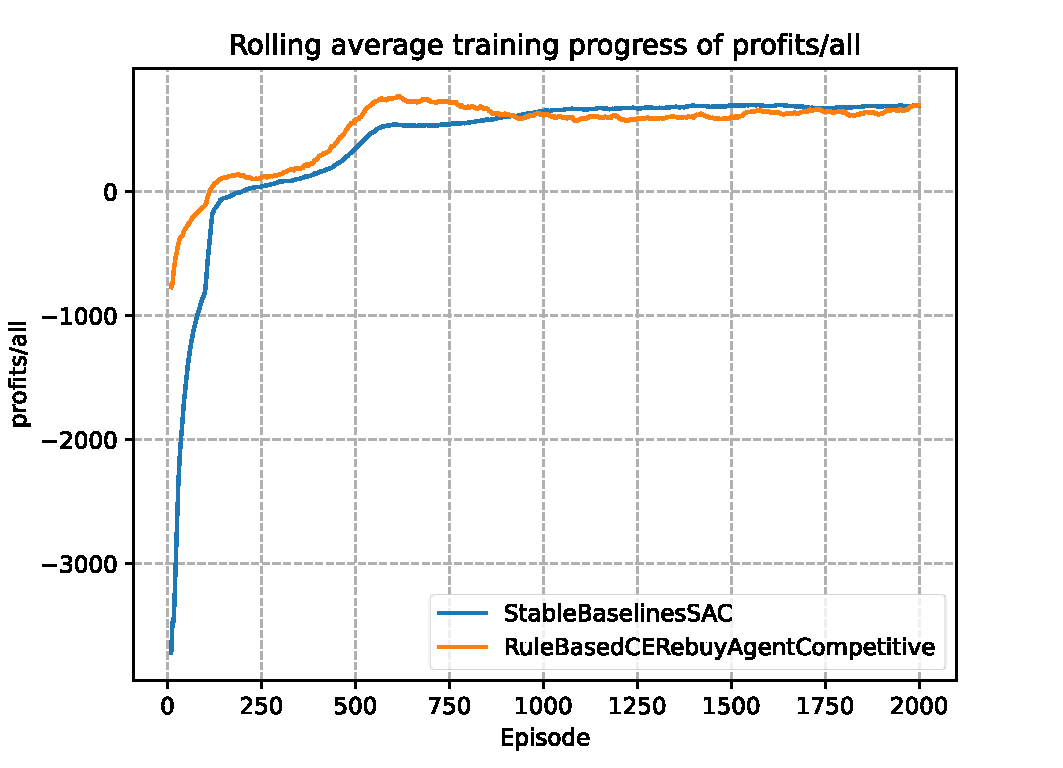
\includegraphics[width = \textwidth]{images/experiments/SACDuopoly/SACDuopolyProfitsMean1.pdf}\\
		\subcaption{SAC-Duopoly\_1, 2000 training episodes}\label{fig:SACDuopolyProfitsMean1}
	\end{subfigure}
	\begin{subfigure}{0.49\textwidth}
		\centering
		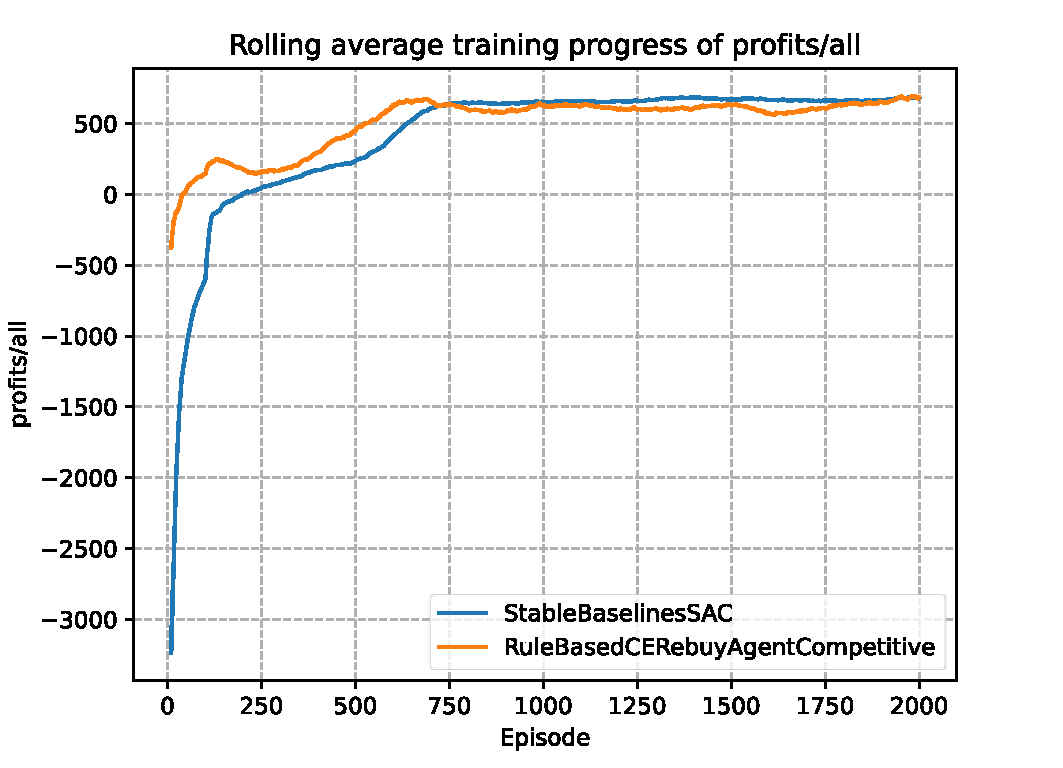
\includegraphics[width = \textwidth]{images/experiments/SACDuopoly/SACDuopolyProfitsMean2.pdf}\\
		\subcaption{SAC-Duopoly\_2, 2000 training episodes}\label{fig:SACDuopolyProfitsMean2}
	\end{subfigure}
	\begin{subfigure}{0.49\textwidth}
		\centering
		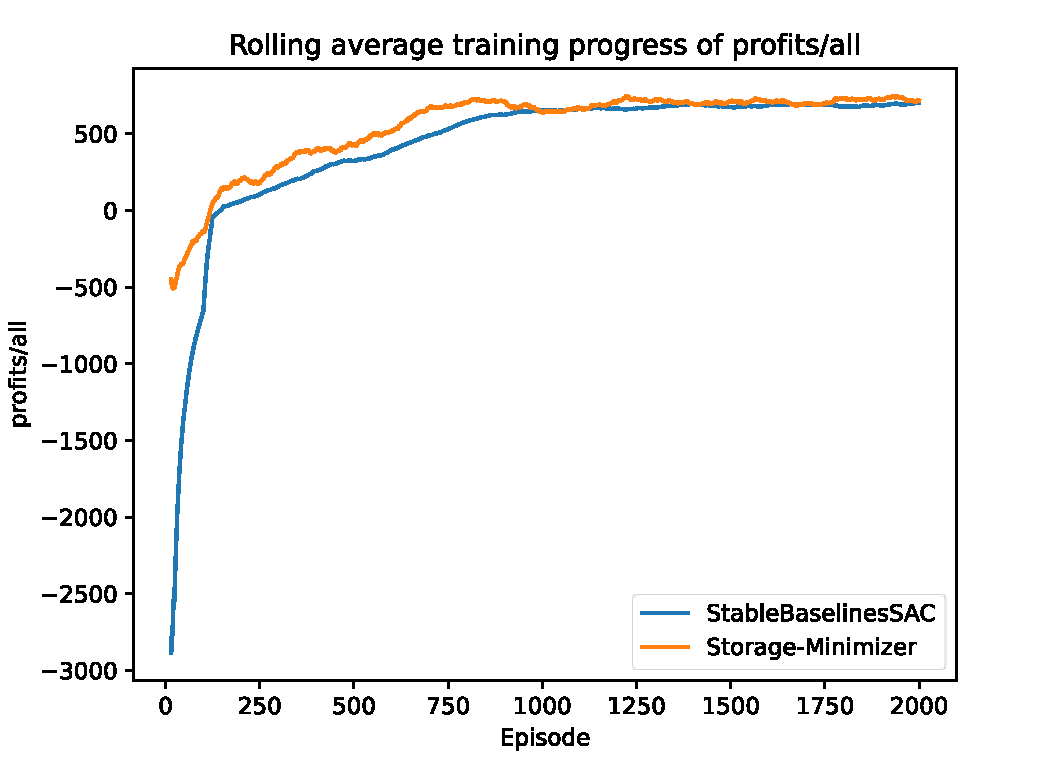
\includegraphics[width = \textwidth]{images/experiments/SACDuopoly/SACDuopolyProfitsMean3.pdf}\\
		\subcaption{SAC-Duopoly\_3, 2000 training episodes}\label{fig:SACDuopolyProfitsMean3}
	\end{subfigure}
	\begin{subfigure}{0.49\textwidth}
		\centering
		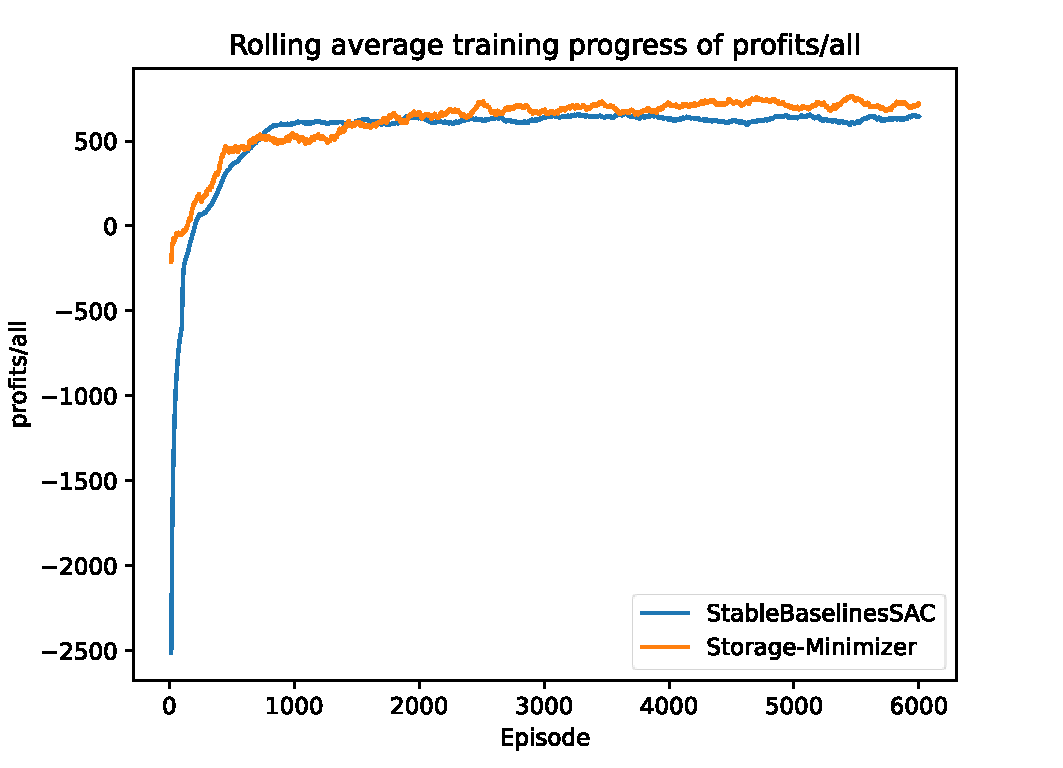
\includegraphics[width = \textwidth]{images/experiments/SACDuopoly/SACDuopolyProfitsMean4.pdf}\\
		\subcaption{SAC-Duopoly\_4, 6000 training episodes}\label{fig:SACDuopolyProfitsMean4}
	\end{subfigure}
	\caption{Profit per episode of four different training runs of an SAC-Agent on a Duopoly market.}\label{fig:SACDuopolyProfitsMean}
\end{figure}

This section will focus on the diagrams created by the Live-monitoring tool after training, which always runs an Agent-monitoring session as well, to immediately provide the user with many additional useful diagrams without the need to run the tool manually.

A commonly asked question when deciding on the quality of a Reinforcement-Learning agent is their \emph{stability}. If an algorithm is stable, the trained agent will produce similar results over multiple training sessions, on the condition that the parameters do not differ. Not only the rewards achieved at the end of the training will be very similar, but also the amount of episodes needed to reach certain thresholds. In the case of the SAC-Duopoly experiment, we ran the same configuration four times: The first three experiments were run using the exact same parameters, for the fourth experiment the amount of training episodes were tripled, meaning that the SAC-Agent had more time to alter its policy. \Cref{fig:SACDuopolyProfitsMean} shows the results of these four training sessions, created using the \nameref{subsec:LiveMonitoring} tool and visualizes the data collected during the training process. Although many other graphs are created (\Cref{tab:AllMetrics}), the visualization of the total profit of the agent is the most convenient to use when evaluating an agent's performance, as the total profit is the parameter which the agent is trying to optimize.

\Cref{fig:SACDuopolyProfitsMean} shows the stability of the SAC-Agent very well. The agent not only reached the break-even threshold of a reward of 0 after around 150 episodes in each of the four training runs, but no matter the total length of training (see the model in \Cref{fig:SACDuopolyProfitsDensity4}, which was trained three times as long as the others), the profit would always stabilize and stay at around 670. Had the monitoring tools shown that the agent performs worse than expected in some of the experiments, we could conclude that this particular algorithm is not fit for the type of work required by our market simulation.

We can also observe that the profits of the SAC-Agent and the Rule-Based agent (in the case of this experiment, a \emph{RuleBasedCERebuyAgentStorageMinimizer}) seem to be closely linked to each other in this particular scenario. In the beginning of each experiment, when the Reinforcement-Learning agent still knows very little about the market and makes great losses, the Rule-Based agent also has a hard time to perform well. However, as soon as the SAC-Agent starts to perform better, the Rule-Based agent is also able to increase its mean profits at around the same rate as the SAC-Agent. Even more interestingly, the agents not only increase their profits at the same rate, but also very quickly arrive at a point where they earn the same mean amount as the other.

This might lead one to believe that the two competitors' policies align closely with each other. To validate this claim, another type of diagram created by the Live-monitoring tool can be used: The density plots. These diagrams visualize probability densities for the various datasets recorded. While the diagrams shown in \Cref{fig:SACDuopolyProfitsMean} simply visualize data that was collected during the training run, density plots are created by running the Agent-monitoring tool, where the marketplace is simulated an additional time.\todo{This is explanatory, perhaps move it to the approaches chapter} This allows us to use the `intermediate' models we saved during the training run (see \nameref{subsec:LiveMonitoring}) to compare the Reinforcement-Learning Agent's policies at different points in time during the training.

\begin{figure}[t]
	\centering
	\begin{subfigure}{0.49\textwidth}
		\centering
		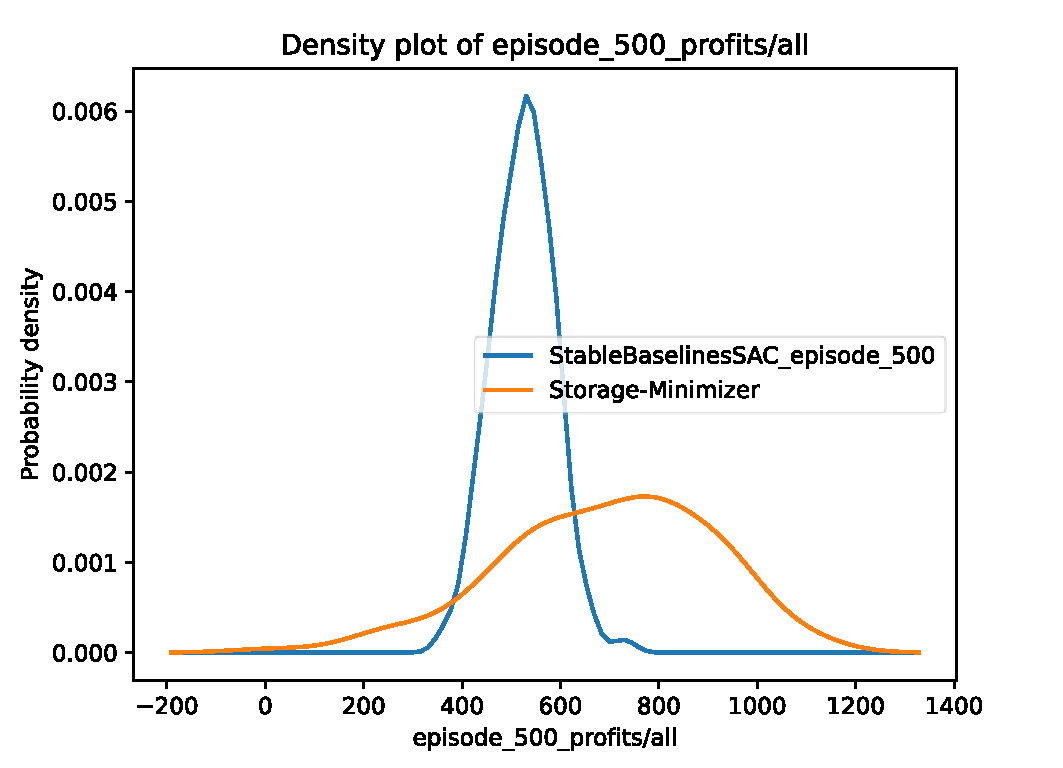
\includegraphics[width = \textwidth]{images/experiments/SACDuopoly/SACDuopolyProfitsDensity1.pdf}\\
		\subcaption{Model trained for 500 episodes}\label{fig:SACDuopolyProfitsDensity1}
	\end{subfigure}
	\begin{subfigure}{0.49\textwidth}
		\centering
		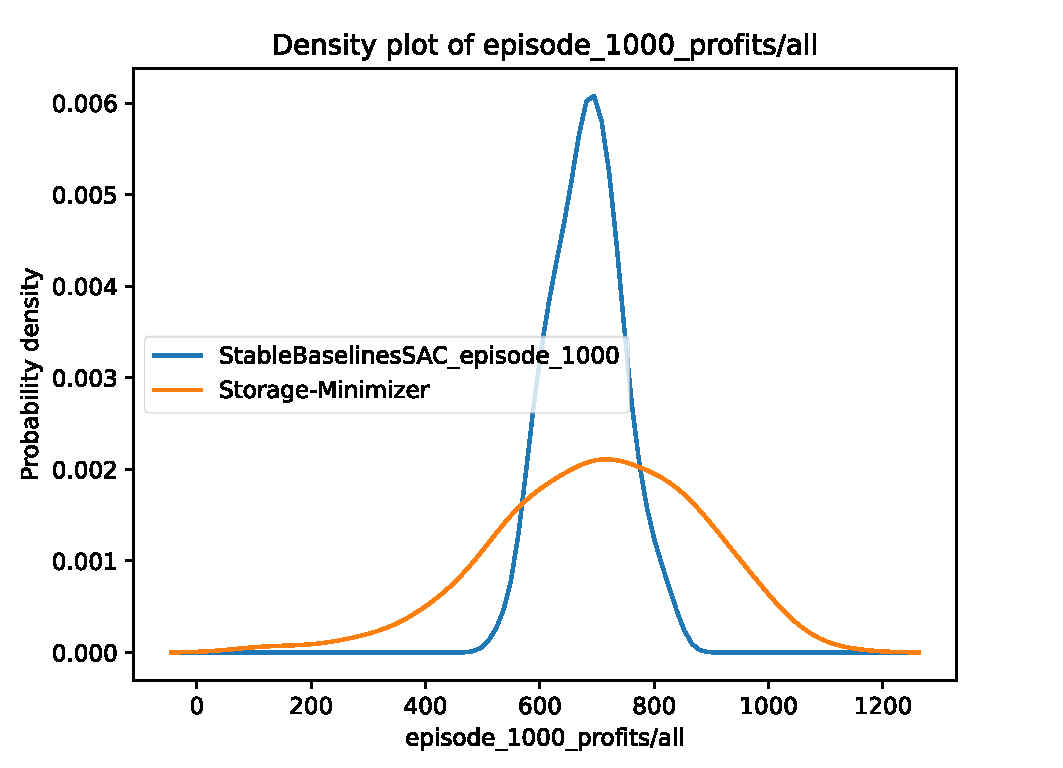
\includegraphics[width = \textwidth]{images/experiments/SACDuopoly/SACDuopolyProfitsDensity2.pdf}\\
		\subcaption{Model trained for 1000 episodes}\label{fig:SACDuopolyProfitsDensity2}
	\end{subfigure}
	\begin{subfigure}{0.49\textwidth}
		\centering
		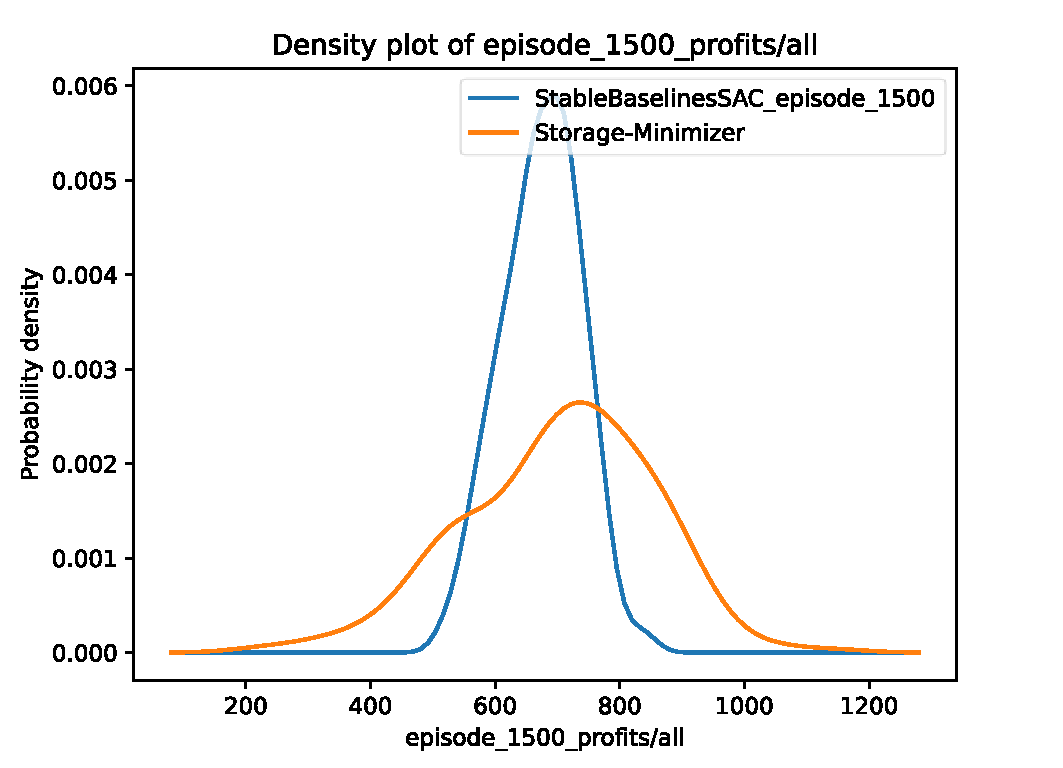
\includegraphics[width = \textwidth]{images/experiments/SACDuopoly/SACDuopolyProfitsDensity3.pdf}\\
		\subcaption{Model trained for 1500 episodes}\label{fig:SACDuopolyProfitsDensity3}
	\end{subfigure}
	\begin{subfigure}{0.49\textwidth}
		\centering
		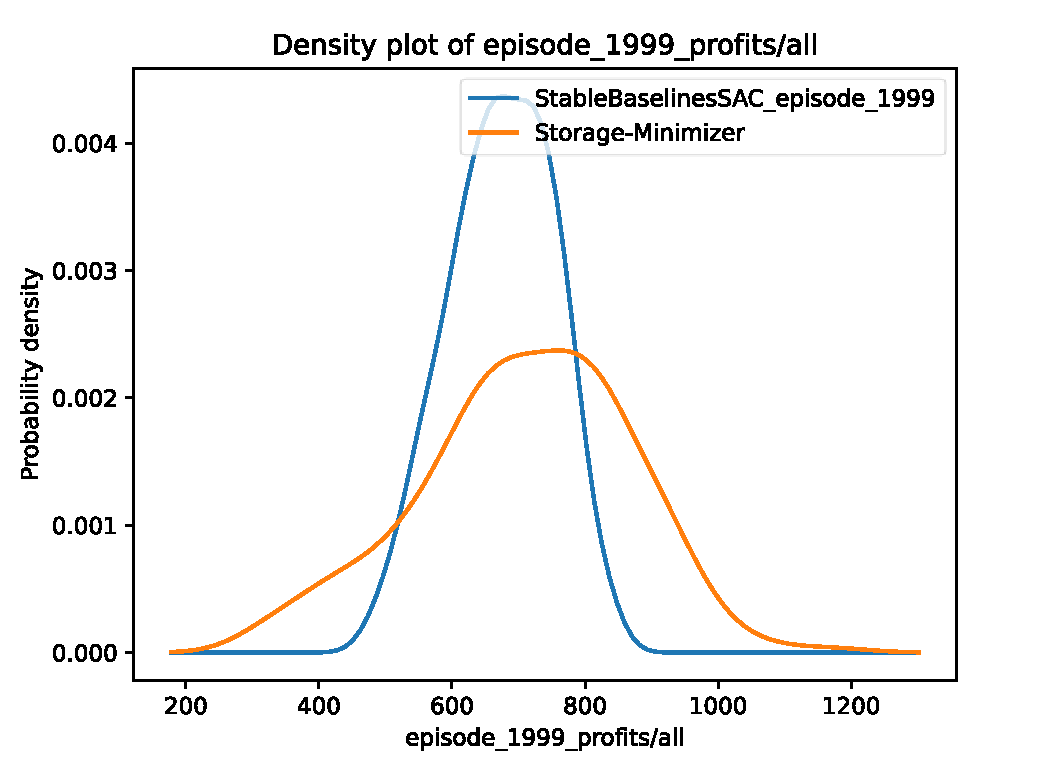
\includegraphics[width = \textwidth]{images/experiments/SACDuopoly/SACDuopolyProfitsDensity4.pdf}\\
		\subcaption{Model trained for 2000 episodes}\label{fig:SACDuopolyProfitsDensity4}
	\end{subfigure}
	\caption{Probability densities for achieving a certain profit for four different training stages of the SAC-Duopoly\_1 experiment.}\label{fig:SACDuopolyProfitsDensity}
\end{figure}

\Cref{fig:SACDuopolyProfitsDensity} shows the density plots of profit-per-episode for four different training stages of the SAC-Duopoly\_1 experiment. From this it can be concluded that the claim that the two competitors' policies align closely is incorrect: even though the mean reward within an episode is always very similar (\Cref{fig:SACDuopolyProfitsMean1}), the SAC-Agent achieves rewards which lie closer together, while the Rule-Based agent's rewards have more of a spread.

We can also observe that the models which were trained for longer are not necessarily better or even the same quality of the models with less experience. There is a significant improvement going from the model shown in \Cref{fig:SACDuopolyProfitsDensity1} to the one in \Cref{fig:SACDuopolyProfitsDensity2}, this shift in the probability density curve can be correlated with the maximum mean rewards the two models could achieve during the training: For the model trained on 500 episodes, this was around 450, for the other it was about 660 (\Cref{fig:SACDuopolyProfitsMean1}). Both of these values have respectively high probabilities of being reached during the second simulation after the training has concluded, i case of the model trained for 1000 episodes, this even coincides with the maximum in the density plot (\Cref{fig:SACDuopolyProfitsDensity2}). Going from the model trained on 1000 episodes to the next one, which was trained on 1500 episodes (\Cref{fig:SACDuopolyProfitsDensity3}), both the probability densities as well as the mean rewards stay very close to each other. From this we can conclude that training the SAC-Agent for more than 1000 episodes is very likely to not have a great effect on the maximum reward achievable by the algorithm. Going from the model trained on 1500 episodes to the last one, saved at the end of the training \Cref{fig:SACDuopolyProfitsDensity4}, we can however see a deterioration in performance: While the mean rewards hardly changed (\Cref{fig:SACDuopolyProfitsMean1}), the probability density curve got wider at its base, extending out further towards a reward of 400, and lowering the probability of achieving a reward of 700 from previously above 0.5\% to under 0.4\%. This means that the model which was trained for the longest time produces less predictable results than those trained less, which is a tame version of \emph{Catastrophic Forgetting}, as touched upon in \nameref{subsec:FutureLiveMonitoring}. The insights gained by our monitoring tools combined with the fact that we save `intermediate' models of the Reinforcement-Learning agent during training allows us to find the optimal trained model to use for further investigation and eventual deployment on the real market. In the case of the SAC-Duopoly\_1 experiment, the optimal model would be the one trained for 1000 episodes.

\subsubsection*{Further investigation}

Evaluating a model based on just the mean profits achieved by the monitored agents may not be enough for many users, which is why our Live-monitoring offers many other useful diagrams as well. In this section, we will take a look at a small selection of them. The graphs used will be from the SAC-Duopoly\_1 experiment.

Users may ask themselves how the profits achieved by the different vendors are split between the two available retail channels of new and refurbished products, how many products were bought back from customers or how much the vendors had to pay for storage of these used products. For all of these questions, the Live-monitoring (together with the Agent-monitoring) tool offers two types of diagrams: First, simple lineplots as shown in \Cref{fig:SACDuopolyProfitsMean} can be used, as well as scatterplots which visualize the exact data recorded during the episode, instead of the trends shown by the lineplots. \Cref{fig:SACDuopolyMixedGraphs} shows a number of different metrics such as the ones mentioned above, all of which are available as both linepots and scatterplots (\Cref{tab:AllMetrics}).

\begin{figure}[t]
	\centering
	\begin{subfigure}{0.49\textwidth}
		\centering
		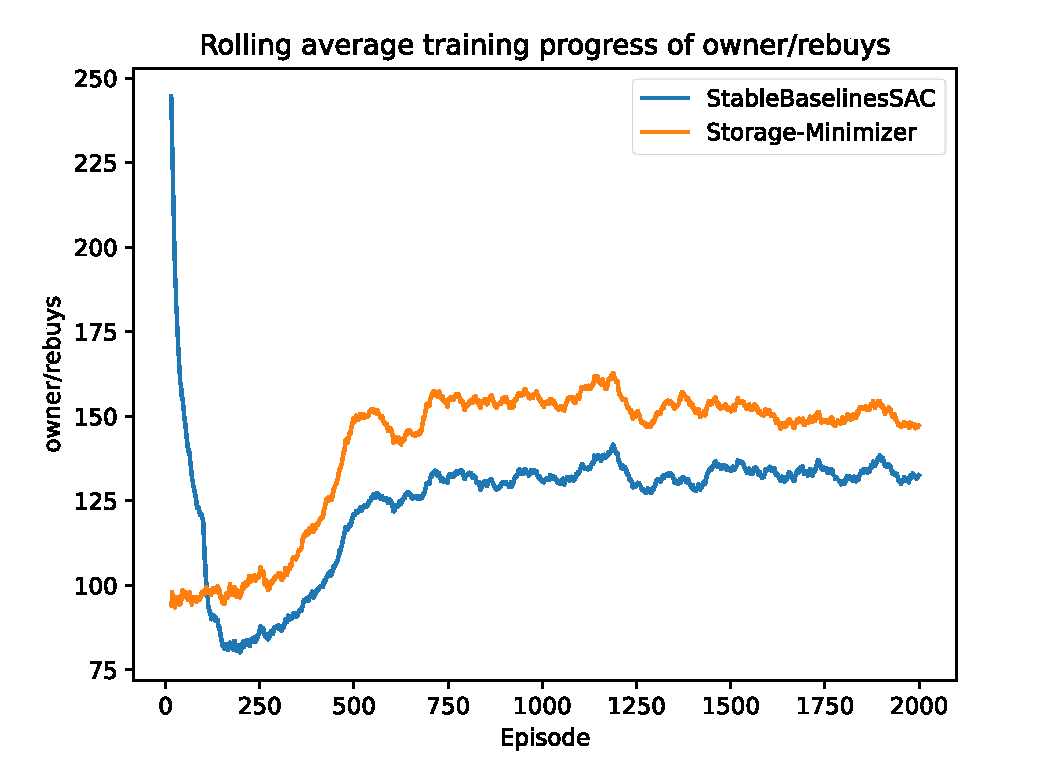
\includegraphics[width = \textwidth]{images/experiments/SACDuopoly/SACDuopolyMixedGraphs1.pdf}\\
		\subcaption{Amount of products sold back to vendors}\label{fig:SACDuopolyMixedGraphs1}
	\end{subfigure}
	\begin{subfigure}{0.49\textwidth}
		\centering
		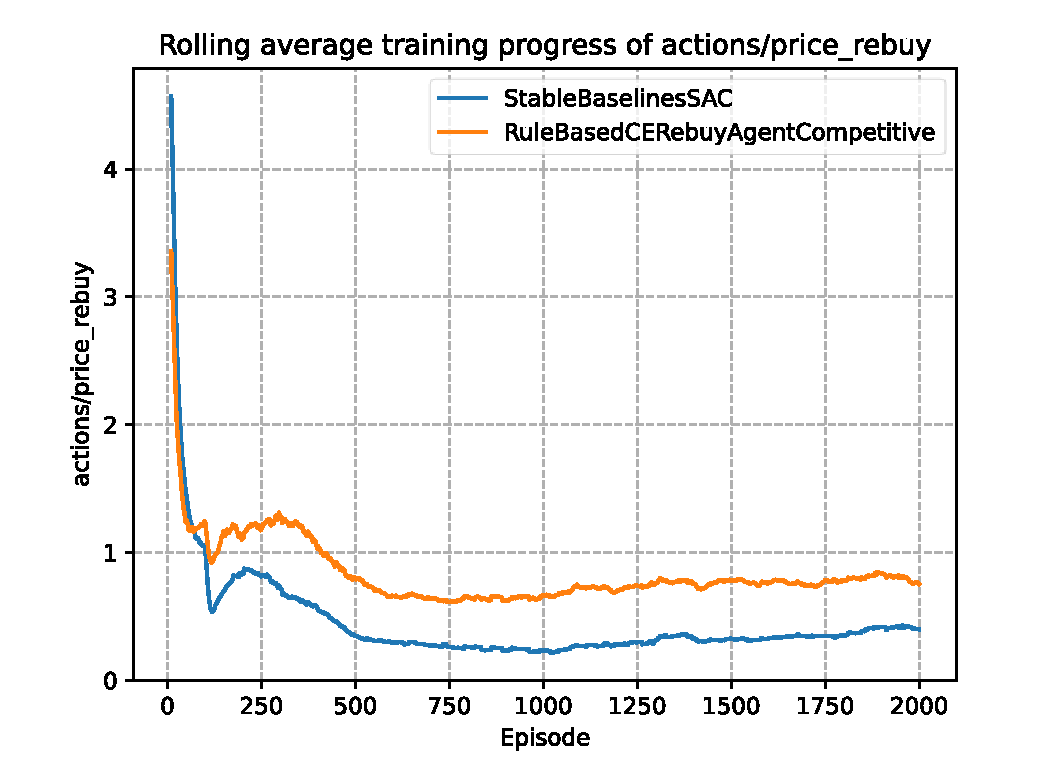
\includegraphics[width = \textwidth]{images/experiments/SACDuopoly/SACDuopolyMixedGraphs2.pdf}\\
		\subcaption{Storage costs for bought back products}\label{fig:SACDuopolyMixedGraphs2}
	\end{subfigure}
	\begin{subfigure}{0.49\textwidth}
		\centering
		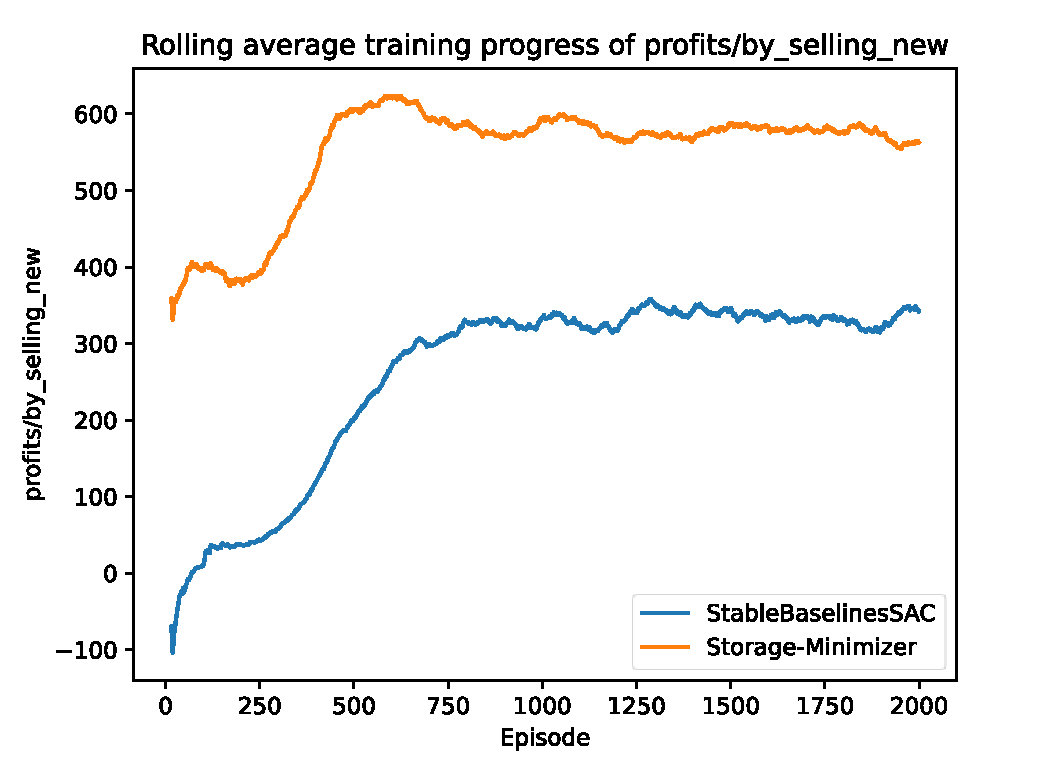
\includegraphics[width = \textwidth]{images/experiments/SACDuopoly/SACDuopolyMixedGraphs3.pdf}\\
		\subcaption{Profit from selling new products}\label{fig:SACDuopolyMixedGraphs3}
	\end{subfigure}
	\begin{subfigure}{0.49\textwidth}
		\centering
		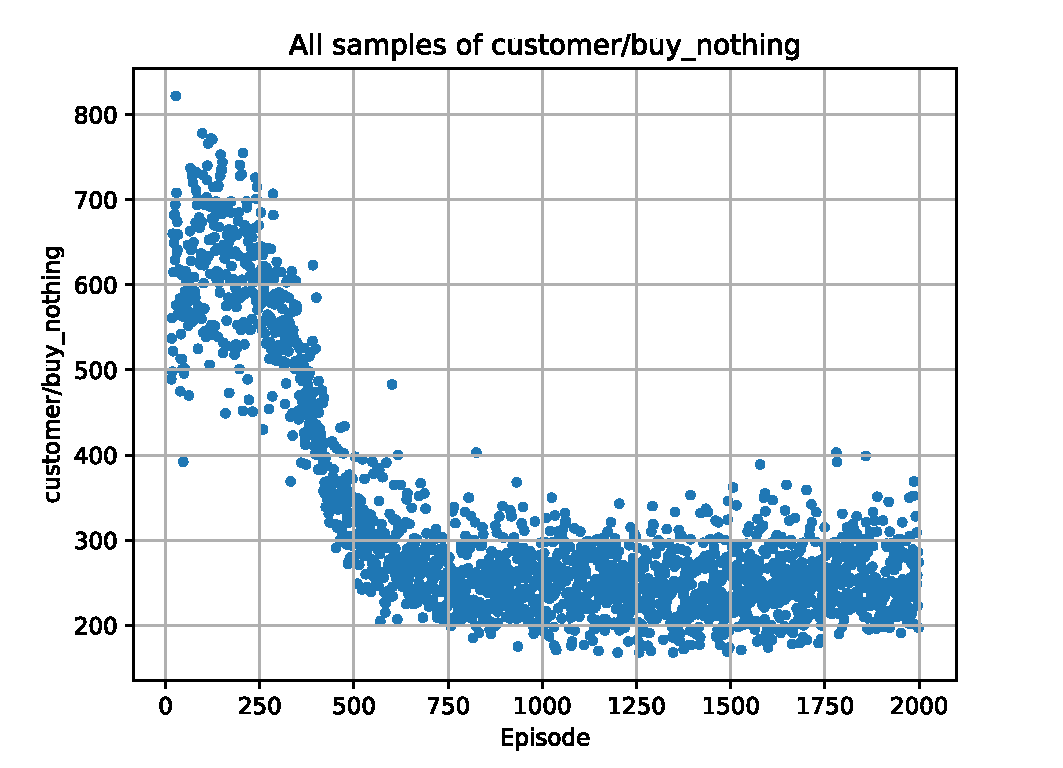
\includegraphics[width = \textwidth]{images/experiments/SACDuopoly/SACDuopolyMixedGraphs4.pdf}\\
		\subcaption{Customers that bought nothing}\label{fig:SACDuopolyMixedGraphs4}
	\end{subfigure}
	\caption{Diagrams visualizing various datapoints collected during training of the SAC-Duopoly\_1 experiment.}\label{fig:SACDuopolyMixedGraphs}
\end{figure}

Many connections can be made when evaluating different diagrams side-by-side, such as the observation of the initially high storage costs of the SAC-Agent in \Cref{fig:SACDuopolyMixedGraphs2} being caused by a very high number of products that were bought back from customers (\Cref{fig:SACDuopolyMixedGraphs1}), which is in turn a cause of high rebuy prices set by the Reinforcement-Learning Agent, making it more likely that customers sell back their products. High storage and rebuy costs will have then caused a policy change to set lower rebuy prices, thereby de-incentivizing customers to sell back as many products as they used to and lowering the agent's storage costs.

The next pair of diagrams tells us two things: First, the vendors' initially low profits from selling new products as shown in \Cref{fig:SACDuopolyMixedGraphs3}, or in the bigger picture, low profits overall (\Cref{fig:SACDuopolyProfitsMean1}) were not caused by the vendors setting prices that are too low, but rather too high. This is confirmed by an initially very high number of customers which chose to not buy any of the products offered by the vendors (\Cref{fig:SACDuopolyMixedGraphs4}). Additionally, when comparing the total profits of the two vendors with the profits gained from selling only new products (\Cref{fig:SACDuopolyProfitsMean1} and \Cref{fig:SACDuopolyMixedGraphs3}), we can come to the conclusion that the SAC-Agent must have learned to prioritize selling refurbished products over new ones and keeping storage costs low, since we know that overall profits for the two vendors are about the same in the later parts of the training, but the SAC-Agent sells a lot less new products than its Rule-Based counterpart.

If the Agent-monitoring is run after a training session (with a number of intermediate models), it also creates violinplots for all of the collected metrics (\Cref{tab:AllMetrics}). A selection of such diagrams can be found in \Cref{fig:SACDuopolyViolinPlots}, showing the respective total profits (\Cref{fig:SACDuopolyViolinPlots1}) and storage costs (\Cref{fig:SACDuopolyViolinPlots2}) for each intermediate model of the trained SAC-Agent. As explained in \nameref{subsec:AgentMonitoring}, these plots visualize the probability distributions as shown in \Cref{fig:SACDuopolyProfitsDensity} in a more condensed way, providing additional data such as actual maximum, minimum and median values as well. The biggest upside of the Violinplots is however that they are able to show the distributions for all intermediate models in one diagram, which allows for even better comparisons. Looking at \Cref{fig:SACDuopolyViolinPlots1} we can immediately see the difference in the spread of total profits achieved between the models trained for 1500 and 2000 episodes respectively, for which we previously needed to consult and compare two different diagrams (\Cref{fig:SACDuopolyProfitsDensity3} and \Cref{fig:SACDuopolyProfitsDensity4}). Similarly, \Cref{fig:SACDuopolyViolinPlots2} is able to tell us something else we did not know before: the longer a model was trained for, the more likely it is that it will induce high storage costs, a trend which was not necessarily visible in \Cref{fig:SACDuopolyMixedGraphs2}.

Violinplots do however not replace the need for density plots, as both have an equally useful way of displaying data. While the violinplots show rough distributions plotting against the real numbers on the y-axis, the density plots show the concrete probability values for each possible datapoint.

\begin{figure}[t]
	\centering
	\begin{subfigure}{0.49\textwidth}
		\centering
		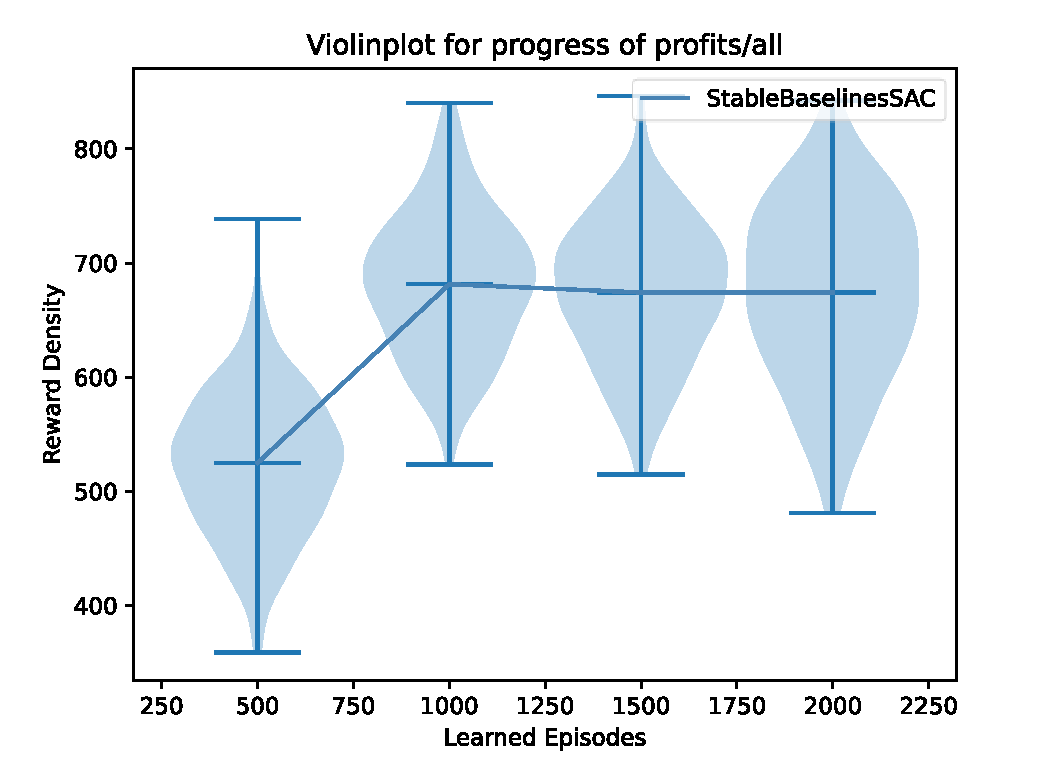
\includegraphics[width = \textwidth]{images/experiments/SACDuopoly/SACDuopolyProfitsAllViolin.pdf}\\
		\subcaption{Total profits for all intermediate models}\label{fig:SACDuopolyViolinPlots1}
	\end{subfigure}
	\begin{subfigure}{0.49\textwidth}
		\centering
		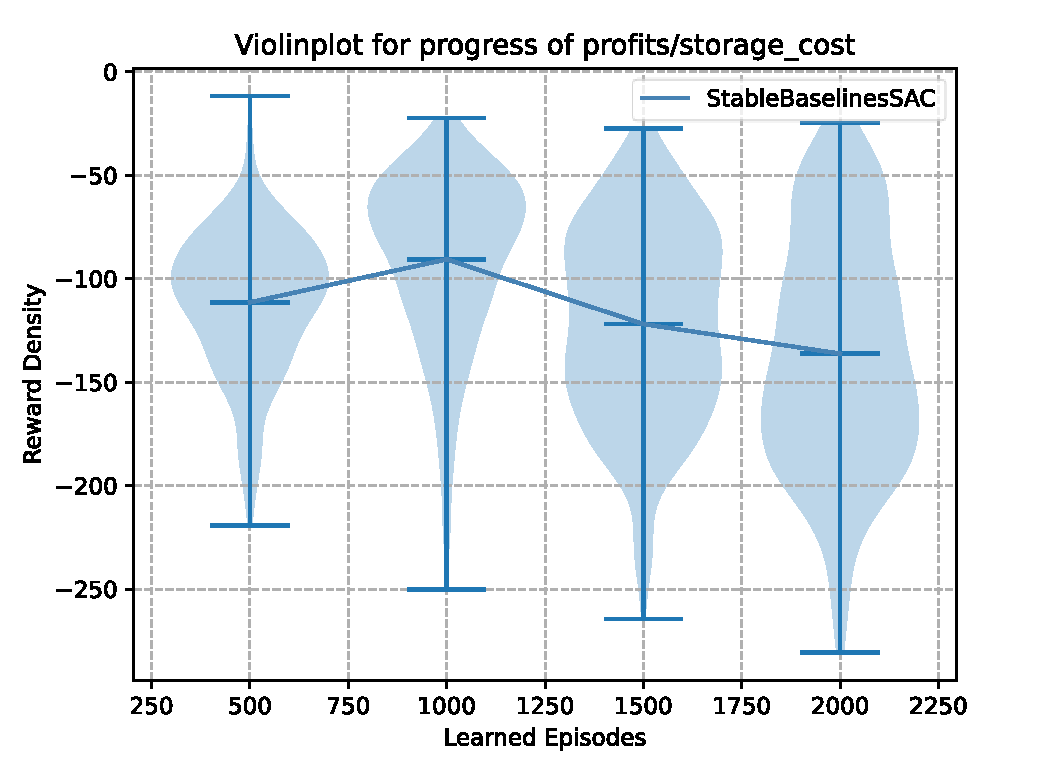
\includegraphics[width = \textwidth]{images/experiments/SACDuopoly/SACDuopolyStorageCostsViolin.pdf}\\
		\subcaption{Storage costs for all intermediate models}\label{fig:SACDuopolyViolinPlots2}
	\end{subfigure}
	\caption{Violinplots showing a selection of collected data when running Agent-monitoring after training.}\label{fig:SACDuopolyViolinPlots}
\end{figure}

\subsection*{Exampleprinter}

Run an exampleprinter, insert one frame of svg. Mention that it is normally animated. Talk about why this offers more or new info than the Live/Agent-monitoring.

\subsection*{Policyanalyzer}

Run two different Policyanalyzer-runs: Once with only one feature, once with two features. Show how the info can be used to inform on the agent's quality. Maybe show one instance where it is not very useful.

\subsection*{Why not run Agent-monitoring? If not, why is it separate from Live-monitoring}

We do not run it, as it is already run with the Live-monitoring. So after training, we do not need to do it again. It still exists, as you may want to monitor the trained models independentl of each other using different parameters, or to monitor only Rule-Based agents.

\section*{Less useful diagrams}\label{sec:UselessDiagrams}

This section is meant to highlight a number of diagrams which are not very useful, such as the `Statistics diagrams'. The reason for this can be twofold: Either the data shown in the diagram is not inertly useful, or the graph provides duplicated or confusing information.

\section*{Some sort of conclusion here}

% \section*{Which graphs are how useful?}
% \section*{What limitations are there?}
% \section*{What can we do in the future to improve the graphs or the workflow?}

%%%%%%%%%%%%%%%%%%%%%%%%%%%%%%%%%
%% End of adding your content. %%
%%%%%%%%%%%%%%%%%%%%%%%%%%%%%%%%%


% Add the following chapters not to the current ›part‹ but one level above instead.
\makeatletter
\def\toclevel@chapter{-1}
\def\toclevel@section{0}
\makeatother

% \chapter{Conclusions \& Outlook}
% \label{ch:Conclusions}

\begin{jointwork}
	In this final chapter, we will look back at our framework and give an outlook on how different parts of it, especially the monitoring tools, could be improved in the future. This will be followed by a short summary of the learnings from this thesis.
\end{jointwork}

\section{Modelling a realistic \emph{recommerce} marketplace}\label{sec:DivergingFromRealMarket}

We do not claim in any way that our simulation framework is exhaustive or complete. This section will focus on ways in which different parts of it could or should be improved in the future, to model a more realistic marketplace.

% There are a number of parameters influencing market dynamics, small and great, which have not been modelled due to time constraints or their unpredictability in their effect on the market state or customer decisions. Seasonality of demand, customer retention, loyalty through branding and unforeseen effects on market dynamics such as global events (for example, the Covid-19 pandemic) are just some of the places where our market simulation diverges from the real market, following its inability to model these circumstances. However, all of these factors are either very rare in nature (global, unforeseen events), only applicable to a subset of markets (brand loyalty) or can initially be discarded as their effect on market dynamics is predictable, making them a lower priority than other parameters (seasonality).

% The factors mentioned above all have an impact on both Linear and Circular markets, but there are also a number of parameters that are specific to Circular or even recommerce markets in particular.
In the modern recommerce market, more and more consumers make their initial purchasing decisions with the product's eventual resale value already in mind~\cite{ShoppingResaleValue}. Additionally, a great number of different motivations for choosing second-hand or refurbished products over traditional new ones can be identified. An exemplary study conducted in 2008~\cite{SecondHandMotives} classified such motivations into 15 different categories (see \Cref{tab:SecondHandMotives}), all of which could be used to add dimensions to customer behaviour in our simulation framework, thereby making the whole simulation more realistic.

Our current limited customer behaviour results in the fact that our framework can not be used out-of-the-box for any kind of market. However, great care was taken during the development process to build each part of the simulation in a modular way, so that new functionality can easily be integrated into it. Marketplaces, customers and vendors (rule-based as well as those using Reinforcement learning) have all been implemented as classes disconnected from each other, so that new variants of each can easily be added to the pool of available options to be used in experiments. The same goes for our monitoring tools, all of which have been built to work with any (valid) combination of input parameters. For reference, all of the classes shown in \Cref{fig:OverviewDiagram} can be extended or replaced with ease. Please also refer to \cite{LeoThesis} for more information on the modularity of our framework.

The lack of realism on certain areas of the framework does not directly impact the way that our monitoring tools work or can be used. It must however be noted that the interpretation of results must always be based on the knowledge of these limitations.

\section{Improving our monitoring tools}\label{sec:ImprovingMonitoringTools}

While the previous section focussed on ways in which our simulation framework could be extended to be more realistic, this section will instead focus on ways in which our various monitoring tools could be improved. While all of the tools currently at our disposal are able to do what is expected of them and they each have their own strengths, there are still a number of ways that they could be enhanced.

%% This has now been added and is also shown in the AllMetrics diagram already.
% Before going into detail about the different tools, there is one enhancement which concerns all of our tools. As some tools are older than others and not only the tools itself but also the way we simulate our market has changed over time during development, not all tools record the same data. For example, the Exampleprinter records all prices set by vendors, but does not show a breakdown of profits between the different retail channels. On the other hand, the Agent-monitoring does offer such a breakdown, but does not record the vendors' actions and thereby prices. This can lead to confusion, as users may expect a certain type of diagram to be created when using one tool or the other. So an important, though perhaps time-intensive, enhancement would be to \textbf{unify the data that is being recorded across all monitoring tools}.

\subsection{Live-monitoring}\label{subsec:FutureLiveMonitoring}

The current downside of the Live-monitoring tool is that users need to wait until the training session has concluded before diagrams are created and the Agent-monitoring tool is run on the saved intermediate models.
% Currently, the Live-monitoring tool works by first taking and visualising all the data collected during a training run and then running the Agent-monitoring tool on the saved intermediate models. The biggest downside to this is that users need to wait until the training session has finished before the Live-monitoring is run, meaning that a lot of potential information is lost.
For example, imagine a scenario where a training session was initialised to run for 10,000 episodes, saving intermediate models each 1,000 episodes. In the end, when the Live-monitoring tool is run, the user may find that the best model was the one saved after 3,000 episodes, meaning that a lot of time was wasted training an additional 7,000 episodes. The possibility of this happening may at first seem counterintuitive, but is a common phenomenon when training RL agents, known as \emph{Catastrophic Forgetting} (see also \cite{CatastrophicForgetting}). By improving the Live-monitoring tool with an option to \textbf{run the Agent-monitoring whenever an intermediate model is saved}, the user would be able to recognise such trends much faster and terminate the experiment at the right time. This feature could be further enhanced with a smart built-in option that \textbf{terminates the experiment for the user if a downward trend in performance is detected}. Specific thresholds for these terminations should also optionally be \textbf{set by the user}. For this, the data created during the Live-monitoring tool would need to be saved in a machine-readable form - graphs and diagrams are not useful here.

\subsection{Agent-monitoring}\label{subsec:FutureAgentMonitoring}

This brings us to improvements that could be made to the Agent-monitoring tool. At the moment, a lot of data is recorded when simulating the marketplace, but only graphs and diagrams are created as a result of the simulation. By \textbf{giving users the option to have data saved a \texttt{.csv} files}, users would be enabled to use the results of the simulation in other ways more easily, even for monitoring and evaluation tools completely disconnected from our own framework and the tools we provide. Reproducibility is also a major concern when it comes to evaluating simulation results, as was already mentioned in \cbfref{ch:RelatedWork} and is discussed in many papers such as~\cite{DRLThatMatters} and~\cite{ReproducibilityRL}. In our simulation framework, with the start of a new episode the market state is always shuffled randomly, to allow Reinforcement learning algorithms to properly explore the environment. This is however creating the problem of creating simulations which are currently impossible to reproduce, which could be solved by \textbf{introducing a seed-based system for shuffling market states and sharing this seed with the user}. When running a different simulation with the same seed, assuming that the marketplace type and environment stay the same, users can recreate the same random market states that are set at the start of an episode. This allows for even better and in-depth comparisons of different vendors, past a single run of the Agent-monitoring tool. This seed-system could also be applied to the training workflow.

\subsection{Exampleprinter}\label{subsec:FutureExampleprinter}

The Exampleprinter is a great tool for quickly monitoring and evaluating a certain market setup. However, only for one specific combination of marketplace type and market environment, a Duopoly scenario of a Circular Economy with rebuy prices, the animated overview diagram is created. \textbf{Building templates and adding diagram support for more scenarios} should therefore be a priority when enhancing the Exampleprinter. Additionally, the \textbf{market-seed feature} introduced in \bfref{subsec:FutureAgentMonitoring} should also be implemented for the Exampleprinter, to allow users to run a simulation multiple times to monitor possible discrepancies in agent behaviour and find outliers in the data. This could be further enhanced by adding a configuration option that allows for \textbf{more than one episode to be simulated at a time}.

As a combined enhancement for both the Agent-monitoring and the Exampleprinter, the \textbf{Exampleprinter could be integrated into the Agent-monitoring}, while still being its own tool, the same as the Agent-monitoring is integrated into the Live-monitoring.

\subsection{Policyanalyser}\label{subsec:FuturePolicyAnalyser}

The biggest and most important improvement to the Policyanalyser does not concern its concrete features, but the way users interact with it. Currently, all of the other monitoring tools are either integrated into some part of the workflow (e.g. the Live-monitoring), or can easily be started using simple commands, see \cbfref{ch:OurWorkflow}. This is however not the case for the Policyanalyser, which must be started by going into the code itself, which is less than ideal from a user-perspective. So, \textbf{integrating the Policyanalyser into the workflow}, both by \textbf{creating a user-facing interface} for it and by \textbf{adding configuration options to start it after a training session} are features that should be a priority when continuing work on the framework. Users are also able to use the Policyanalyser to analyse a large number and combination of features, so \textbf{curating a list of useful feature combinations to be analysed} would aid many users when using this tool.

\section{Summary}

Using the market simulation framework that was built within the scope of the bachelor's project, users can simulate complex recommerce market situations. Thanks to the modular nature of the framework, different components, such as customer behaviour, can be updated, exchanged or added upon to create a configuration that fits the individual use case. The goal of such simulations is to enable users to implement, test and evaluate various dynamic pricing methods. While classically rule-based pricing methods play a big part in the framework, the majority of implemented and tested pricing methods are those based on Reinforcement learning algorithms, a machine learning technology. The goal of using such algorithms is to automate and optimise the dynamic pricing problem in the recommerce market environment. By using our framework, users are provided with a large number of tools to monitor, compare and evaluate any combination of pricing methods, enabling them to find the right fit for their needs. The provided tools work on many different levels, from those simulating large amounts of episodes, allowing for an analysis of potential macro-economic implications following specific approaches, to those that work on th smallest possible scale, testing an agent's pricing policy against every possible combination of market states and competitor actions. This allows for a thorough investigation of different strengths and weaknesses of the monitored pricing agents, a necessary prerequisite before being able to employ them in the real market and giving them power over actual pricing decisions.


% Following are the files and commands for the bibliography and the author’s publications.
\pagestyle{plain}

\renewcommand*{\bibfont}{\small}
\printbibheading
\addcontentsline{toc}{chapter}{Bibliography}
\printbibliography[heading = none]

\addchap{Appendix}
\section{Tables}

\begin{table}[ht]
	\begin{tabular}{p{0.35\textwidth} p{0.65\textwidth}}
		\toprule
		Consumer Characteristic                 & Description                                                                                                            \\\midrule
		Perfectionistic, High-Quality Conscious & Consumer searches carefully and \newline systematically for the very best quality in products                          \\
		Brand Conscious, `Price = Quality'      & Consumer is oriented towards buying the more expensive, well-known brands                                              \\
		Novelty and Fashion Conscious           & Consumers who like new and innovative products and gain excitement from seeking out new things                         \\
		Recreational and Shopping Conscious     & Consumer finds shopping a pleasant activity and enjoys shopping just for the fun of it                                 \\
		Price Conscious/ Value for the Money    & Consumer with a particularly high consciousness of sale prices and lower prices in general                             \\
		Impulsive/ Careless                     & Consumer who buys on the spur of the moment and appears unconcerned about how much he/she spends                       \\
		Confused by Overchoice                  & Consumer perceiving too many brands and stores from which to choose and experiences information overload in the market \\
		Habitual/ Brand Loyal                   & Consumer who repetitively chooses the same favorite brands and stores                                                  \\\bottomrule
	\end{tabular}\\
	\caption{Consumer Shopping Styles, from~\cite{ShoppingStyles}, including information from~\cite{ShoppingStyles2}.}\label{tab:shoppingStyles}
\end{table}

\begin{table}[!]
	\begin{tabular}{p{1\textwidth}}
		\toprule
		I - Economic dimensions                                                              \\\midrule
		1. ECO1 - Buying cheaper, spending less (anxiety expressed in regard to expenditure) \\
		2. ECO2 - Paying fair prices                                                         \\
		3. ECO3 - Allocative role of price (what is obtained for a particular budget)        \\
		4. ECO4 - Bargain hunting                                                            \\
		\toprule
		II - Dimensions relating to the nature of the offering                               \\\midrule
		5. OFF1 - Originality                                                                \\
		6. OFF2 - Nostalgia                                                                  \\
		7. OFF3 - Congruence                                                                 \\
		8. OFF4 - Self-expression                                                            \\
		\toprule
		III - Dimensions relating to the recreational aspects of second-hand channels        \\\midrule
		9. CIR1 - Social contact                                                             \\
		10. CIR2 - Stimulation                                                               \\
		11. CIR3 - Treasure hunting                                                          \\
		\toprule
		IV - Power dimensions                                                                \\\midrule
		12. PUIS1 - Smart shopping                                                           \\
		13. PUIS2 - Power over the seller                                                    \\
		\toprule
		V - 14. ETH - Ethical and ecological dimension                                       \\
		\toprule
		VI - 15 ANT-OST - Anti-ostentation dimension                                         \\
		\bottomrule
	\end{tabular}\\
	\caption{15 areas of motivation toward second-hand shopping, from~\cite{SecondHandMotives} (descriptions omitted).}\label{tab:SecondHandMotives}
\end{table}

\begin{table}[!]
	\begin{tabular}{|cr|p{2.2mm}|p{2.2mm}|p{2.2mm}|p{2.2mm}|p{2.2mm}|p{2.2mm}|p{2.2mm}|p{2.2mm}|p{2.2mm}|p{2.2mm}|p{2.2mm}|p{2.2mm}|p{2.2mm}|p{2.2mm}|p{2.2mm}|p{2.2mm}|}
		\hline
		\multicolumn{2}{|l|}{}                                       & \rotatebox{90}{state/in\_circulation} & \rotatebox{90}{state/in\_storage} & \rotatebox{90}{action/price\_new} & \rotatebox{90}{action/price\_refurbished} & \rotatebox{90}{action/rebuy\_price} & \rotatebox{90}{owner/throw\_away} & \rotatebox{90}{owner\_rebuys} & \rotatebox{90}{customer/purchase\_new} & \rotatebox{90}{customer/purchase\_refurbished\space} & \rotatebox{90}{customer/buy\_nothing} & \rotatebox{90}{profit/rebuy\_cost} & \rotatebox{90}{profit/storage\_cost} & \rotatebox{90}{profit/by\_new} & \rotatebox{90}{profit/by\_refurbished} & \rotatebox{90}{profit/all} & \rotatebox{90}{profit/reward}     \\ \hline
		\multicolumn{2}{|r|}{Exampleprinter}                         & X                                     &                                   & X                                 & X                                         & X                                   & X                                 & X                             & X                                      & X                                                    &                                       &                                    &                                      &                                &                                        & X                          &                                   \\ \hline
		\multicolumn{2}{|r|}{TensorBoard}                            & X                                     & X                                 & X                                 & X                                         & X                                   & X                                 & X                             & X                                      & X                                                    & X                                     & X                                  & X                                    & X                              & X                                      & X                          & X                                 \\ \hline
		\multicolumn{1}{|c|}{\multirow{2}{*}{\rotatebox{90}{Live}}}  & Scatter                               & X                                 & X                                 & X                                         & X                                   & X                                 & X                             & X                                      & X                                                    & X                                     & X                                  & X                                    & X                              & X                                      & X                          & X                             &   \\ \cline{2-18}
		\multicolumn{1}{|r|}{}                                       & Line                                  & X                                 & X                                 & X                                         & X                                   & X                                 & X                             & X                                      & X                                                    & X                                     & X                                  & X                                    & X                              & X                                      & X                          & X                             &   \\ \hline
		\multicolumn{1}{|c|}{\multirow{3}{*}{\rotatebox{90}{Agent}}} & Density                               & X                                 & X                                 & X                                         & X                                   & X                                 & X                             & X                                      & X                                                    & X                                     & X                                  & X                                    & X                              & X                                      & X                          & X                             & X \\ \cline{2-18}
		\multicolumn{1}{|r|}{}                                       & Violin                                & X                                 & X                                 & X                                         & X                                   & X                                 & X                             & X                                      & X                                                    & X                                     & X                                  & X                                    & X                              & X                                      & X                          & X                             & X \\ \cline{2-18}
		\multicolumn{1}{|r|}{}                                       & Line                                  & X                                 & X                                 & X                                         & X                                   & X                                 & X                             & X                                      & X                                                    & X                                     & X                                  & X                                    & X                              & X                                      & X                          & X                             & X \\ \hline
	\end{tabular}\\
	\caption{All metrics recorded during the simulation and which monitoring tools visualize them.}\label{tab:AllMetrics}
\end{table}

\newpage
\section{Rule-based agents - Policies}\label{sec:AppendixPolicies}

\begin{figure}[ht]
	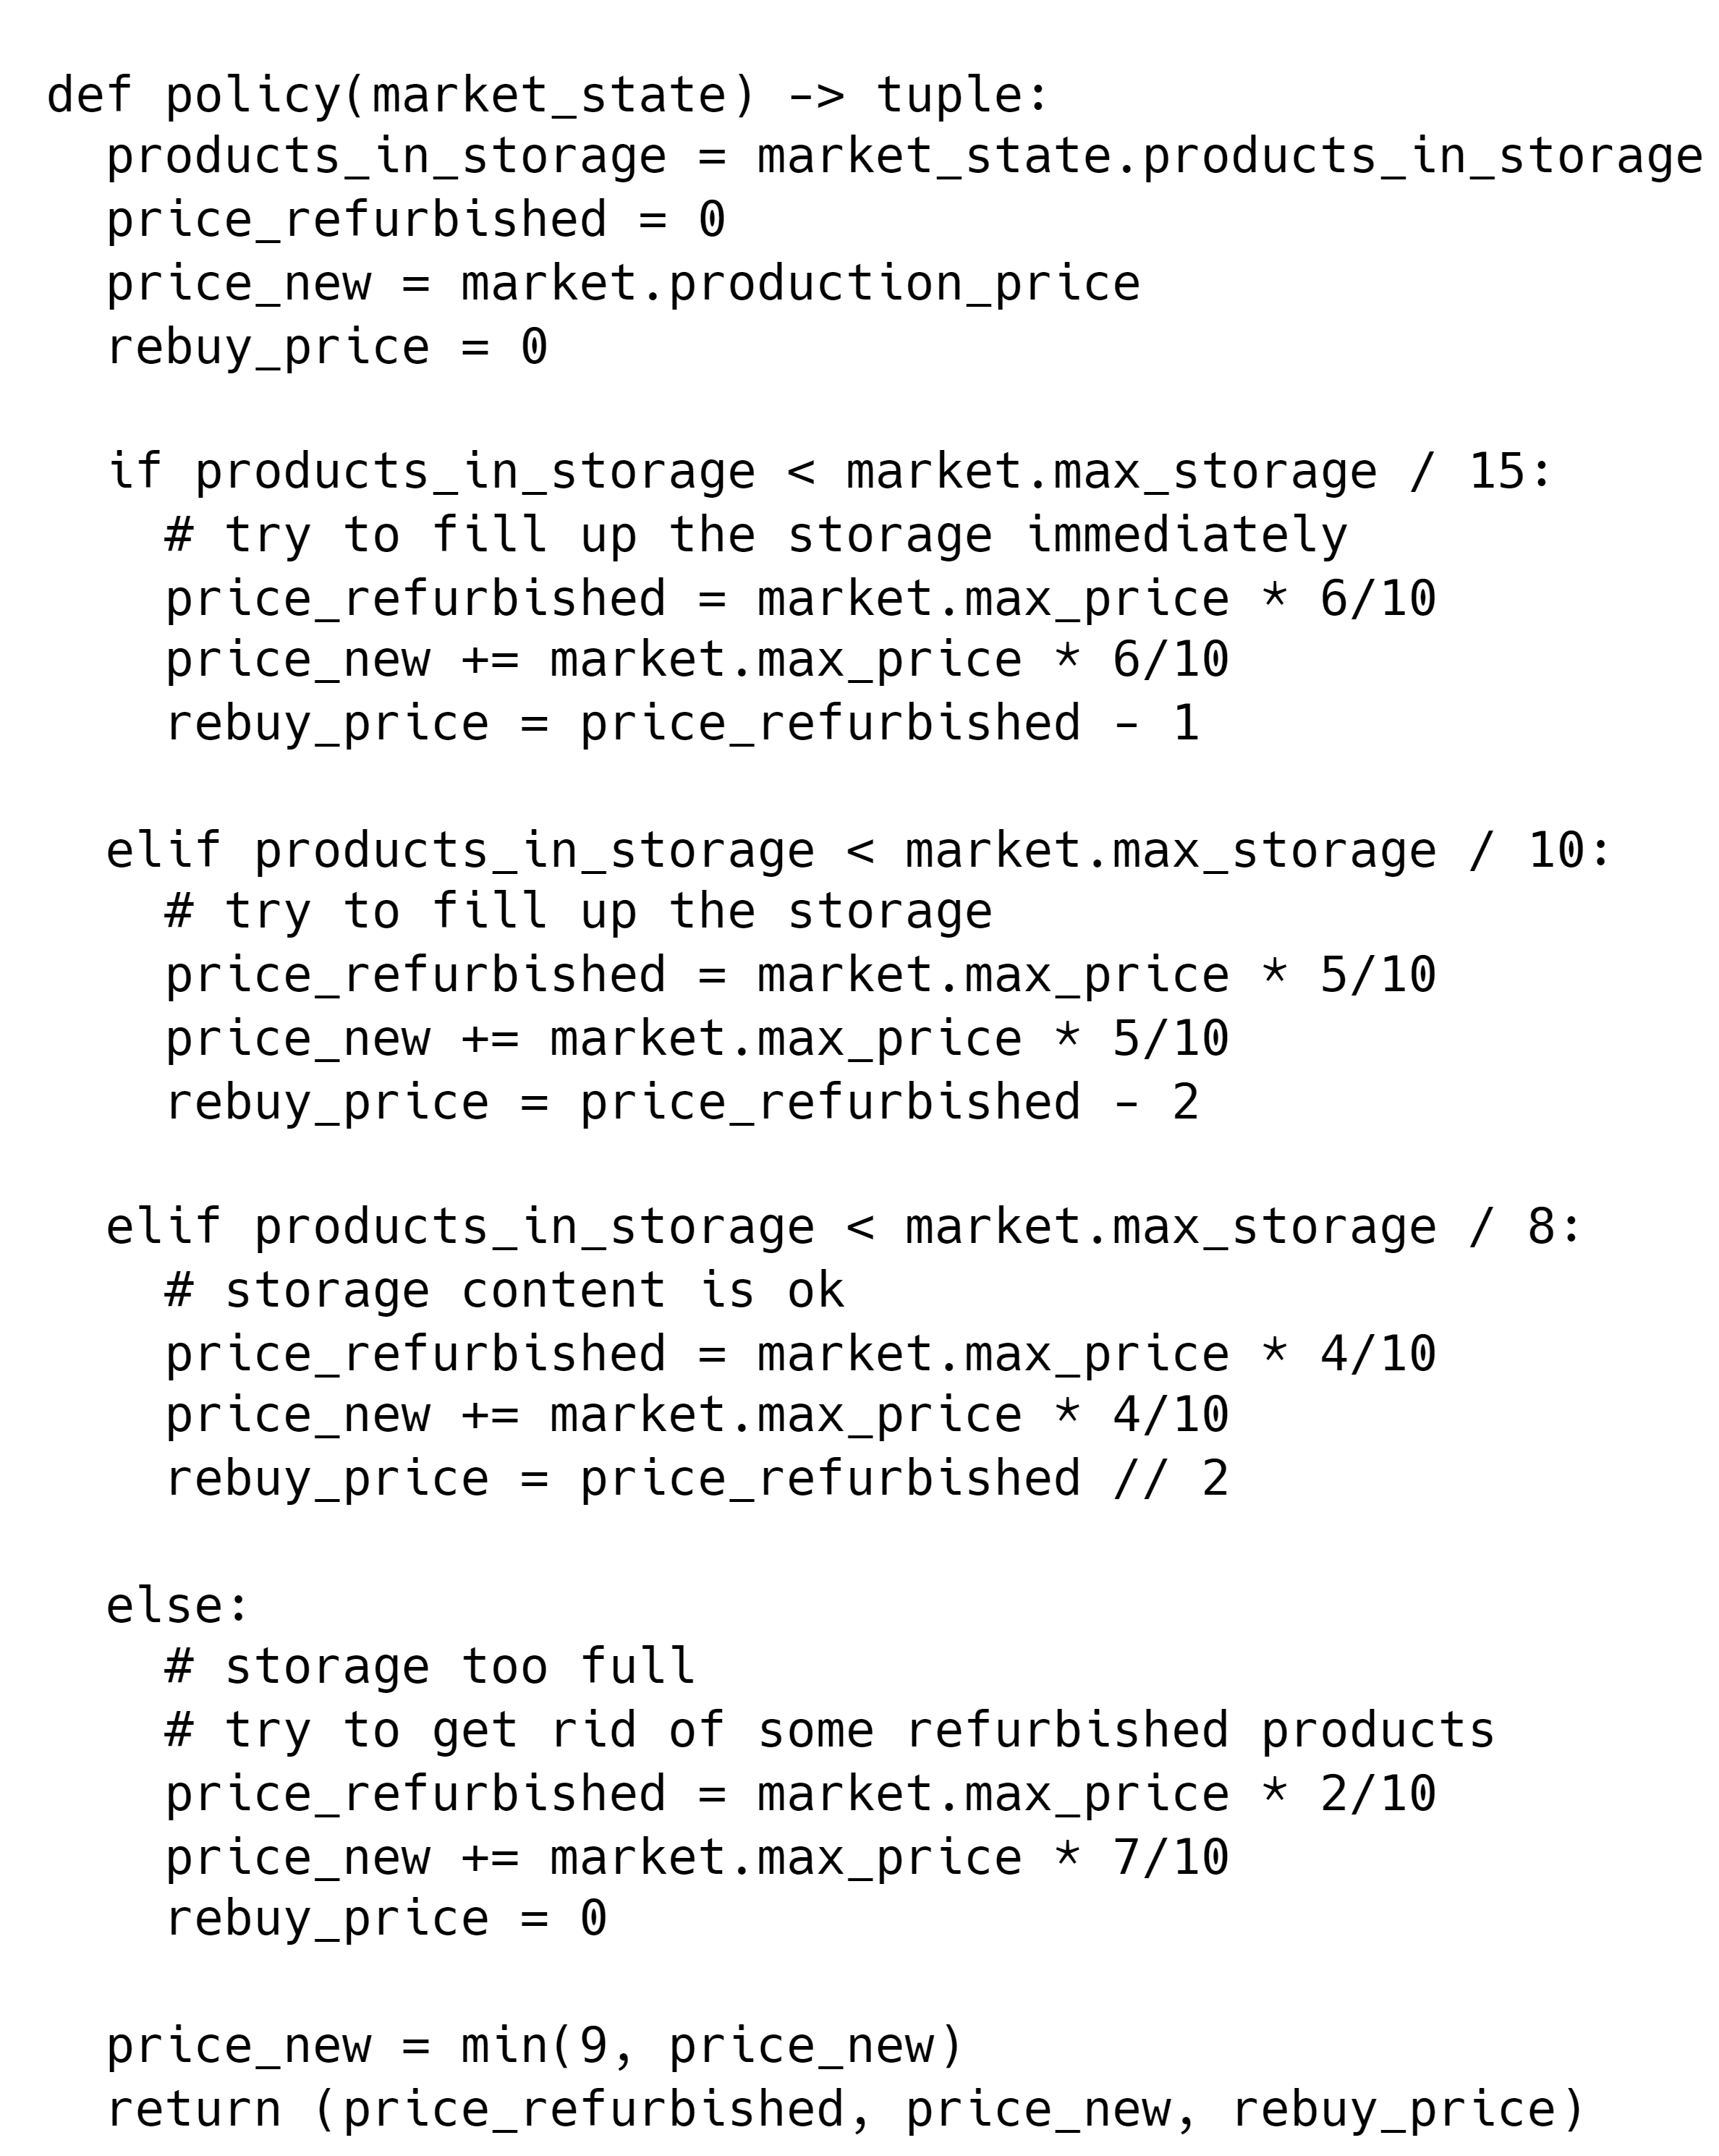
\includegraphics[width = \textwidth]{images/policies/RuleBasedCERebuyAgentPolicy.png}\\
	\caption{Policy implementation of the \emph{RuleBasedCERebuyAgent}, simplified for readability.}\label{fig:PolicyRuleBasedCERebuy}
\end{figure}

\begin{figure}[ht]
	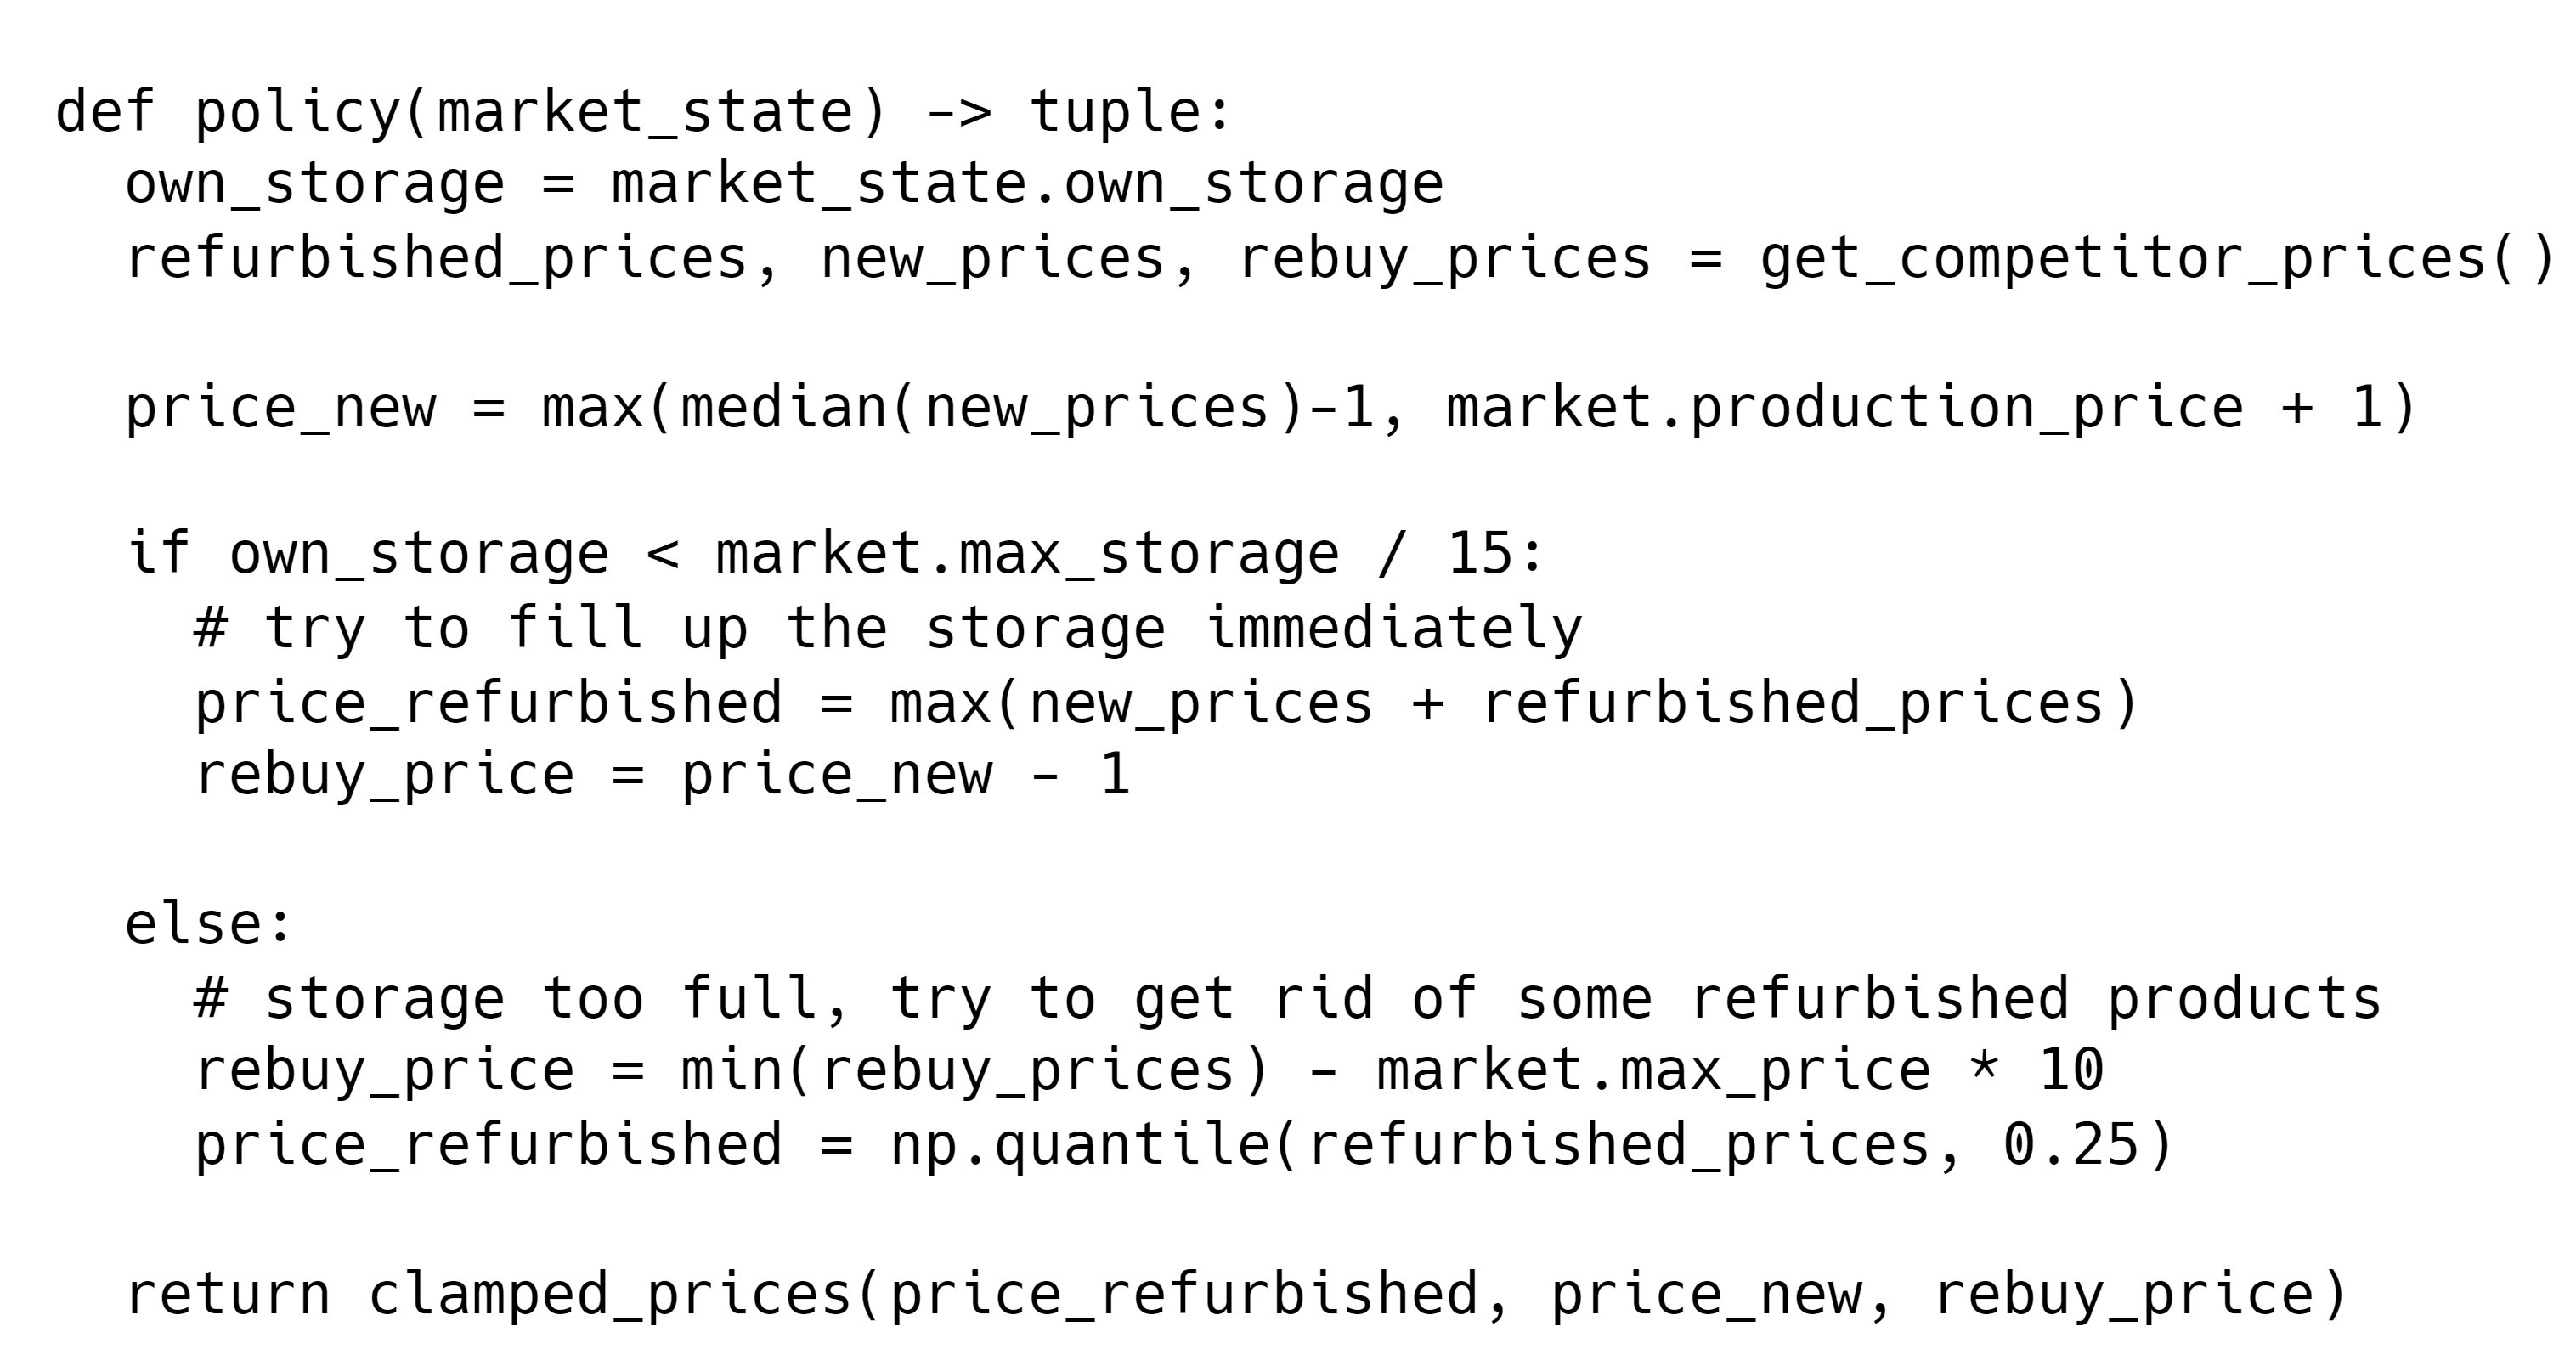
\includegraphics[width = \textwidth]{images/policies/RuleBasedCERebuyAgentStorageMinimizerPolicy.png}\\
	\caption{Policy implementation of the \emph{RuleBasedCERebuyAgentStorageMinimizer}, simplified for readability.}\label{fig:PolicyRuleBasedStorageMinimizer}
\end{figure}

\begin{figure}[ht]
	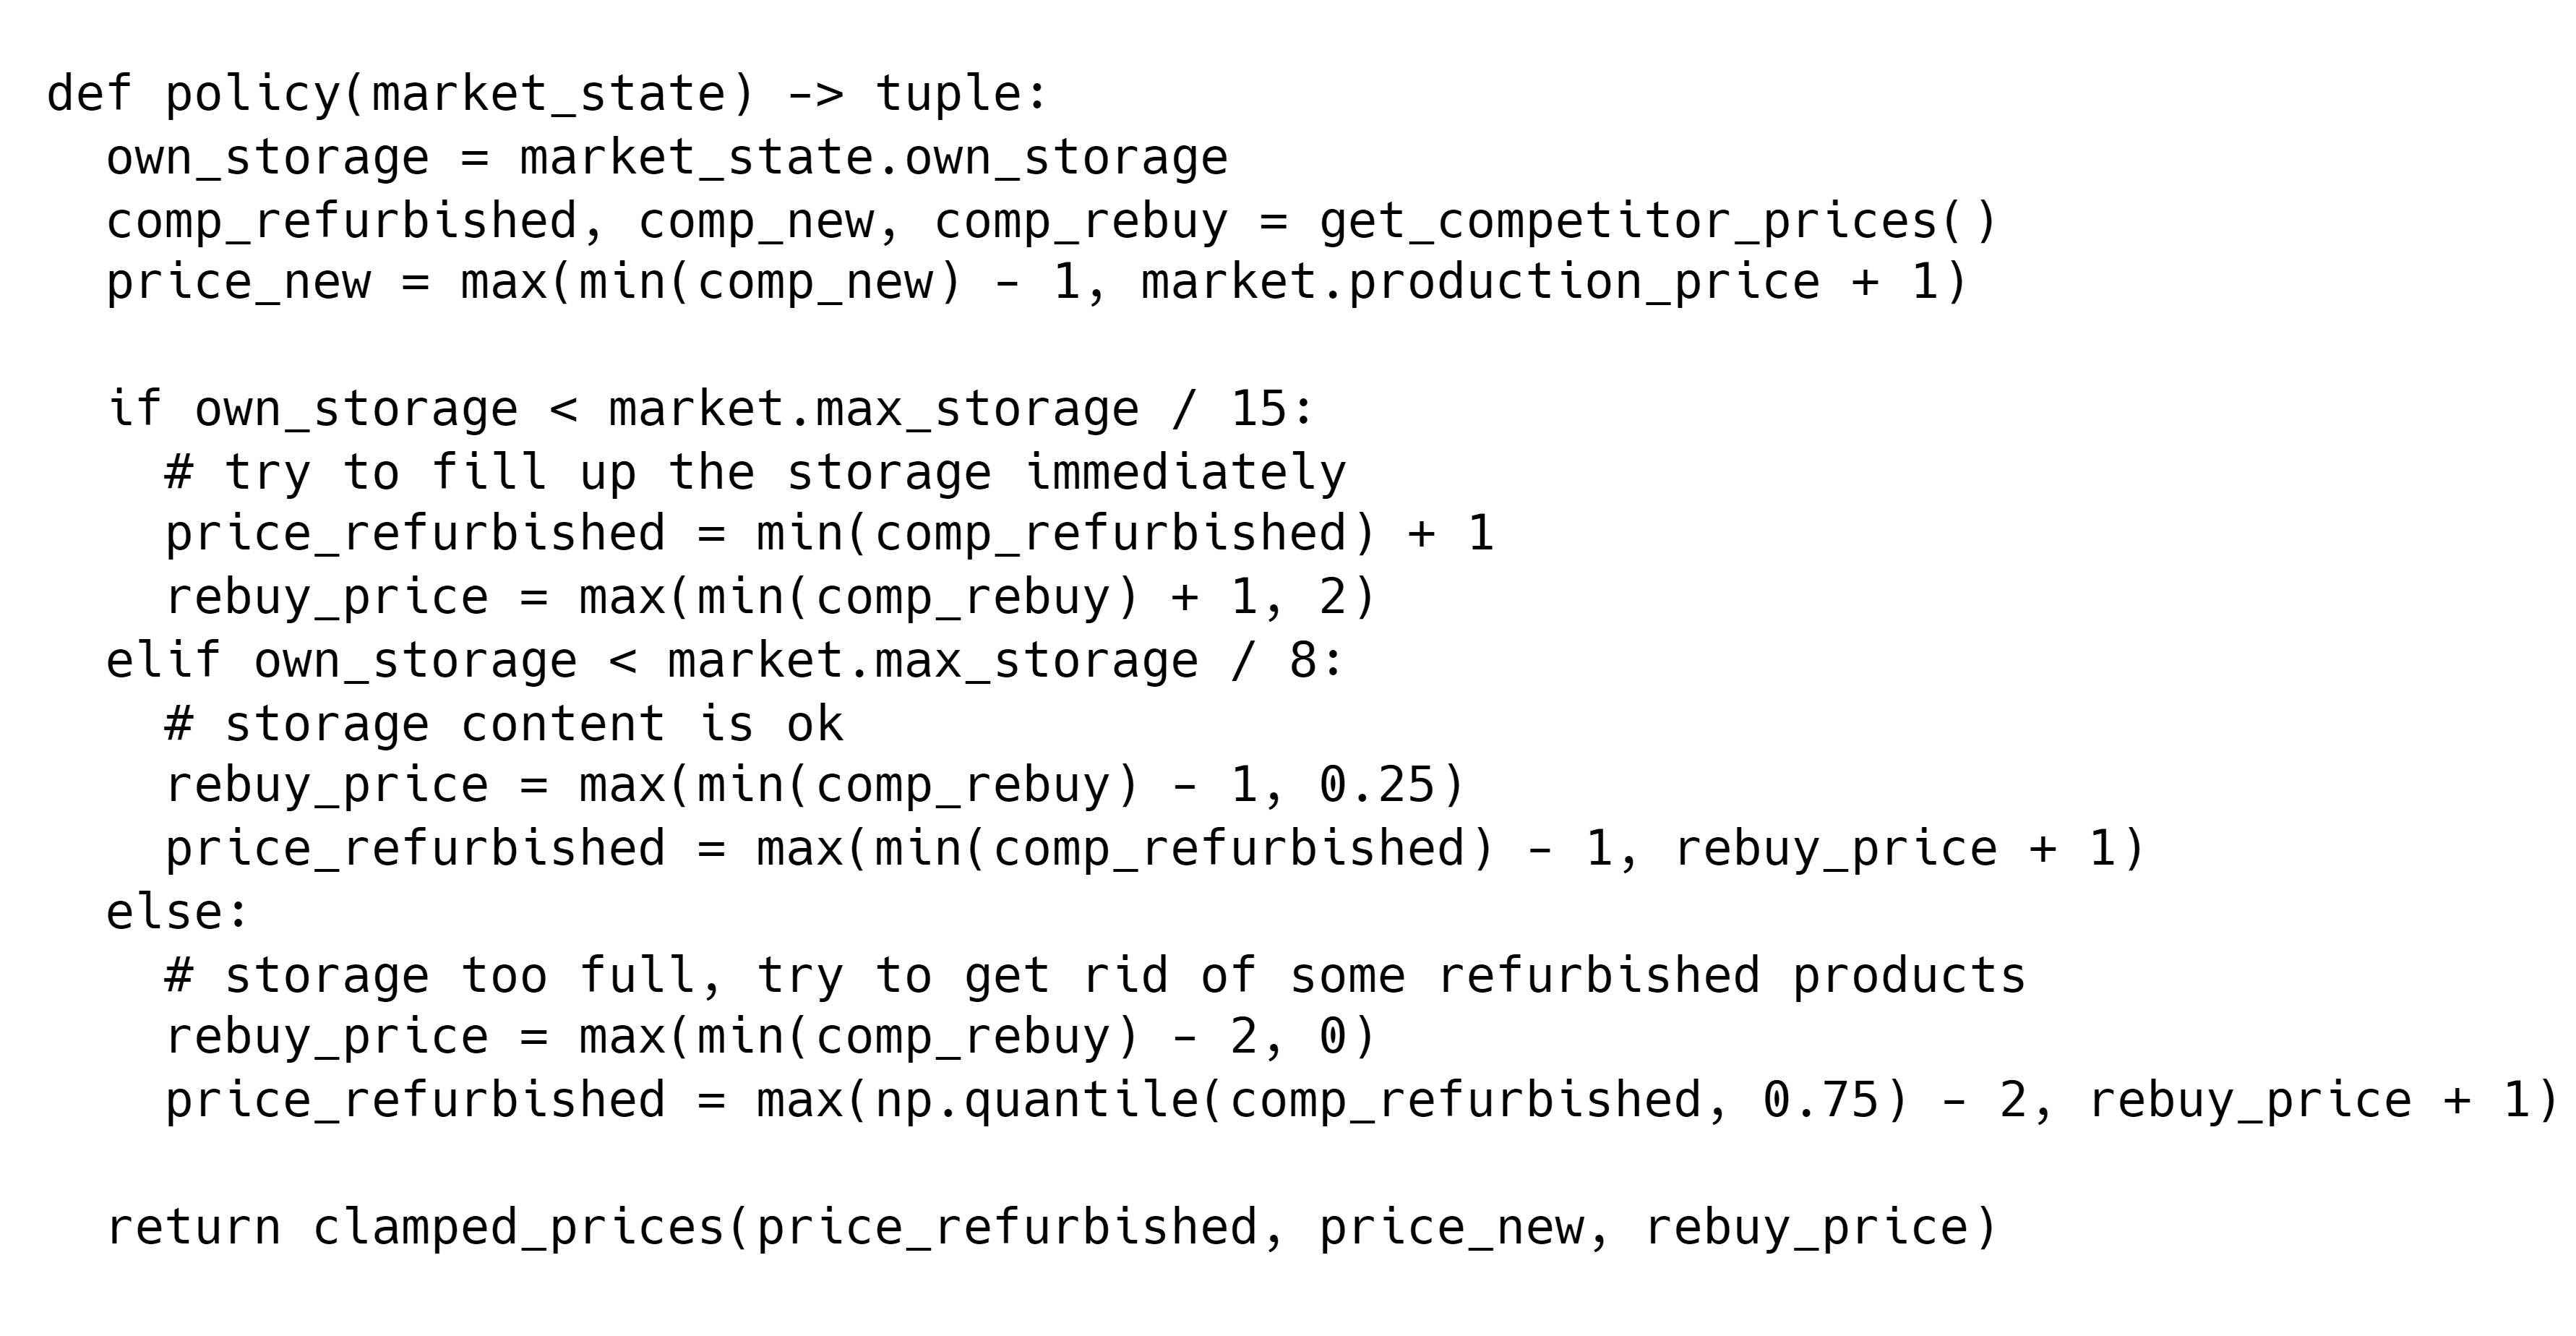
\includegraphics[width = \textwidth]{images/policies/RuleBasedCERebuyAgentCompetitivePolicy.png}\\
	\caption{Policy implementation of the \emph{RuleBasedCERebuyAgentCompetitive}, simplified for readability.}\label{fig:PolicyRuleBasedCompetitive}
\end{figure}

\clearpage
\section{SAC-Duopoly experiment - Configuration files}\label{sec:AppendixConfigFiles}

\begin{figure}[ht]
	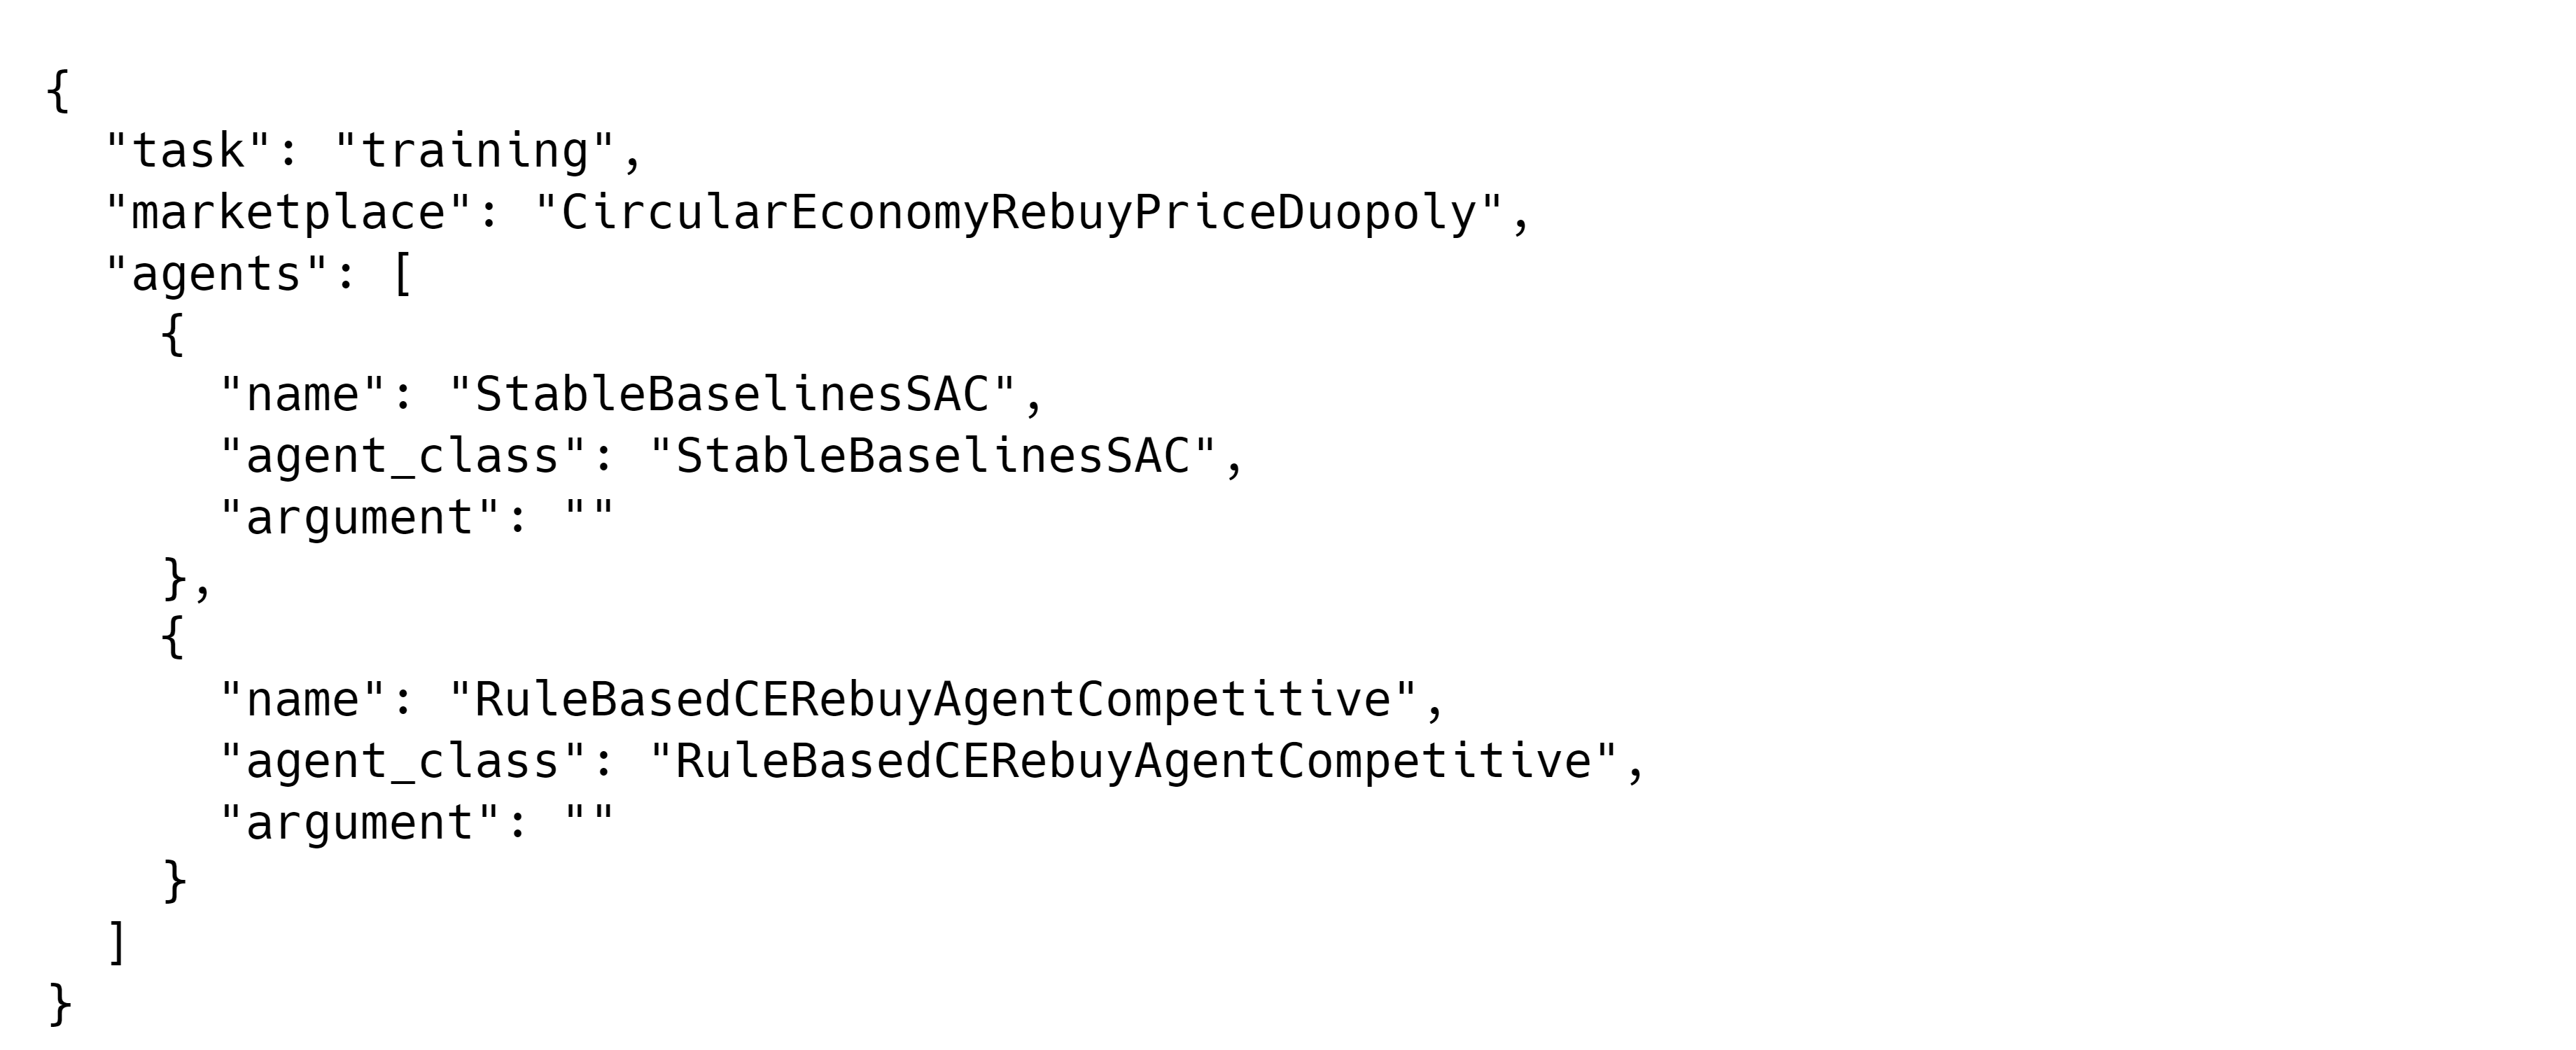
\includegraphics[width = 0.95\textwidth]{images/configs/SACDuopoly/SACDuopolyEnvironment.png}\\
	\caption{The \texttt{environment\_config.json} of the SAC-Duopoly experiment, simplified for readability.}\label{fig:SACDuopolyConfigEnvironment}
\end{figure}

\begin{figure}[ht]
	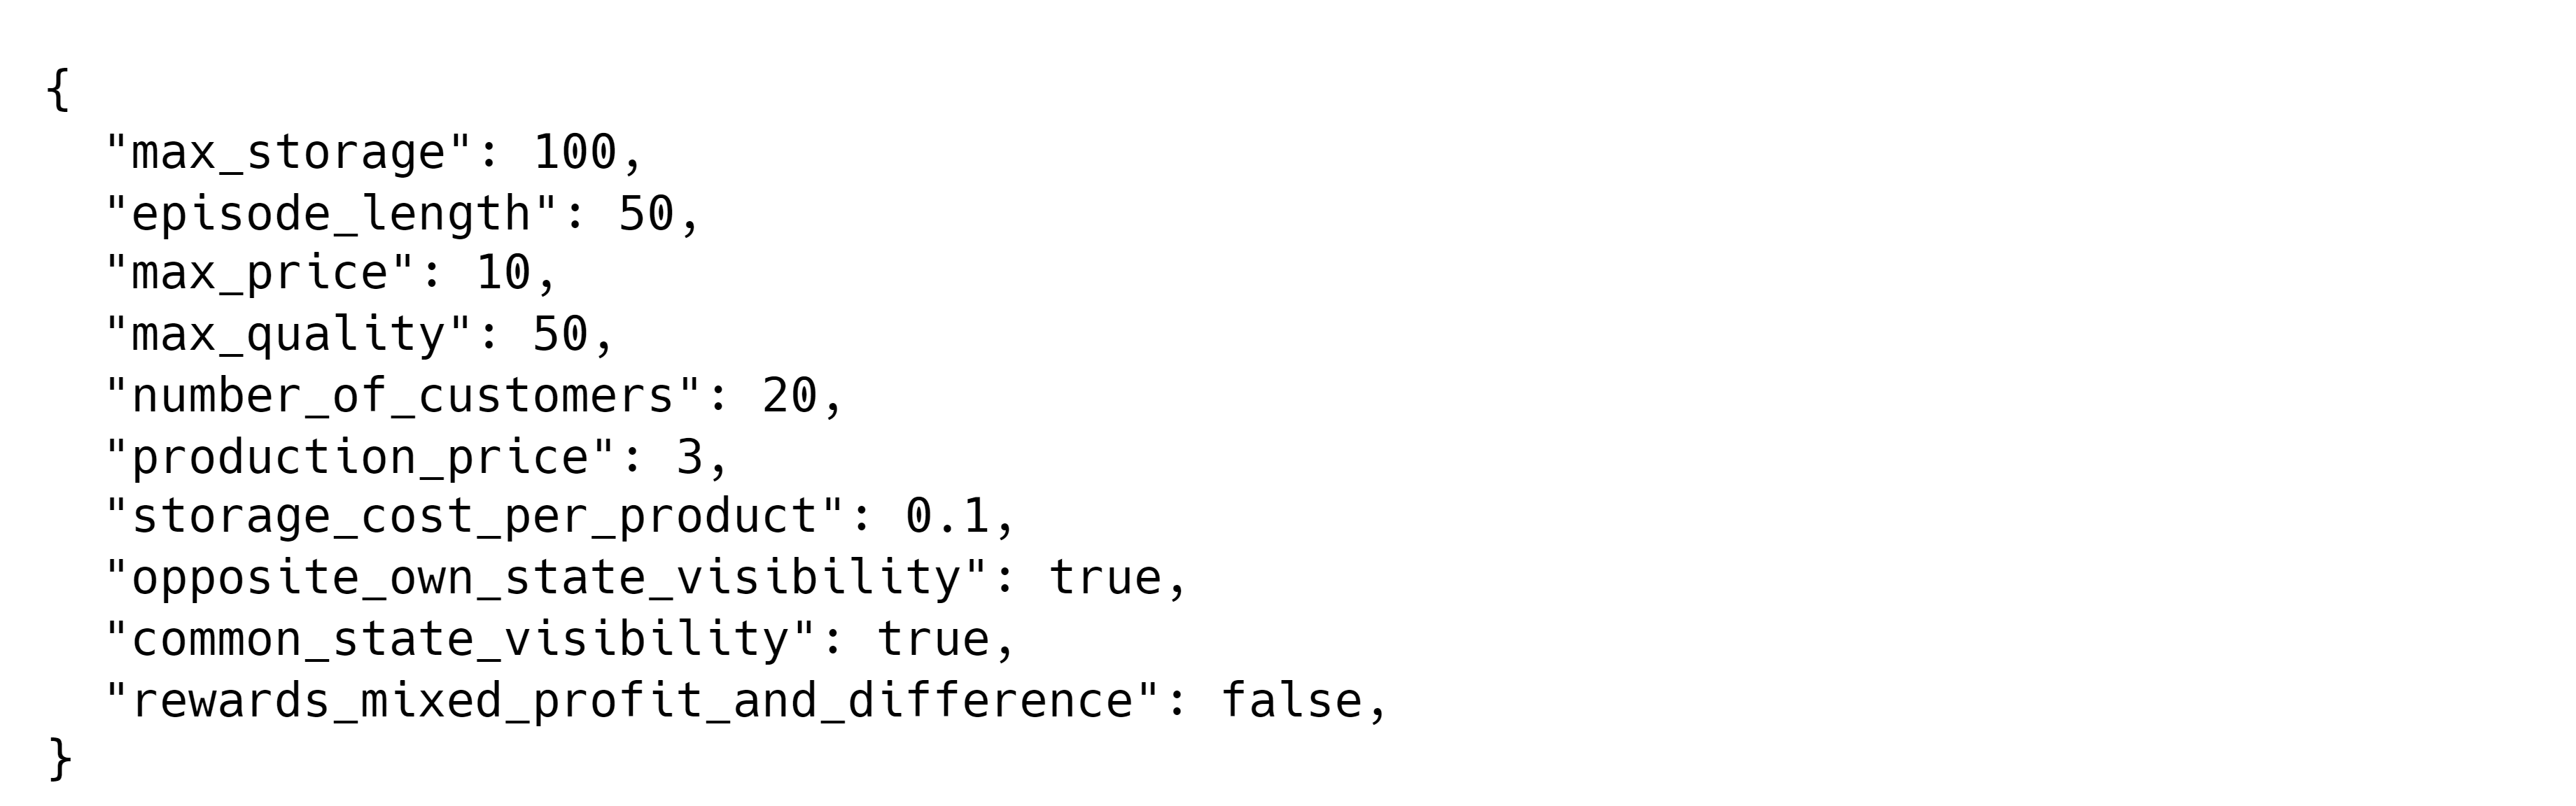
\includegraphics[width = 0.95\textwidth]{images/configs/SACDuopoly/SACDuopolyMarket.png}\\
	\caption{The \texttt{market\_config.json} of the SAC-Duopoly experiment.}\label{fig:SACDuopolyConfigMarket}
\end{figure}

\begin{figure}[ht]
	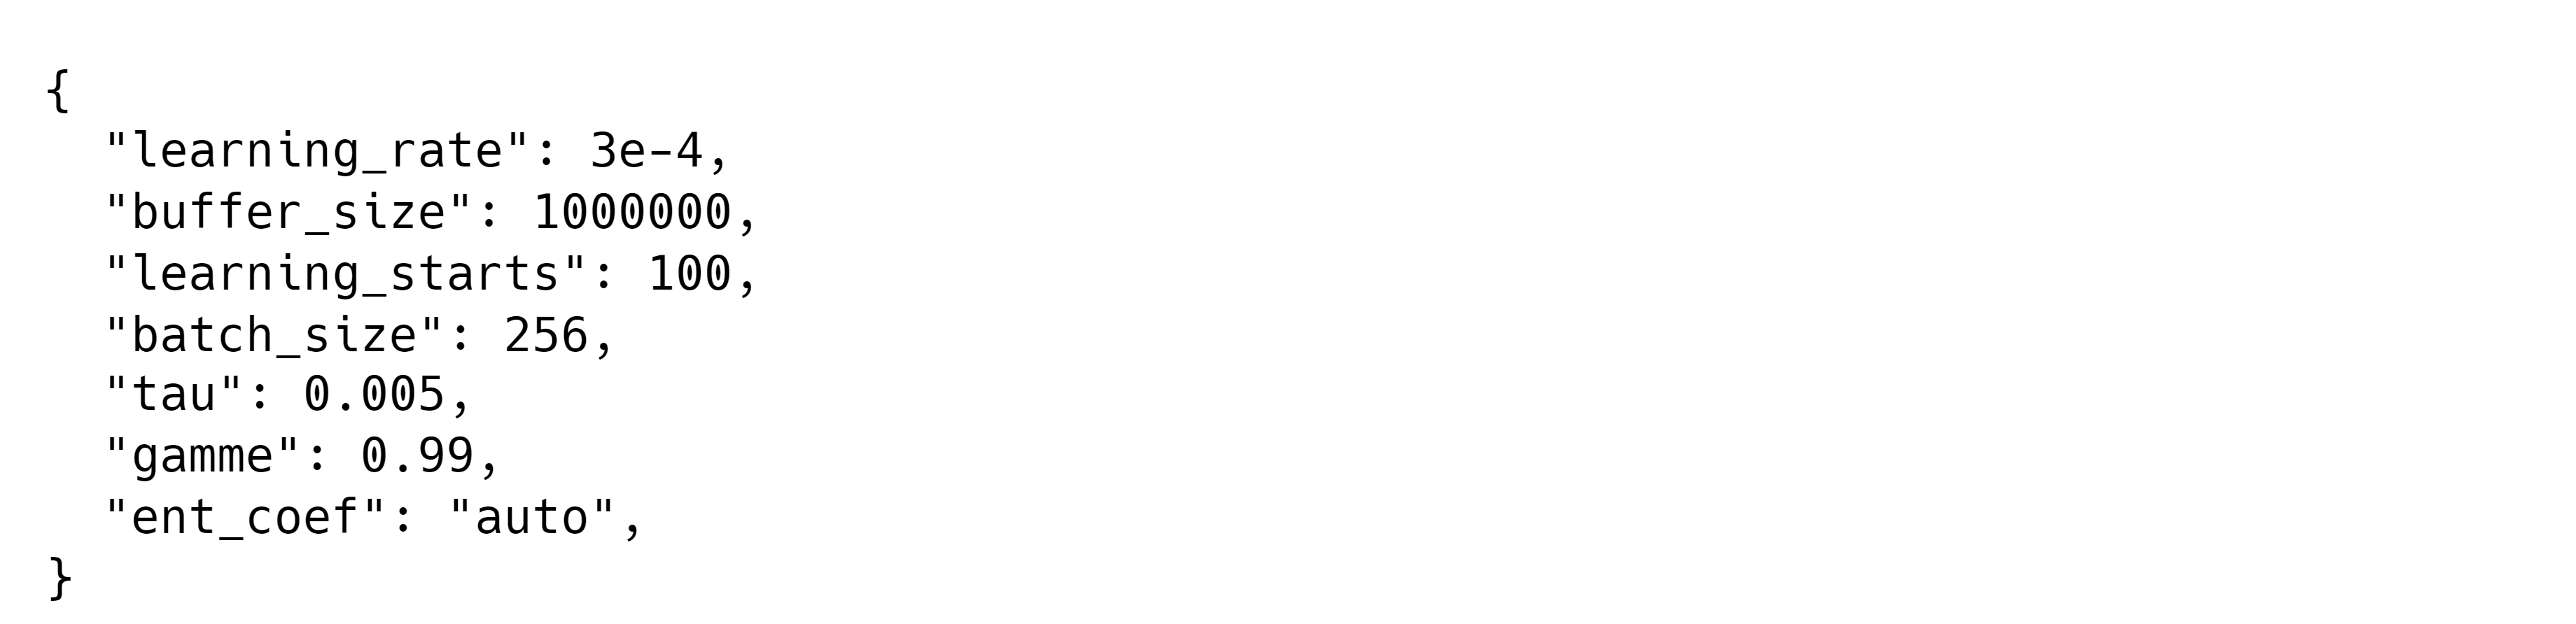
\includegraphics[width = 0.95\textwidth]{images/configs/SACDuopoly/SACDuopolyAgent.png}\\
	\caption{The configuration file for the SAC-Agent of the SAC-Duopoly experiment.}\label{fig:SACDuopolyConfigAgent}
\end{figure}

\clearpage
\section{PPO-Oligopoly experiment}\label{sec:AppendixOligopoly}

\subsection{Configuration files}\label{sec:AppendixOligopolyConfig}

The \texttt{market\_config.json} is the same as the one for the SAC-Duopoly experiment and can be found in \Cref{fig:SACDuopolyConfigMarket}.

\begin{figure}[ht]
	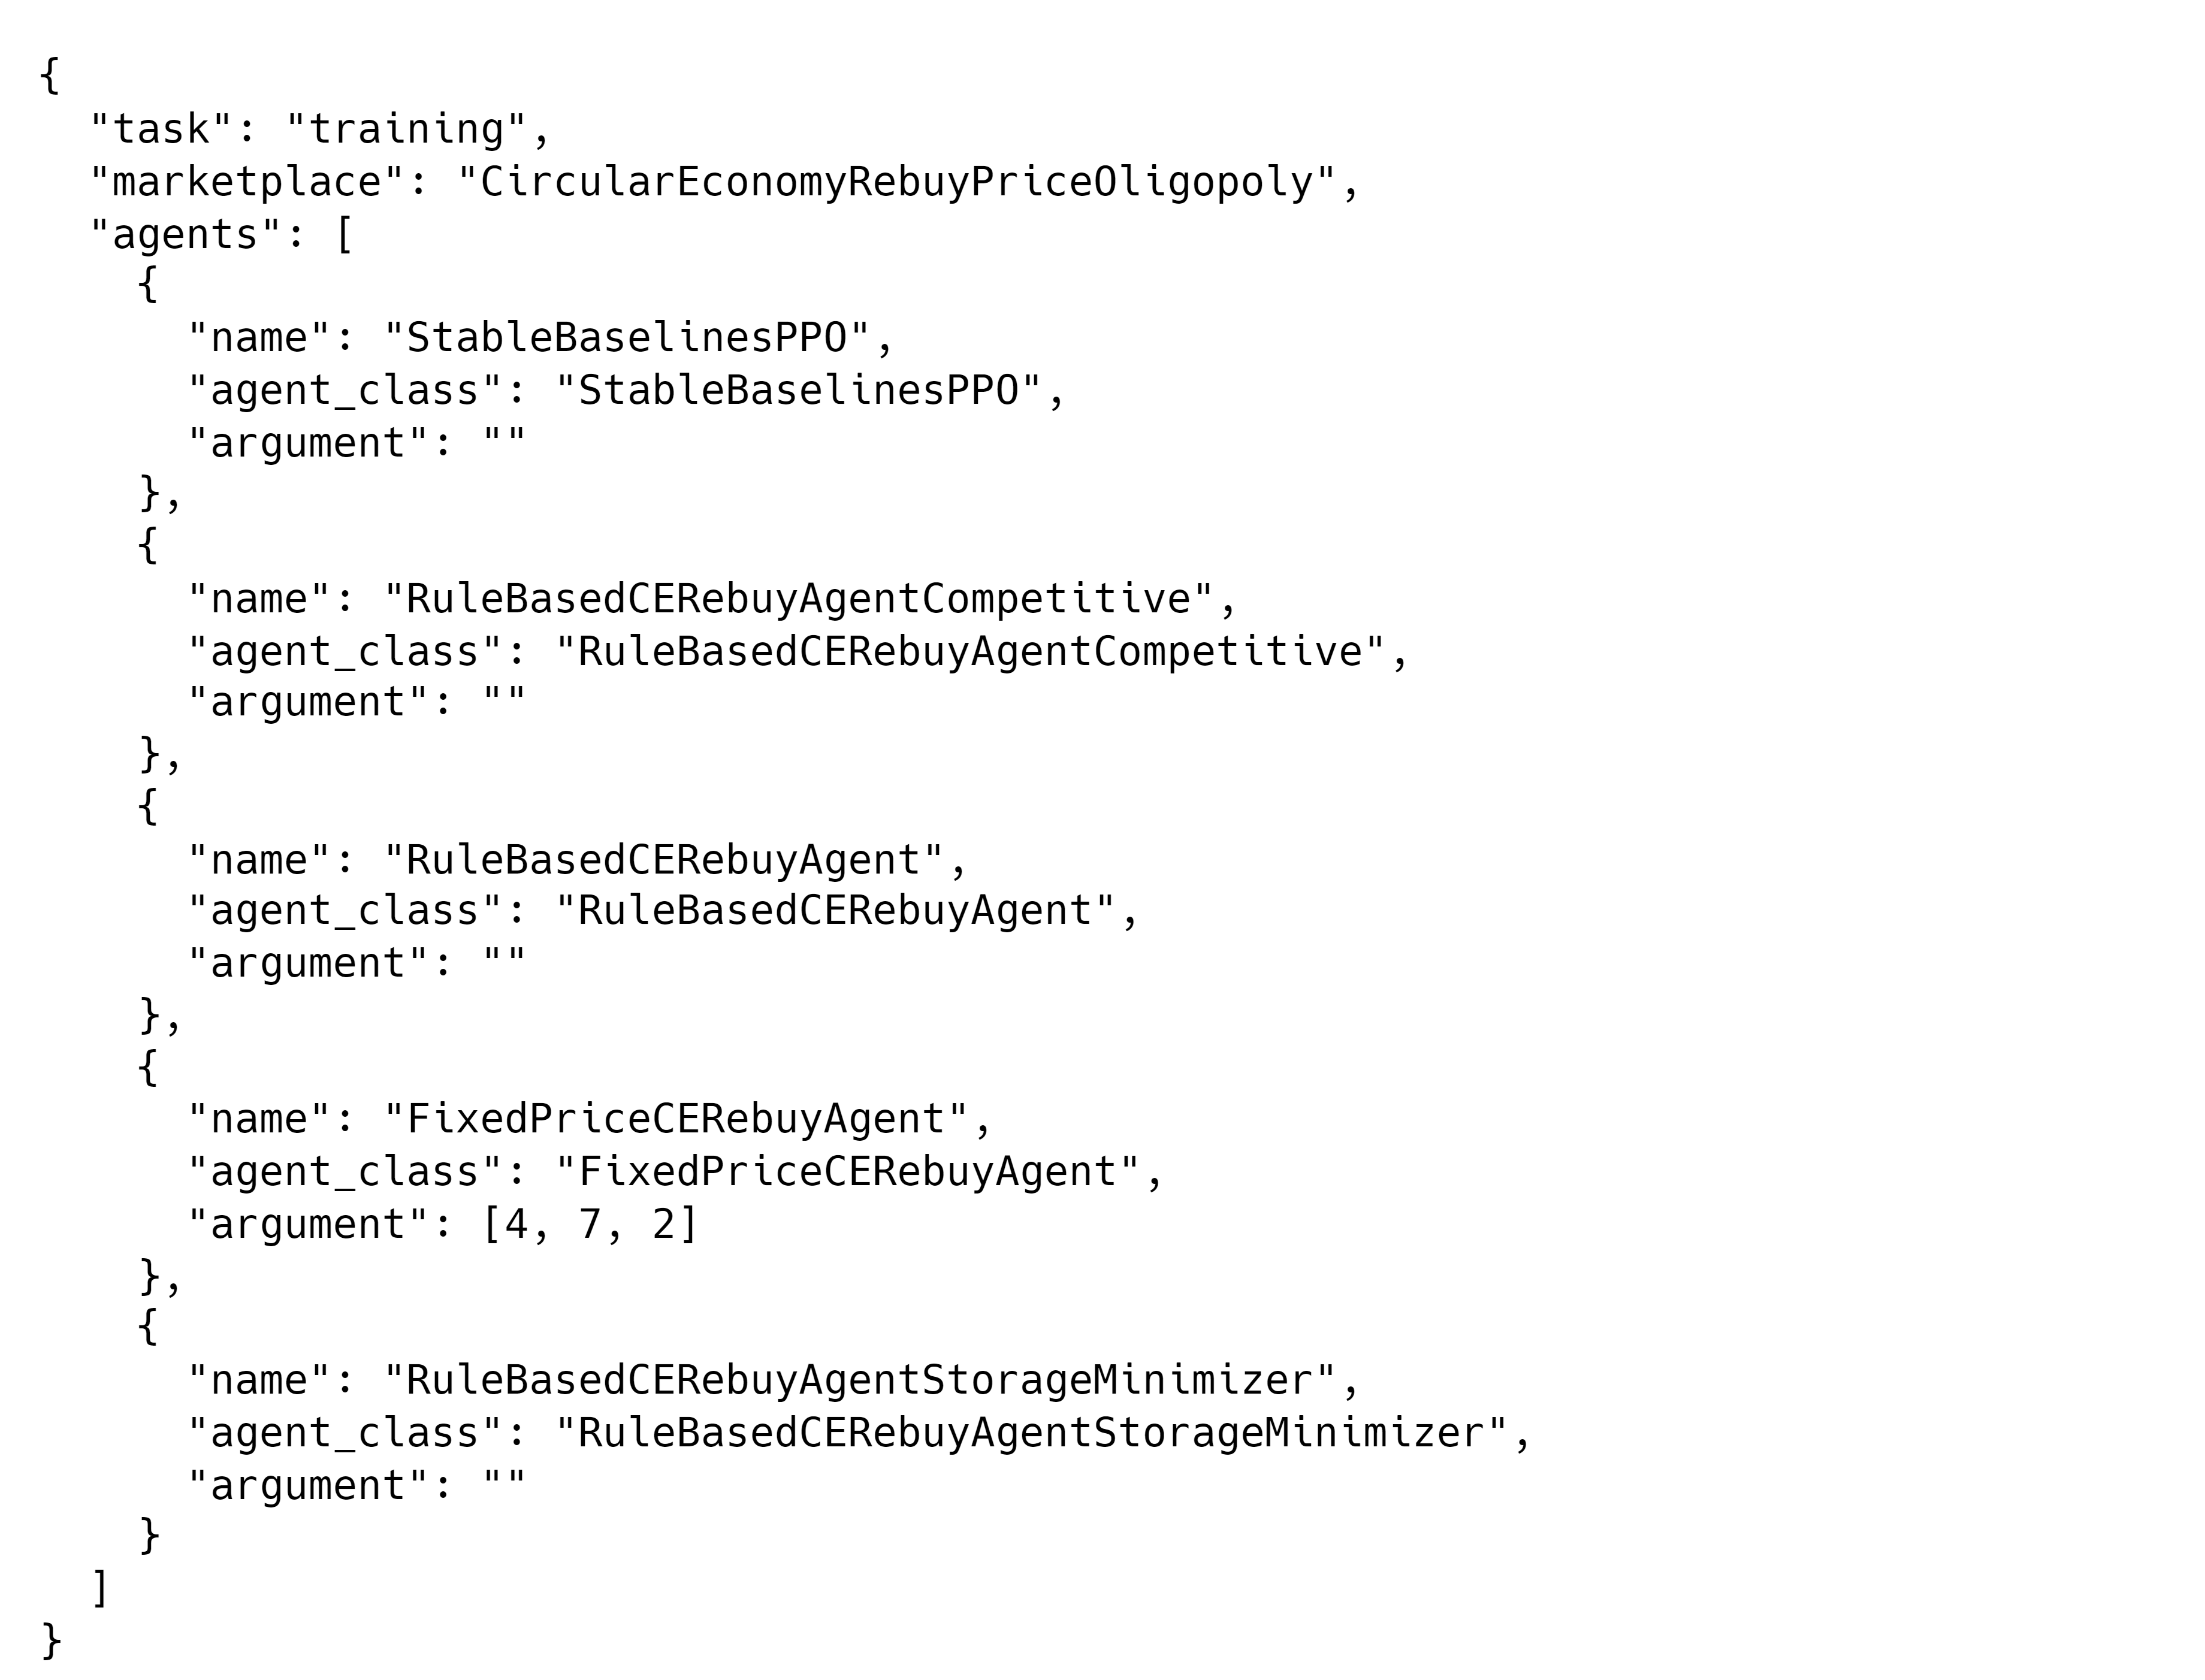
\includegraphics[width = \textwidth]{images/configs/PPOOligopoly/PPOOligopolyEnvironment.png}\\
	\caption{The \texttt{environment\_config.json} of the PPO-Oligopoly experiment, simplified for readability.}\label{fig:PPOOligopolyConfigEnvironment}
\end{figure}

\begin{figure}[ht]
	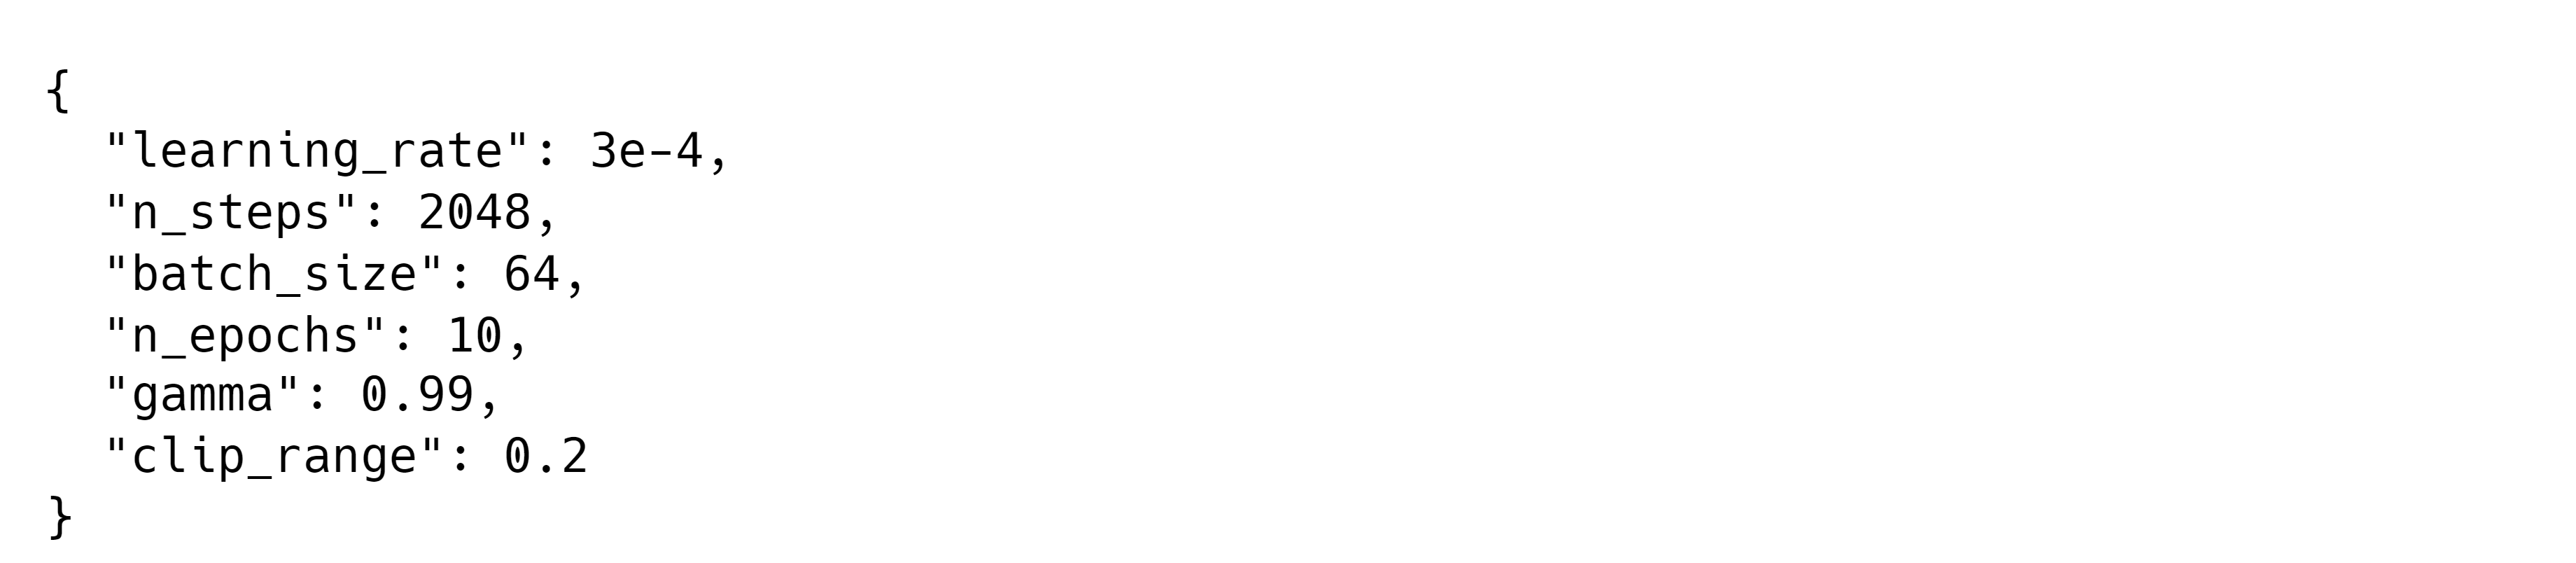
\includegraphics[width = \textwidth]{images/configs/PPOOligopoly/PPOOligopolyAgent.png}\\
	\caption{The configuration file for the PPO-Agent of the PPO-Oligopoly experiment.}\label{fig:PPOOligopolyConfigAgent}
\end{figure}

\clearpage
\subsection{Diagrams}\label{sec:AppendixOligopolyDiagrams}

Some of the more interesting diagrams created during the training and subsequent Live-monitoring of the PPO-Oligopoly experiment are shown here, without in-depth interpretation. The agent was trained for a total of 5,000 episodes. Following the standard Oligopoly setup, all vendors played at the same time, setting prices after one another within each step.

% All profits + cum profits histogram
\begin{figure}[ht]
	\centering
	\begin{subfigure}[t]{0.49\textwidth}
		\centering
		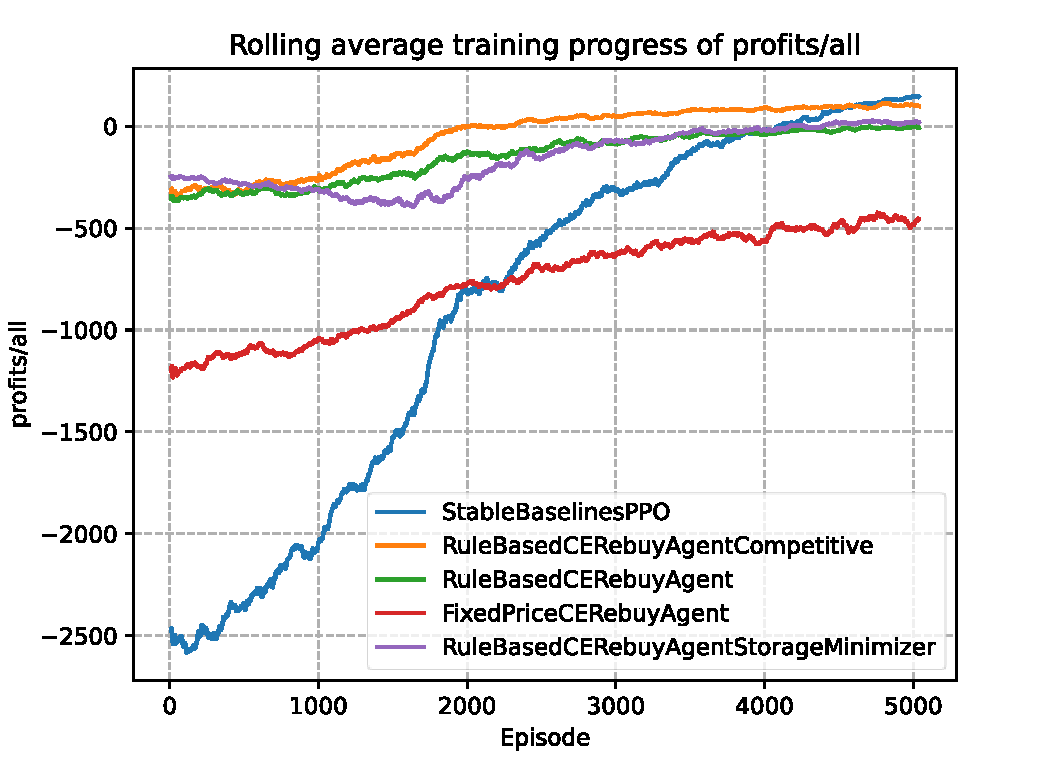
\includegraphics[width = \textwidth]{images/experiments/PPOOligopoly/PPOOligopolyLineProfitsAll.pdf}\\
		\subcaption{Profits per episode achieved during the training run}\label{fig:PPOOligopolyLineProfitsAll}
	\end{subfigure}
	\begin{subfigure}[t]{0.49\textwidth}
		\centering
		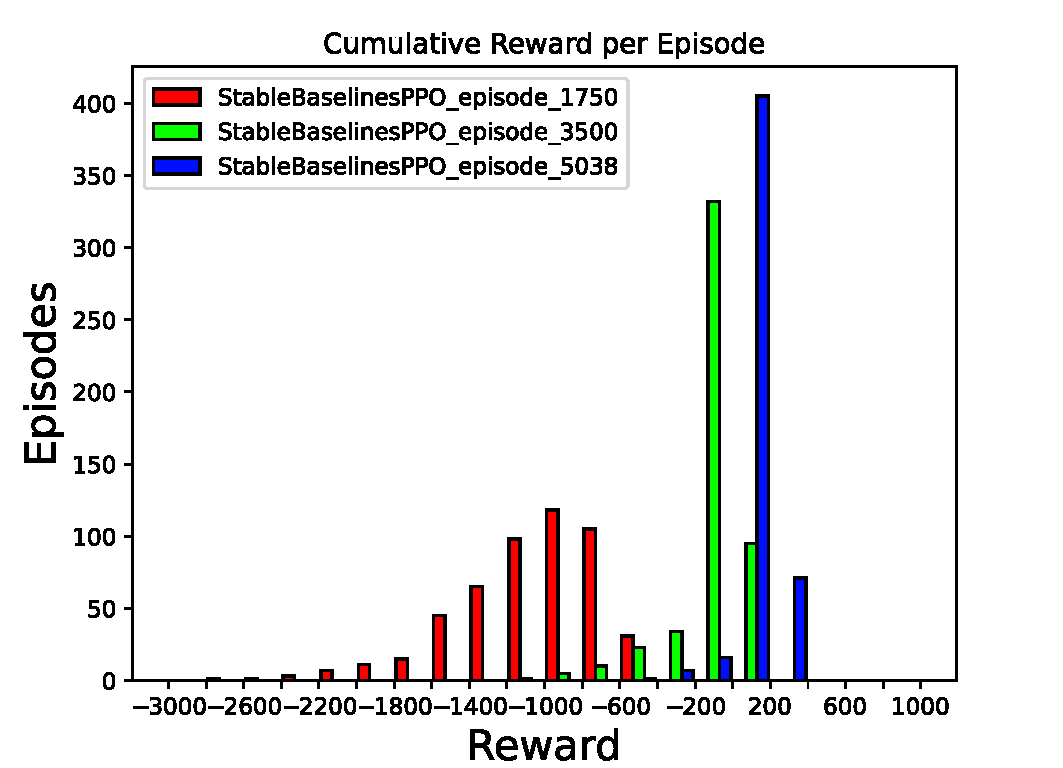
\includegraphics[width = \textwidth]{images/experiments/PPOOligopoly/PPOOligopolyCumulativeRewards.pdf}\\
		\subcaption{Cumulative rewards per training stage per interval, recorded during the Agent-monitoring session}\label{fig:PPOOligopolyCumulativeRewards}
	\end{subfigure}
	\caption{The PPO-Agent took significantly longer than the SAC-Agent (\Cref{fig:SACDuopolyProfitsMean}) to reach its maximum possible profit (\Cref{fig:PPOOligopolyLineProfitsAll}) and the model that was trained longest outperforms the other two (\Cref{fig:PPOOligopolyCumulativeRewards}), as was to be expected following the steady increase in profits during training.}\label{fig:PPOOligopolyMixed}
\end{figure}

% price rebuy + price refurb
\begin{figure}[ht]
	\centering
	\begin{subfigure}[t]{0.49\textwidth}
		\centering
		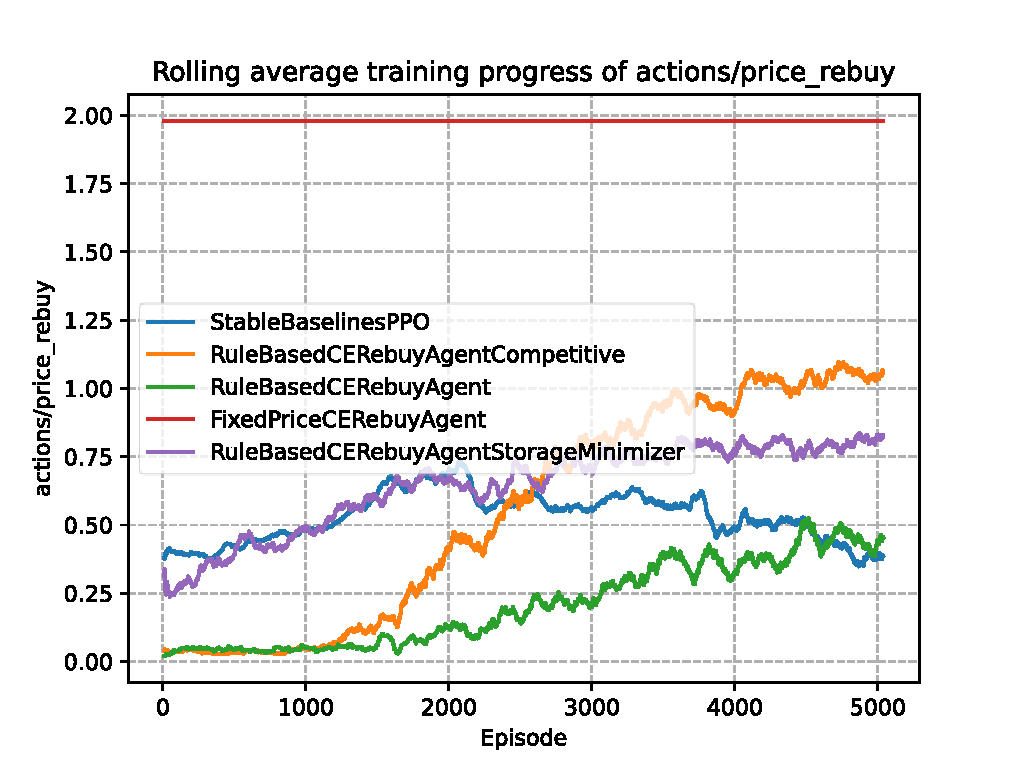
\includegraphics[width = \textwidth]{images/experiments/PPOOligopoly/PPOOligopolyLinePriceRebuy.pdf}\\
		\subcaption{Rebuy prices}\label{fig:PPOOligopolyLinePriceRebuy}
	\end{subfigure}
	\begin{subfigure}[t]{0.49\textwidth}
		\centering
		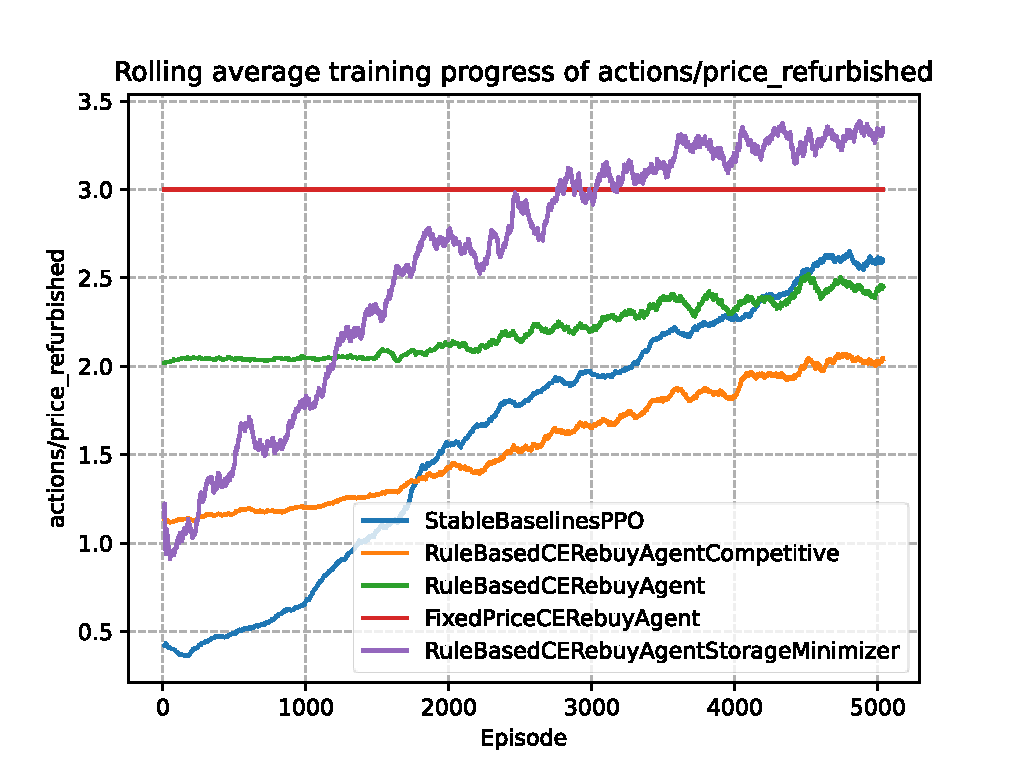
\includegraphics[width = \textwidth]{images/experiments/PPOOligopoly/PPOOligopolyLinePriceRefurbished.pdf}\\
		\subcaption{Prices for refurbished products}\label{fig:PPOOligopolyLinePriceRefurbished}
	\end{subfigure}
	\caption{While rebuy prices were consistently at or below 1 (excluding the \emph{FixedPriceAgent}), prices for refurbished products rose consistently, with the \emph{RuleBasedCERebuyAgentStorageMinimizer} leading the price run.}\label{fig:PPOOligopolyDiagramsPrices}
\end{figure}


% purch refurb + storage costs
\begin{figure}[ht]
	\centering
	\begin{subfigure}[t]{0.49\textwidth}
		\centering
		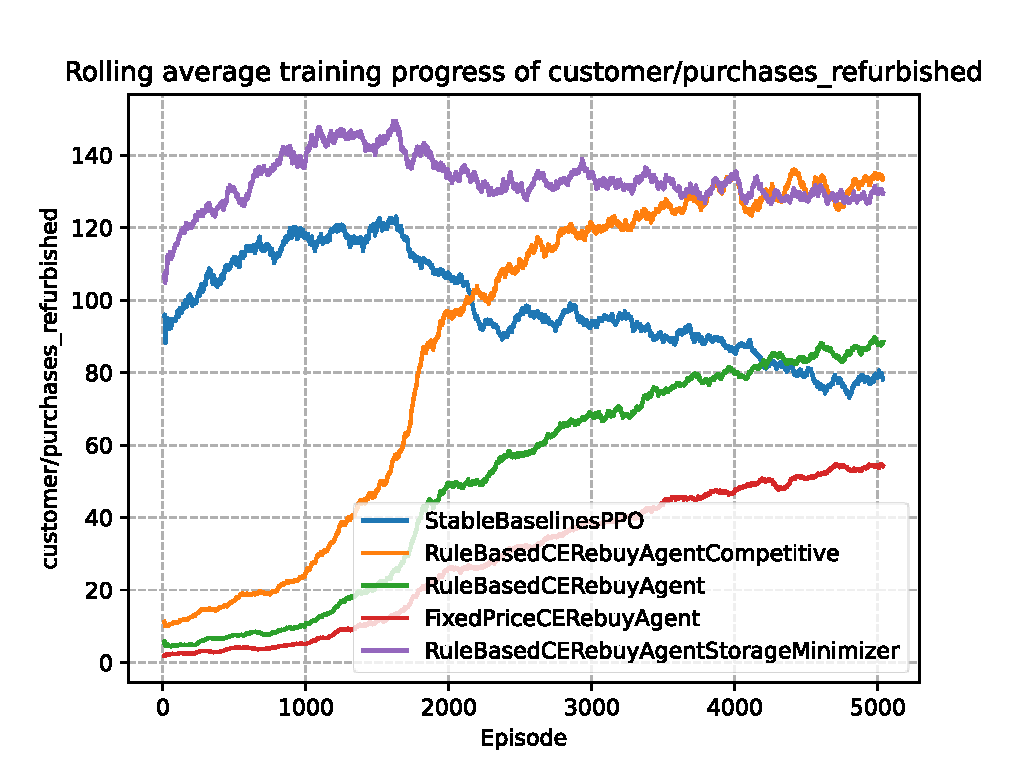
\includegraphics[width = \textwidth]{images/experiments/PPOOligopoly/PPOOligopolyLinePurchasesRefurbished.pdf}\\
		\subcaption{Number of purchases of refurbished products}\label{fig:PPOOligopolyLinePurchasesRefurbished}
	\end{subfigure}
	\begin{subfigure}[t]{0.49\textwidth}
		\centering
		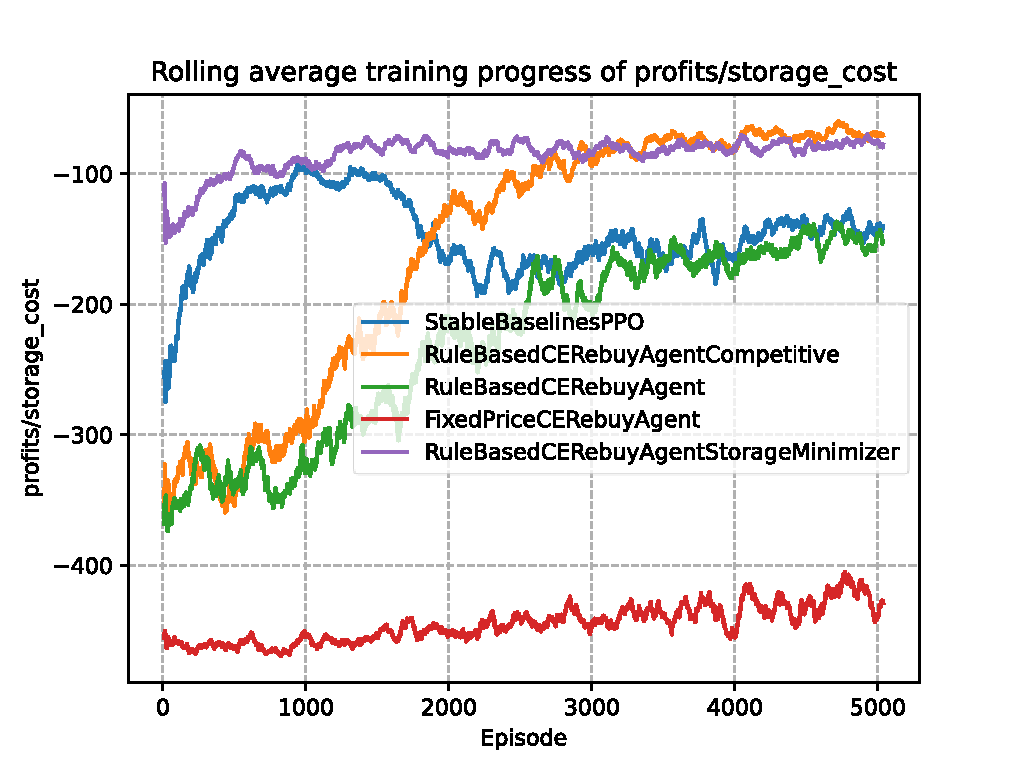
\includegraphics[width = \textwidth]{images/experiments/PPOOligopoly/PPOOligopolyLineStorageCosts.pdf}\\
		\subcaption{Storage costs per episode}\label{fig:PPOOligopolyLineStorageCosts}
	\end{subfigure}
	\caption{Except in the case of the \emph{FixedPriceAgent}, a higher number of sales of refurbished products was always followed by a similar decrease in storage costs, meaning that the number of bought back products likely stayed on a steady level over the course of training. This is confirmed by \Cref{fig:PPOOligopolyLineOwnerRebuys}.}\label{fig:PPOOligopolyDiagramsPurchases}
\end{figure}

% rebuys + buy nothing
\begin{figure}[ht]
	\centering
	\begin{subfigure}[t]{0.49\textwidth}
		\centering
		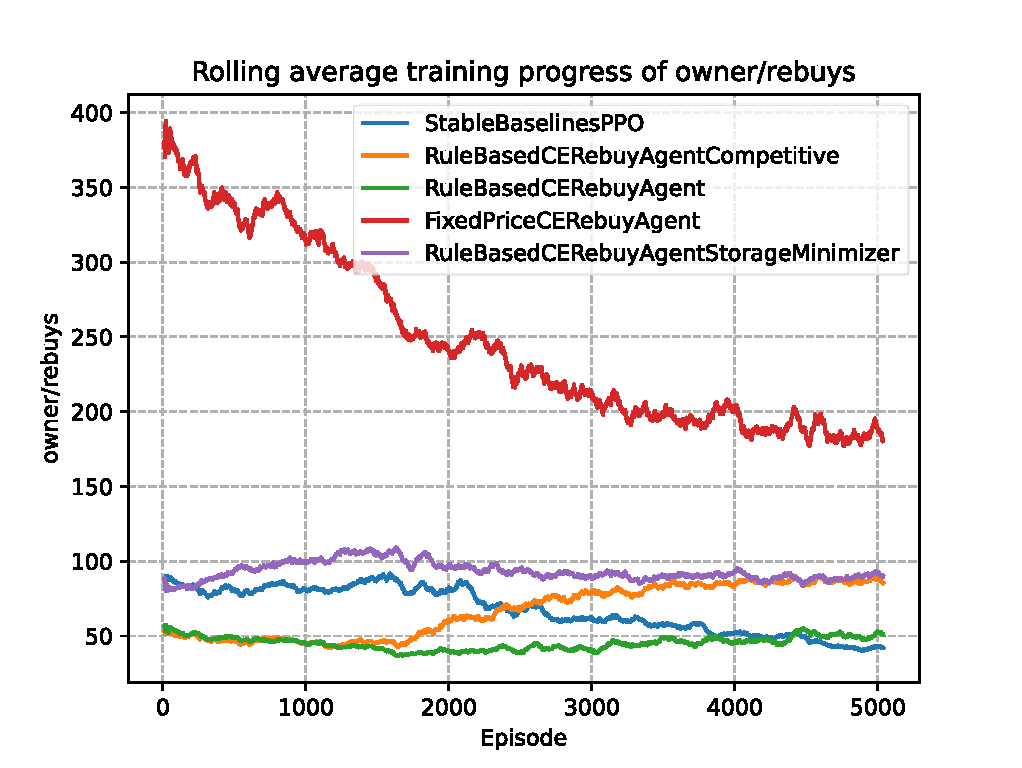
\includegraphics[width = \textwidth]{images/experiments/PPOOligopoly/PPOOligopolyLineOwnerRebuys.pdf}\\
		\subcaption{Number of products bought back by each vendor}\label{fig:PPOOligopolyLineOwnerRebuys}
	\end{subfigure}
	\begin{subfigure}[t]{0.49\textwidth}
		\centering
		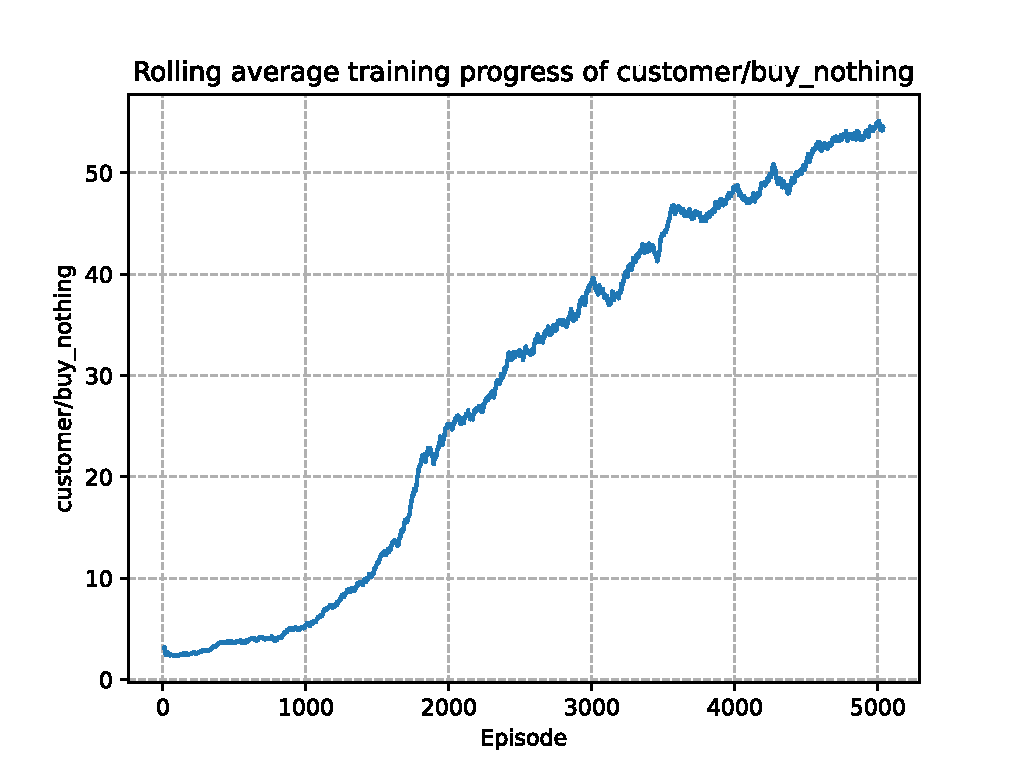
\includegraphics[width = \textwidth]{images/experiments/PPOOligopoly/PPOOligopolyLineBuyNothing.pdf}\\
		\subcaption{Number of customers that bought no product}\label{fig:PPOOligopolyLineBuyNothing}
	\end{subfigure}
	\caption{The number of products bought back by vendors (except for the \emph{FixedPriceAgent}) stayed similar over the whole course of training. With an increase in rebuy-prices (\Cref{fig:PPOOligopolyLinePriceRebuy}), the \emph{FixedPriceAgent} lost some of its rebuys to the other vendors. Following an overall increase in prices (see e.g. \Cref{fig:PPOOligopolyLinePriceRefurbished}), more and more customers chose to buy none of the advertised products.}\label{fig:PPOOligopolyDiagramsOwners}
\end{figure}

\addchap{Declaration of Authorship}
I hereby declare that this thesis is my own unaided work. All direct or indirect sources used are acknowledged as references.\\[6 ex]

\begin{flushleft}
    Potsdam, \today
    \hspace*{2 em}
    \raisebox{-0.9\baselineskip}
    {
        \begin{tabular}{p{5 cm}}
            \hline
            \centering\footnotesize\printAuthor
        \end{tabular}
    }
\end{flushleft}


\end{document}